\chapter{Results \& Discussion} \label{chap:results}
In this chapter I present the results of the $\chi^2$ test and the SBI. In addition, I discuss these results and explain the observed patterns. I plot the data points of DM-$z$ from the true and contaminated catalogs in the DM-$z$ plane and show the mean in a line and the corresponding 1$\sigma$ as a shaded area, as will be shown in the following sections.

In general, the systematic scenarios considered in this thesis are simple, therefore, they provide a lower limit on the bias caused by each of these uncertainties.


\section{Results from the Chi-Squared Test}
In this section, I present the results of the $\chi^2$ test for all the 5 systematic uncertainties that I am tackling in this thesis.

\subsection{Milky Way Contribution}
The MW uncertainty is added by taking a true mock catalog and adding the corresponding MW contribution as predicted by the NPE2001 model. As can be seen from Fig. \ref{theory_fig:MW_map}, the largest $\mathrm{DM}_\mathrm{MW}$ corresponds to sources that are located near the galactic plane. Therefore, Figs. \ref{res_fig:mw_dmz_pdf} shows the variation of the PDF and the DM-$z$ relation with changing galactic cut. In general, $\mathrm{DM}_\mathrm{MW}$ adds a component to $\mathrm{DM}_\mathrm{tot}$ which ultimately modifies the mean DM and adds a component to the variance. This can be seen from the left-hand side of Fig. \ref{res_fig:mw_dmz_pdf}. By looking at the right-hand side of Fig. \ref{res_fig:mw_dmz_pdf}, the PDF changes when adding the $\mathrm{DM}_\mathrm{tot}$ with overall shift to the right. This corresponds to a changing mean for the overall PDF. Meanwhile, there is no obvious pattern for changing the variance.
\begin{figure}[h!]
    \centering
    \begin{subfigure}[t]{0.48\textwidth}
        \centering
        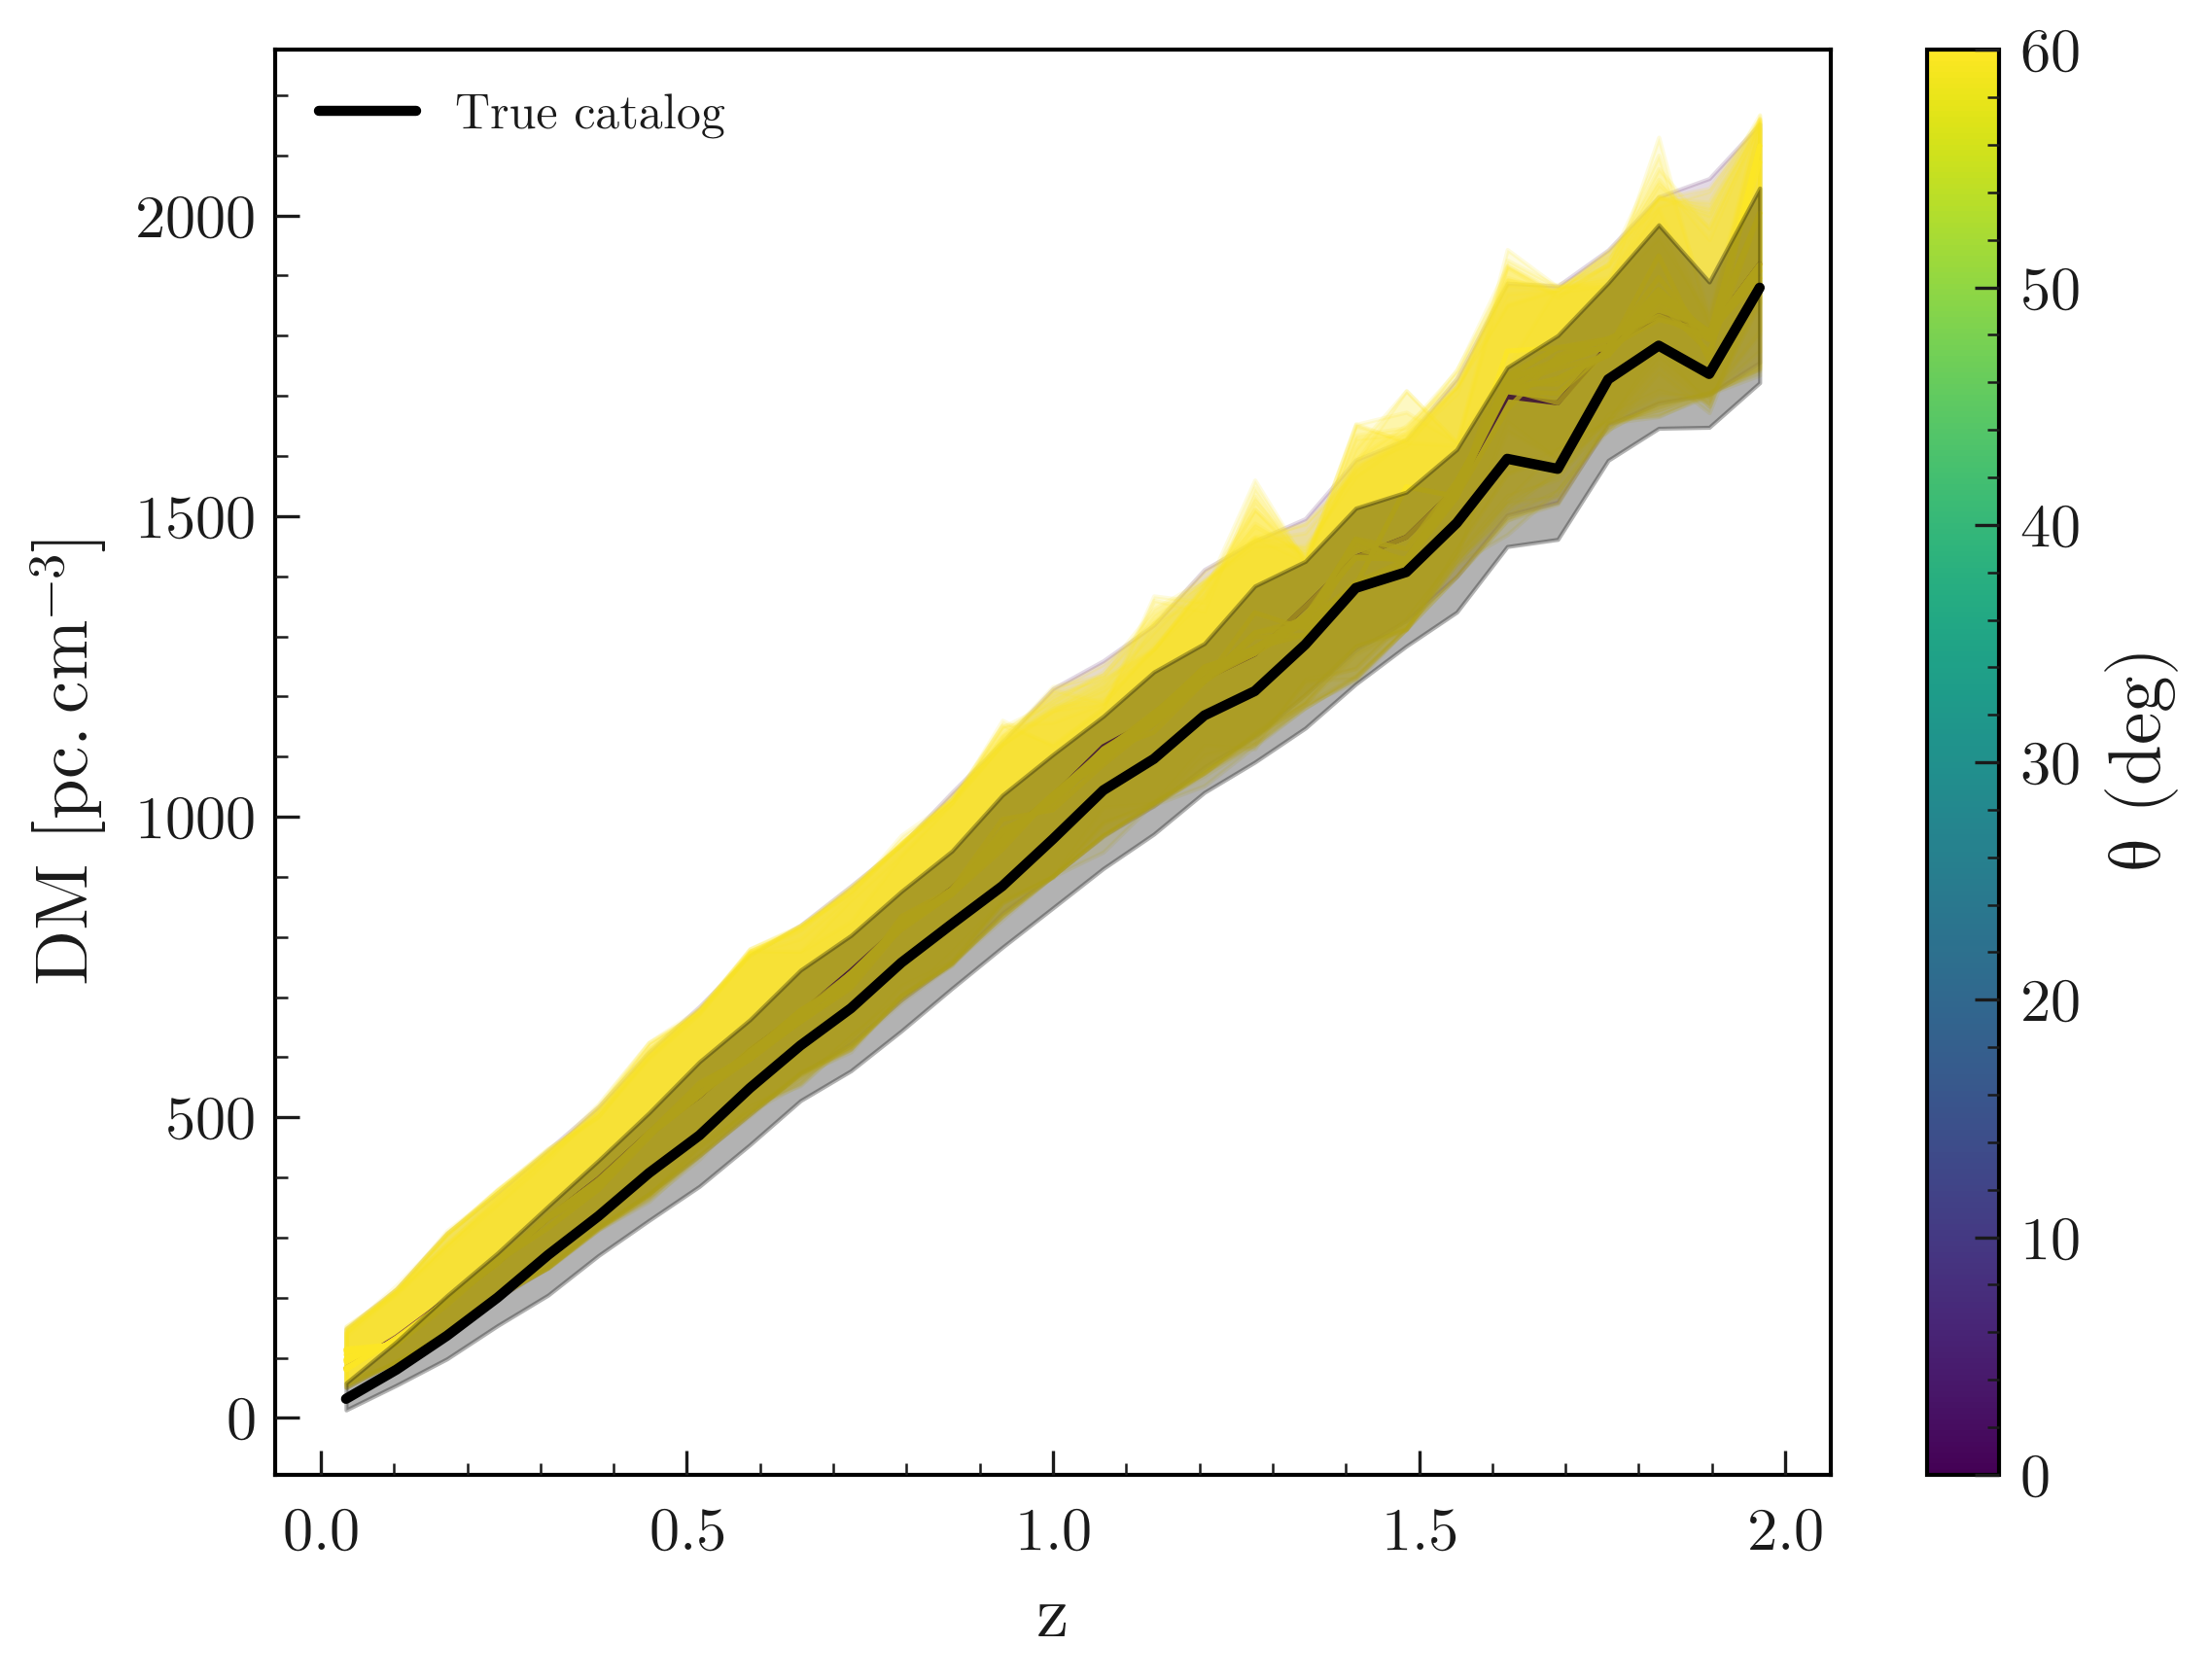
\includegraphics[width=\textwidth]{figs/dm_z_uncertainty_MW_contribution.png}
        \caption{DM-$z$ relation for varying Milky Way contribution.}
    \end{subfigure}
    \hfill
    \begin{subfigure}[t]{0.48\textwidth}
        \centering
        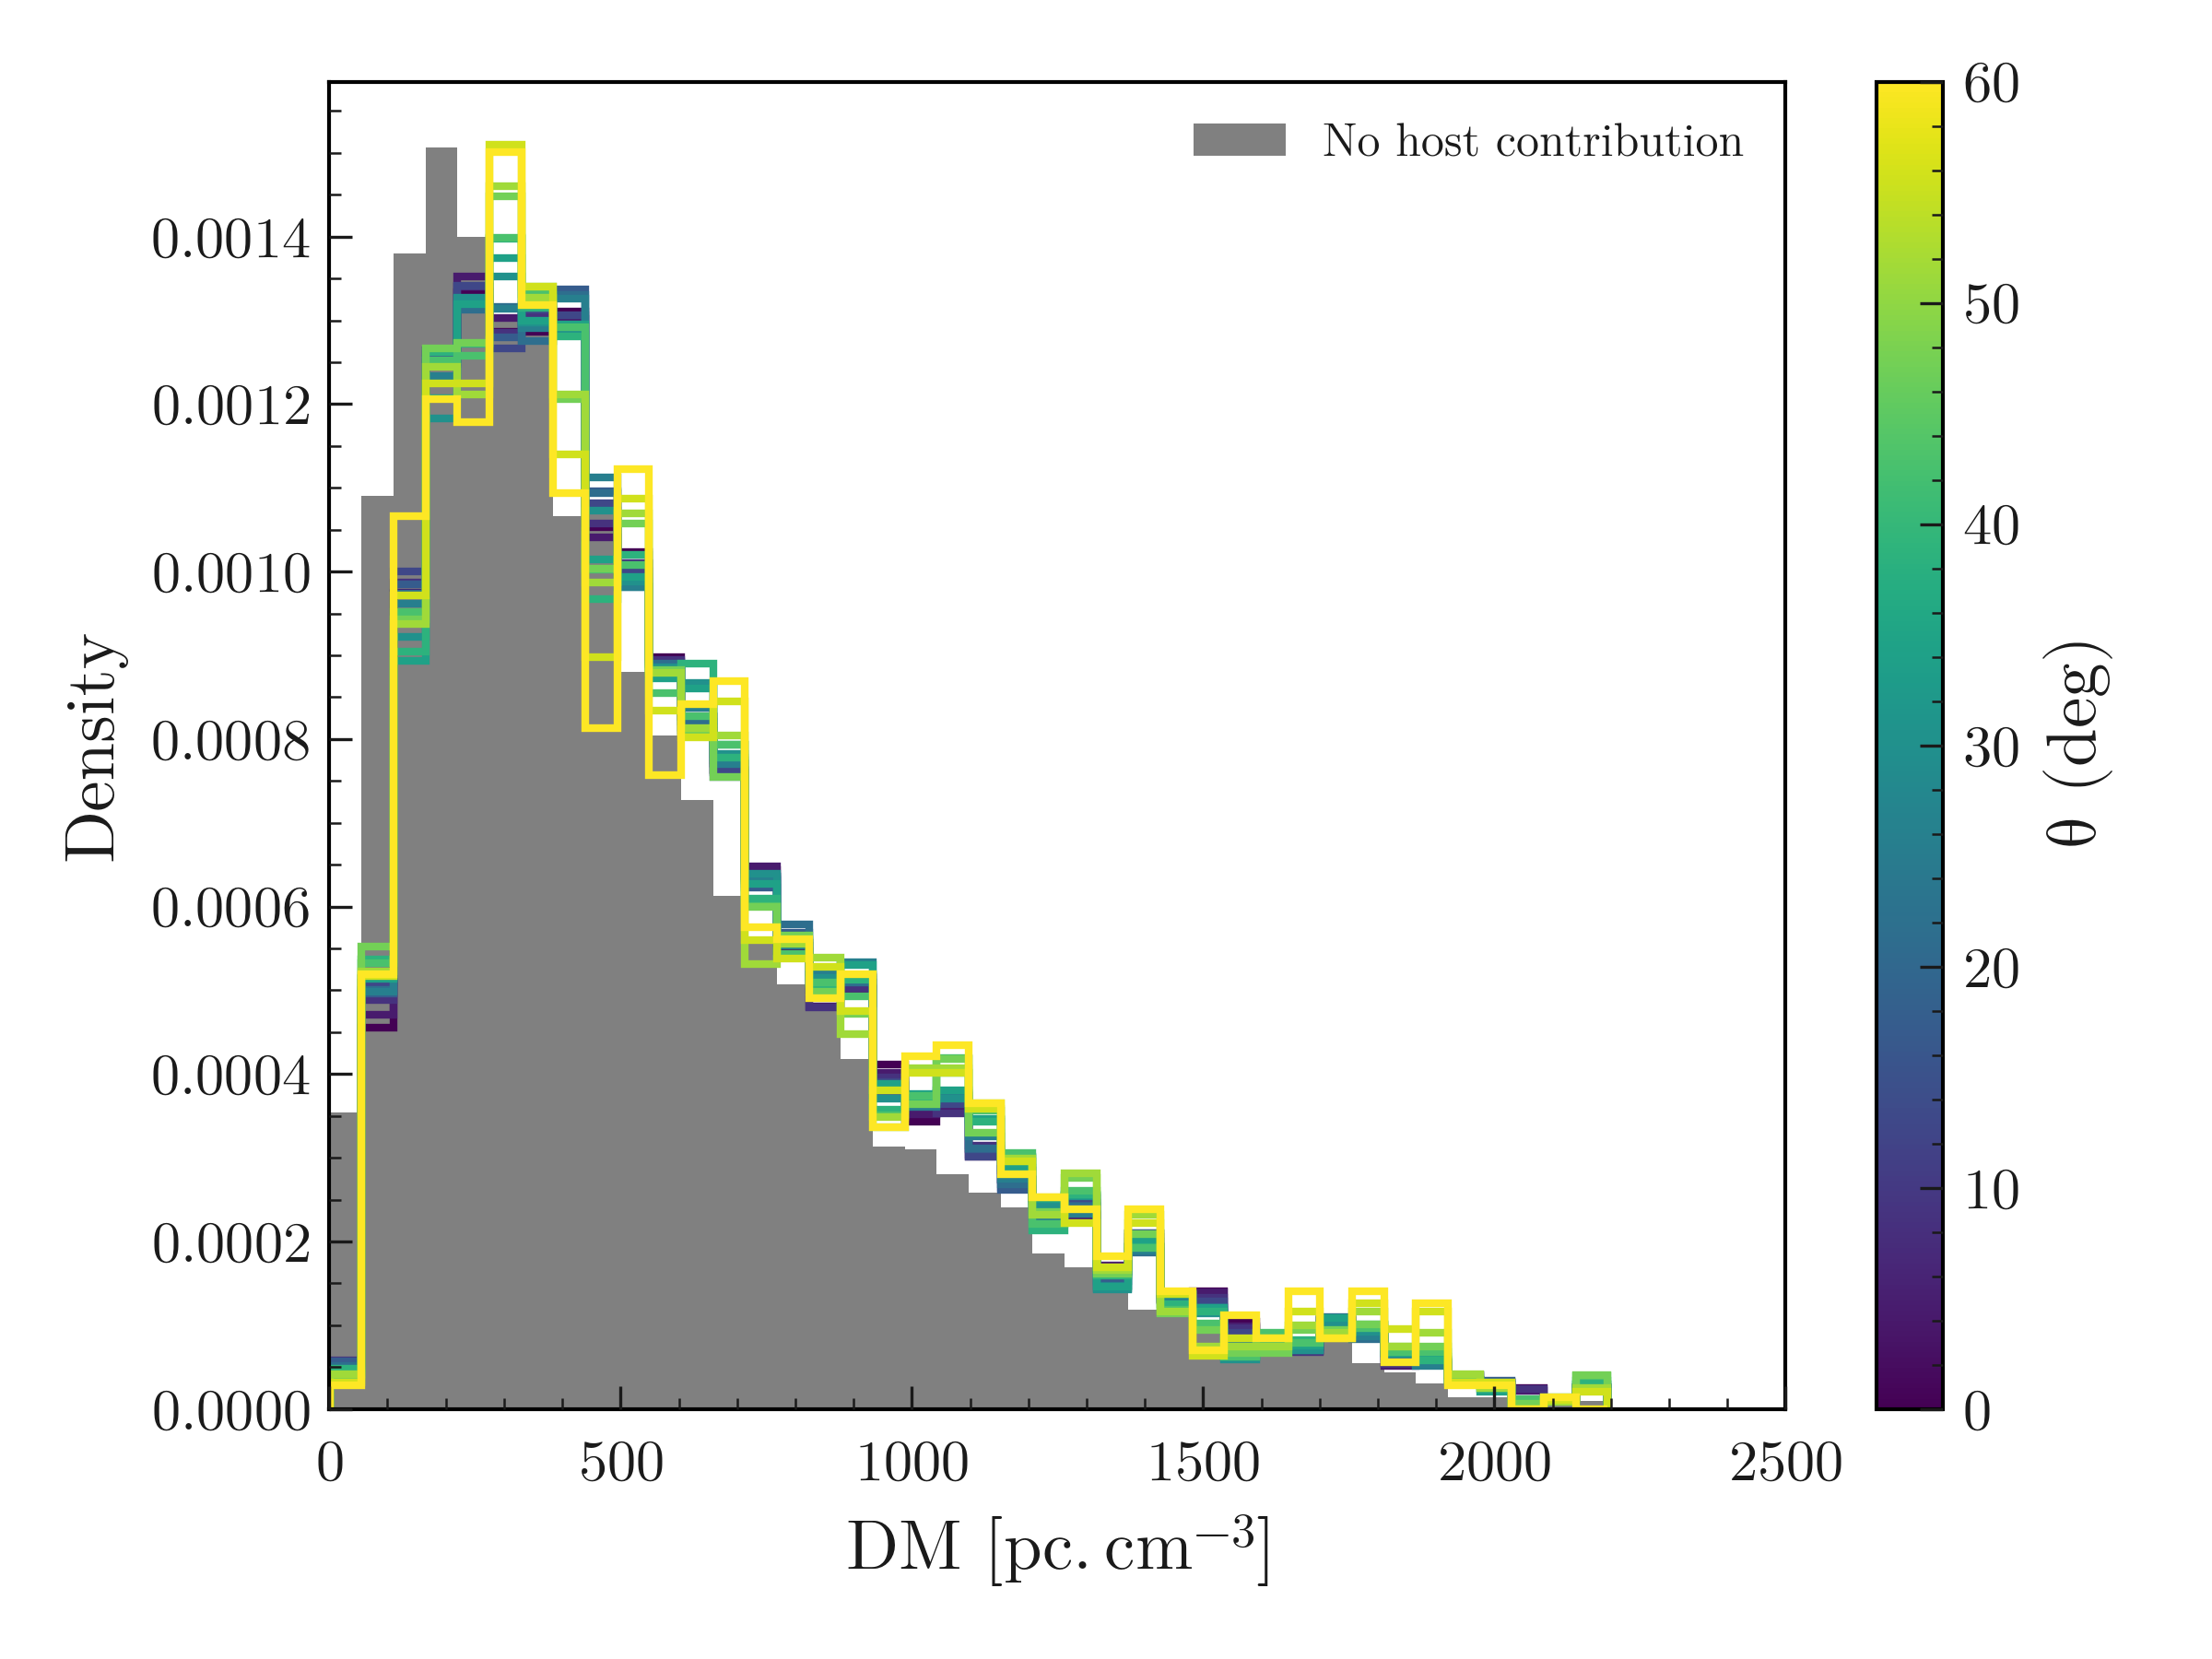
\includegraphics[width=\textwidth]{figs/pdf_uncertainty_MW_contribution.png}
        \caption{PDF of DM for varying Milky Way contribution.}
    \end{subfigure}
    \caption{DM-$z$ relation and PDF for the Milky Way contribution systematic.}
    \label{res_fig:mw_dmz_pdf}
\end{figure}
The variation of $\chi^2$ with galactic cut are shown in Fig. \ref{res_fig:mw_chisq}. For galactic cuts below 30 deg, the $\chi^2$ is larger than the true value, and it gets close to the true value around 30 deg and then decreases for larger galactic cuts. Therefore, it is possible to choose an appropriate galactic cut in order to mitigate the impact of MW contribution on the DM-$z$ relation. This result requires further verification by studying the variance and the mean of sky area that could be masked out due to having large $\mathrm{DM}_\mathrm{MW}$.




\begin{figure}[h!]
    \centering
    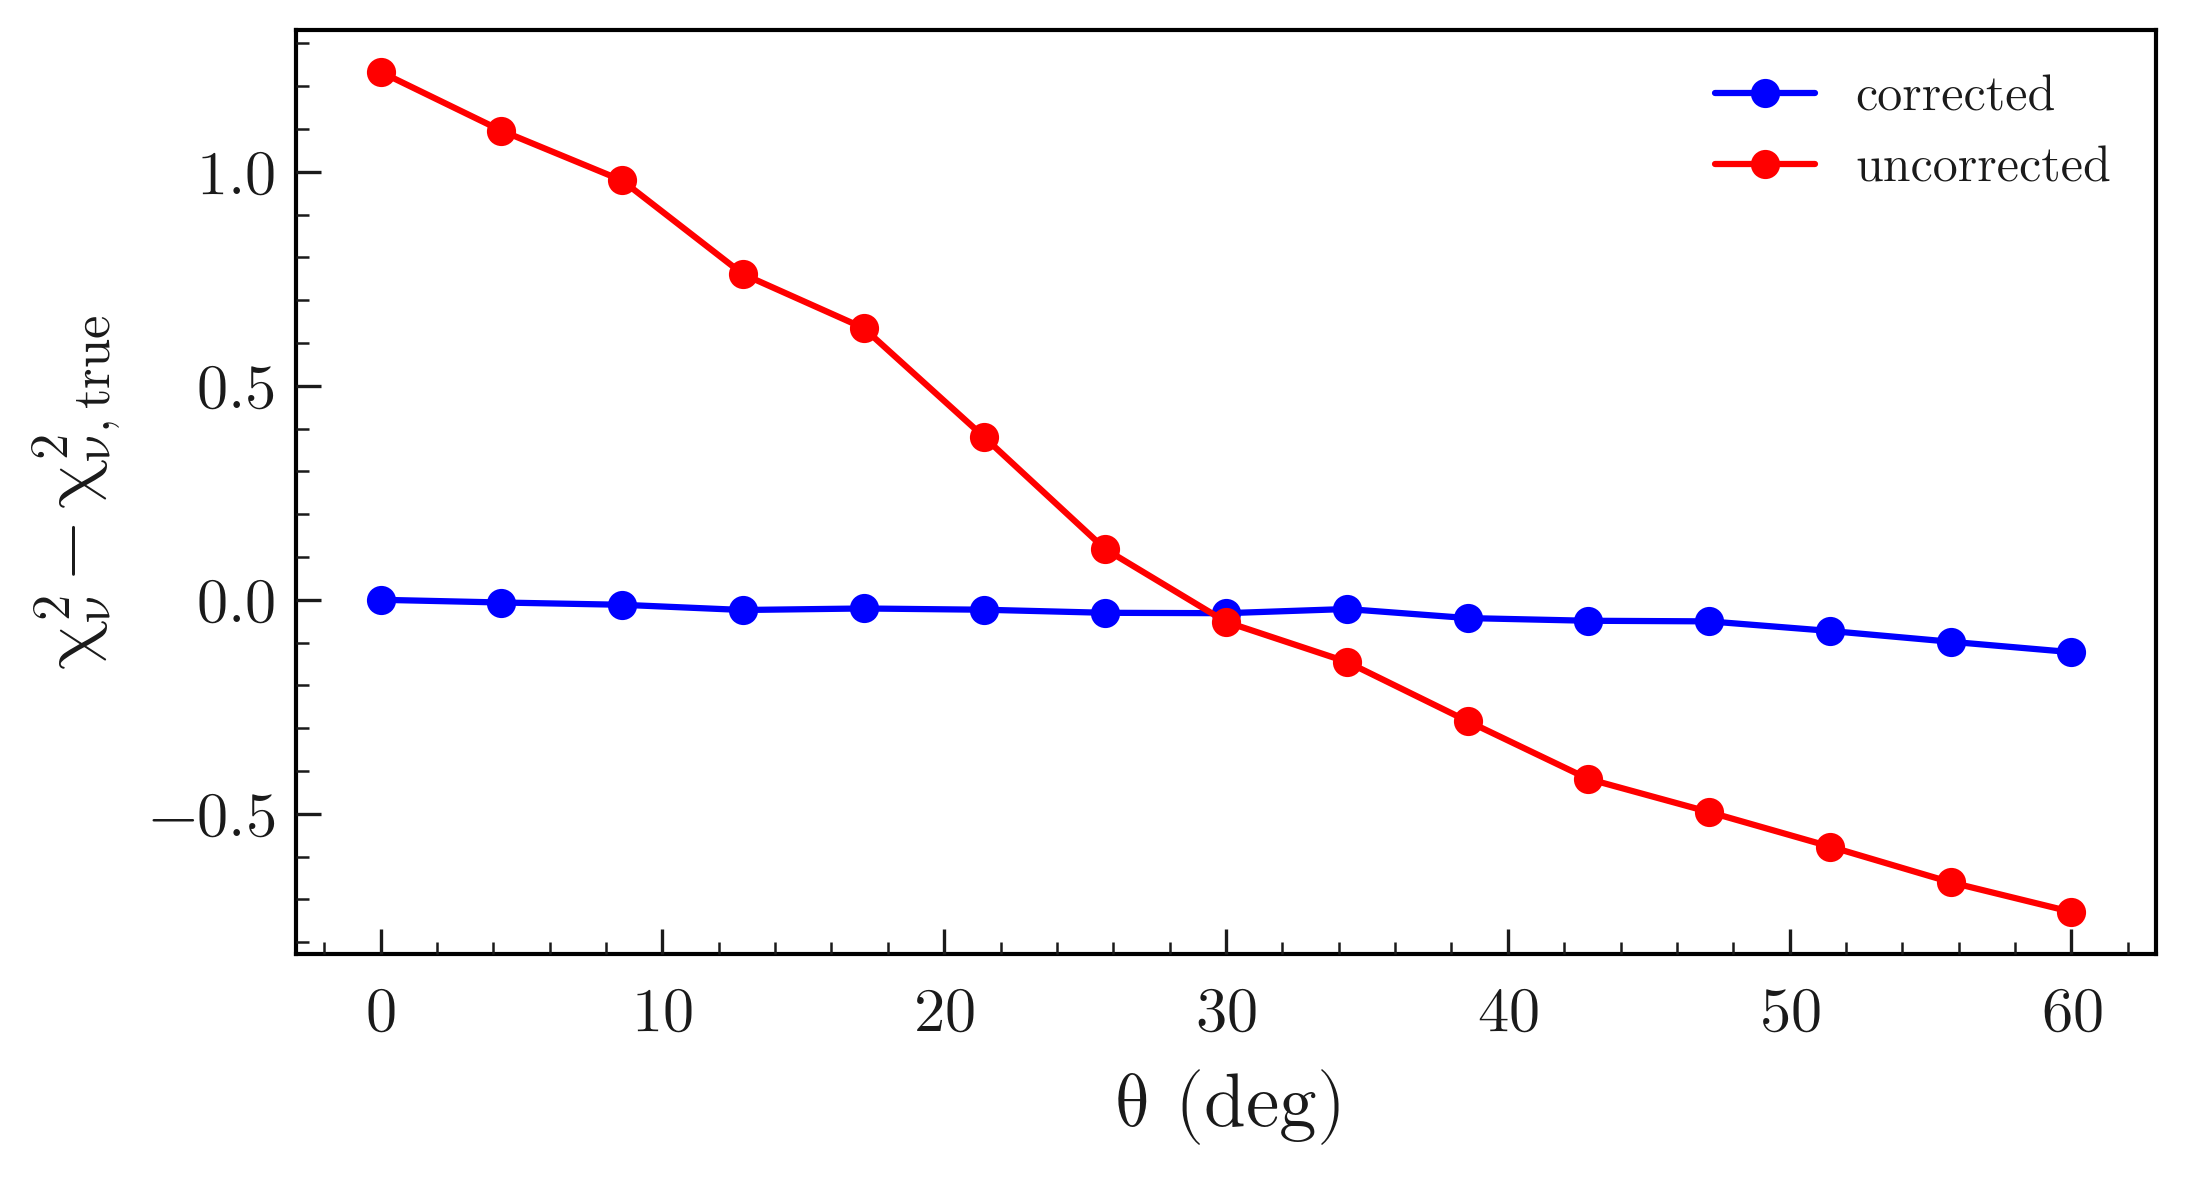
\includegraphics[width=0.6\textwidth]{figs/chi_squared_MW_contribution.png}
    \caption{$\chi^2$ as a function of the Milky Way contribution parameters. The uncorrected line in red is the $\chi^2$ without accounting for the MW contribution on the level of the covariance. The corrected line refers to the $\chi^2$ with accounting for the MW contribution on the level of the covariance.}
    \label{res_fig:mw_chisq}
\end{figure}

\subsection{Host Galaxy Contribution}
The host galaxy contribution is added by sampling from a lognormal distribution with a mean $\mathrm{DM}_\mathrm{host, mean}$ and a lognormal scale $\sigma_\mathrm{LN}$. I vary $\mathrm{DM}_\mathrm{host, mean}$ and study its impact on the mean DM-$z$ relation. The left hand side of Fig. \ref{res_fig:host_dmz_pdf} shows that for large values of $\mathrm{DM}_\mathrm{host, mean}$, the variance of the DM-$z$ relation deviates from the true variance at low redshifts and leads to less deviation at higher redshift. This is due to having a redshift-dependence of the host contribution in the contaminated catalog as in Eq. \ref{eq:dm_host}. The right-hand side plot shows the variation of the PDF with $\mathrm{DM}_\mathrm{host, mean}$. Increasing $\mathrm{DM}_\mathrm{host, mean}$ corresponds to increasing the mean and the variance of the PDF relative to a true catalog without a host contribution.

Fig. \ref{res_fig:host_chisq} shows the variation of $\chi^2$ relative to the value of the reduced fiducial catalog. The red line shows that the $\chi^2$ increases with increasing value of $\mathrm{DM}_\mathrm{host, mean}$ which means that the covariance is underestimated. The blue line corresponds to correcting the covariance matrix by adding the variance as in Eq. \ref{eq:dm_host_cov}. In total, the host contribution leads to biased DM-$z$ relation by larger than 1$\sigma$ and up to 4$\sigma$ depending on $\mathrm{DM}_\mathrm{host, mean}$.

The host contribution model considered in this thesis is motivated by results from analyzing hydrodynamical simulations. Nonetheless, the scatter of $\mathrm{DM}_\mathrm{host}$ in this model is overestimated since the model implicitly marginalizes over the different variables which controls the host contribution such as the halo mass of the host and the position of an FRB in the host.
A more complicated and physically motivated model was introduced by \citet{reischke2024analytical} where the host galaxy contribution is modelled probabilistically, however, with explicit marginalizations over halo masses and the positions of FRBs in the halo. Therefore, future work should explore whether the lognormal model is able to constrain host contribution if the true underlying contribution is sampled from a more complicated model such as the one introduced by \citet{reischke2024analytical}.



\begin{figure}[h!]
    \centering
    \begin{subfigure}[t]{0.48\textwidth}
        \centering
        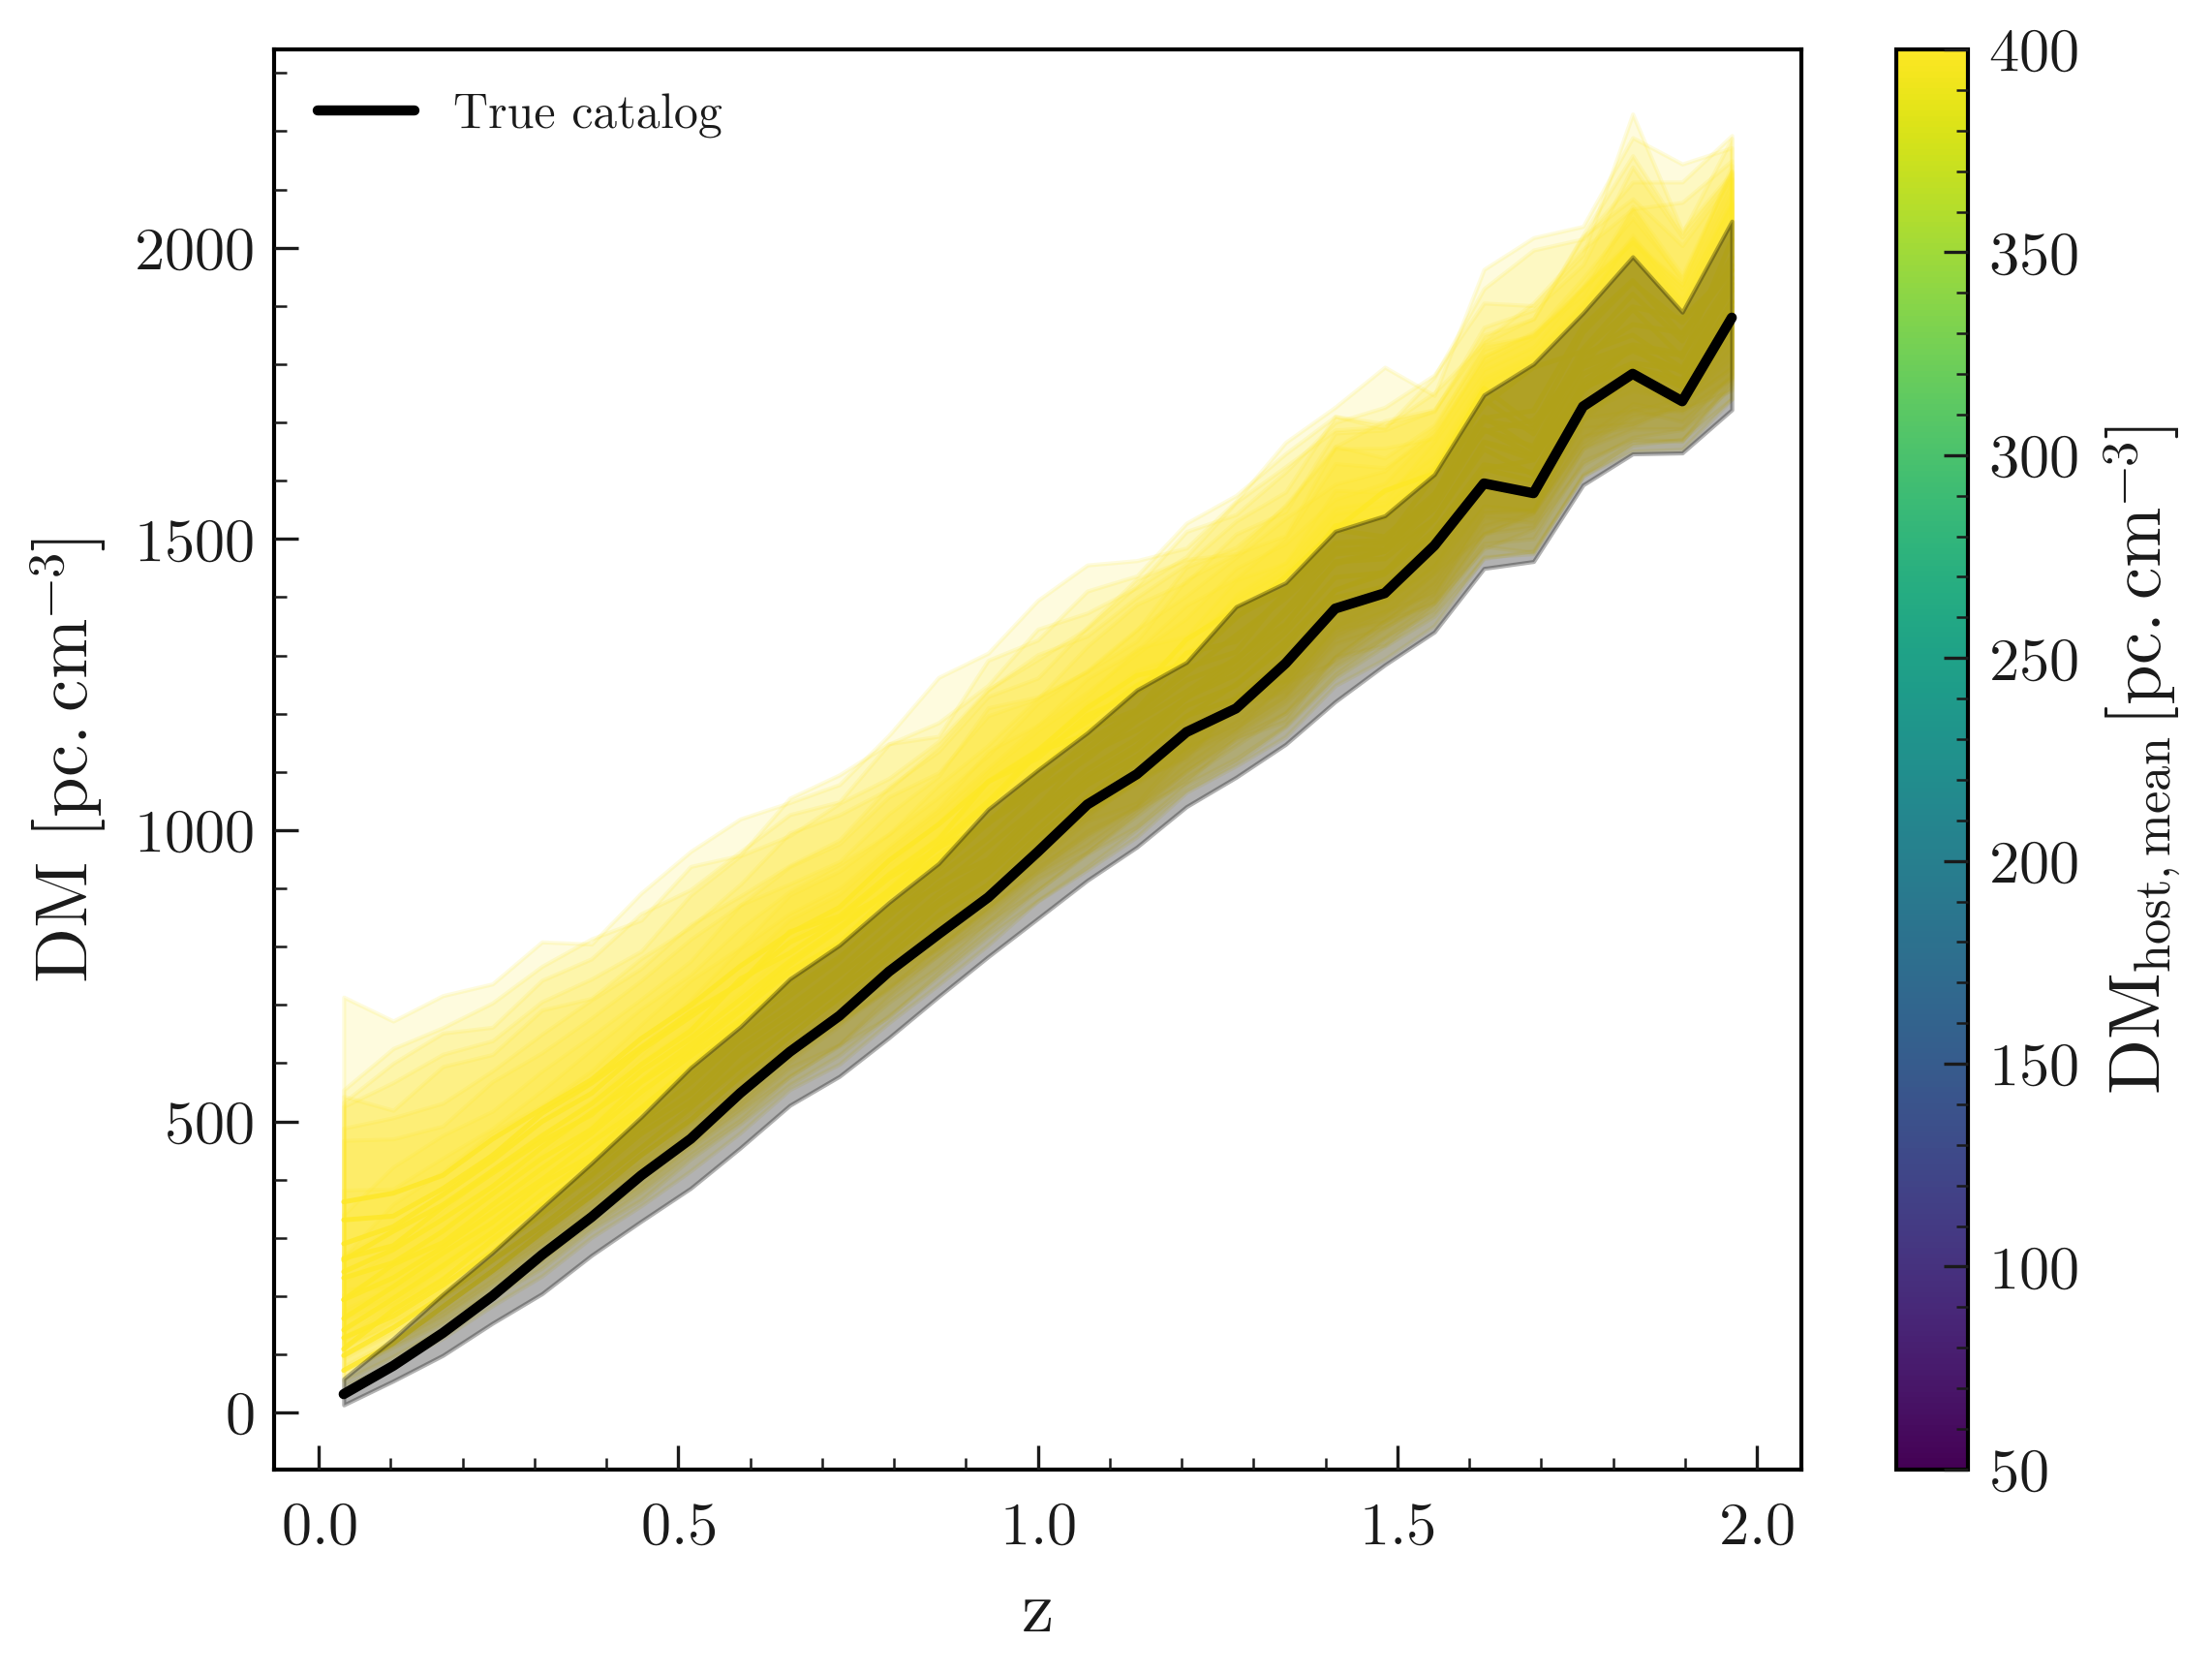
\includegraphics[width=\textwidth]{figs/dm_z_uncertainty_host_contribution.png}
        \caption{DM-$z$ relation for varying host galaxy contribution.}
    \end{subfigure}
    \hfill
    \begin{subfigure}[t]{0.48\textwidth}
        \centering
        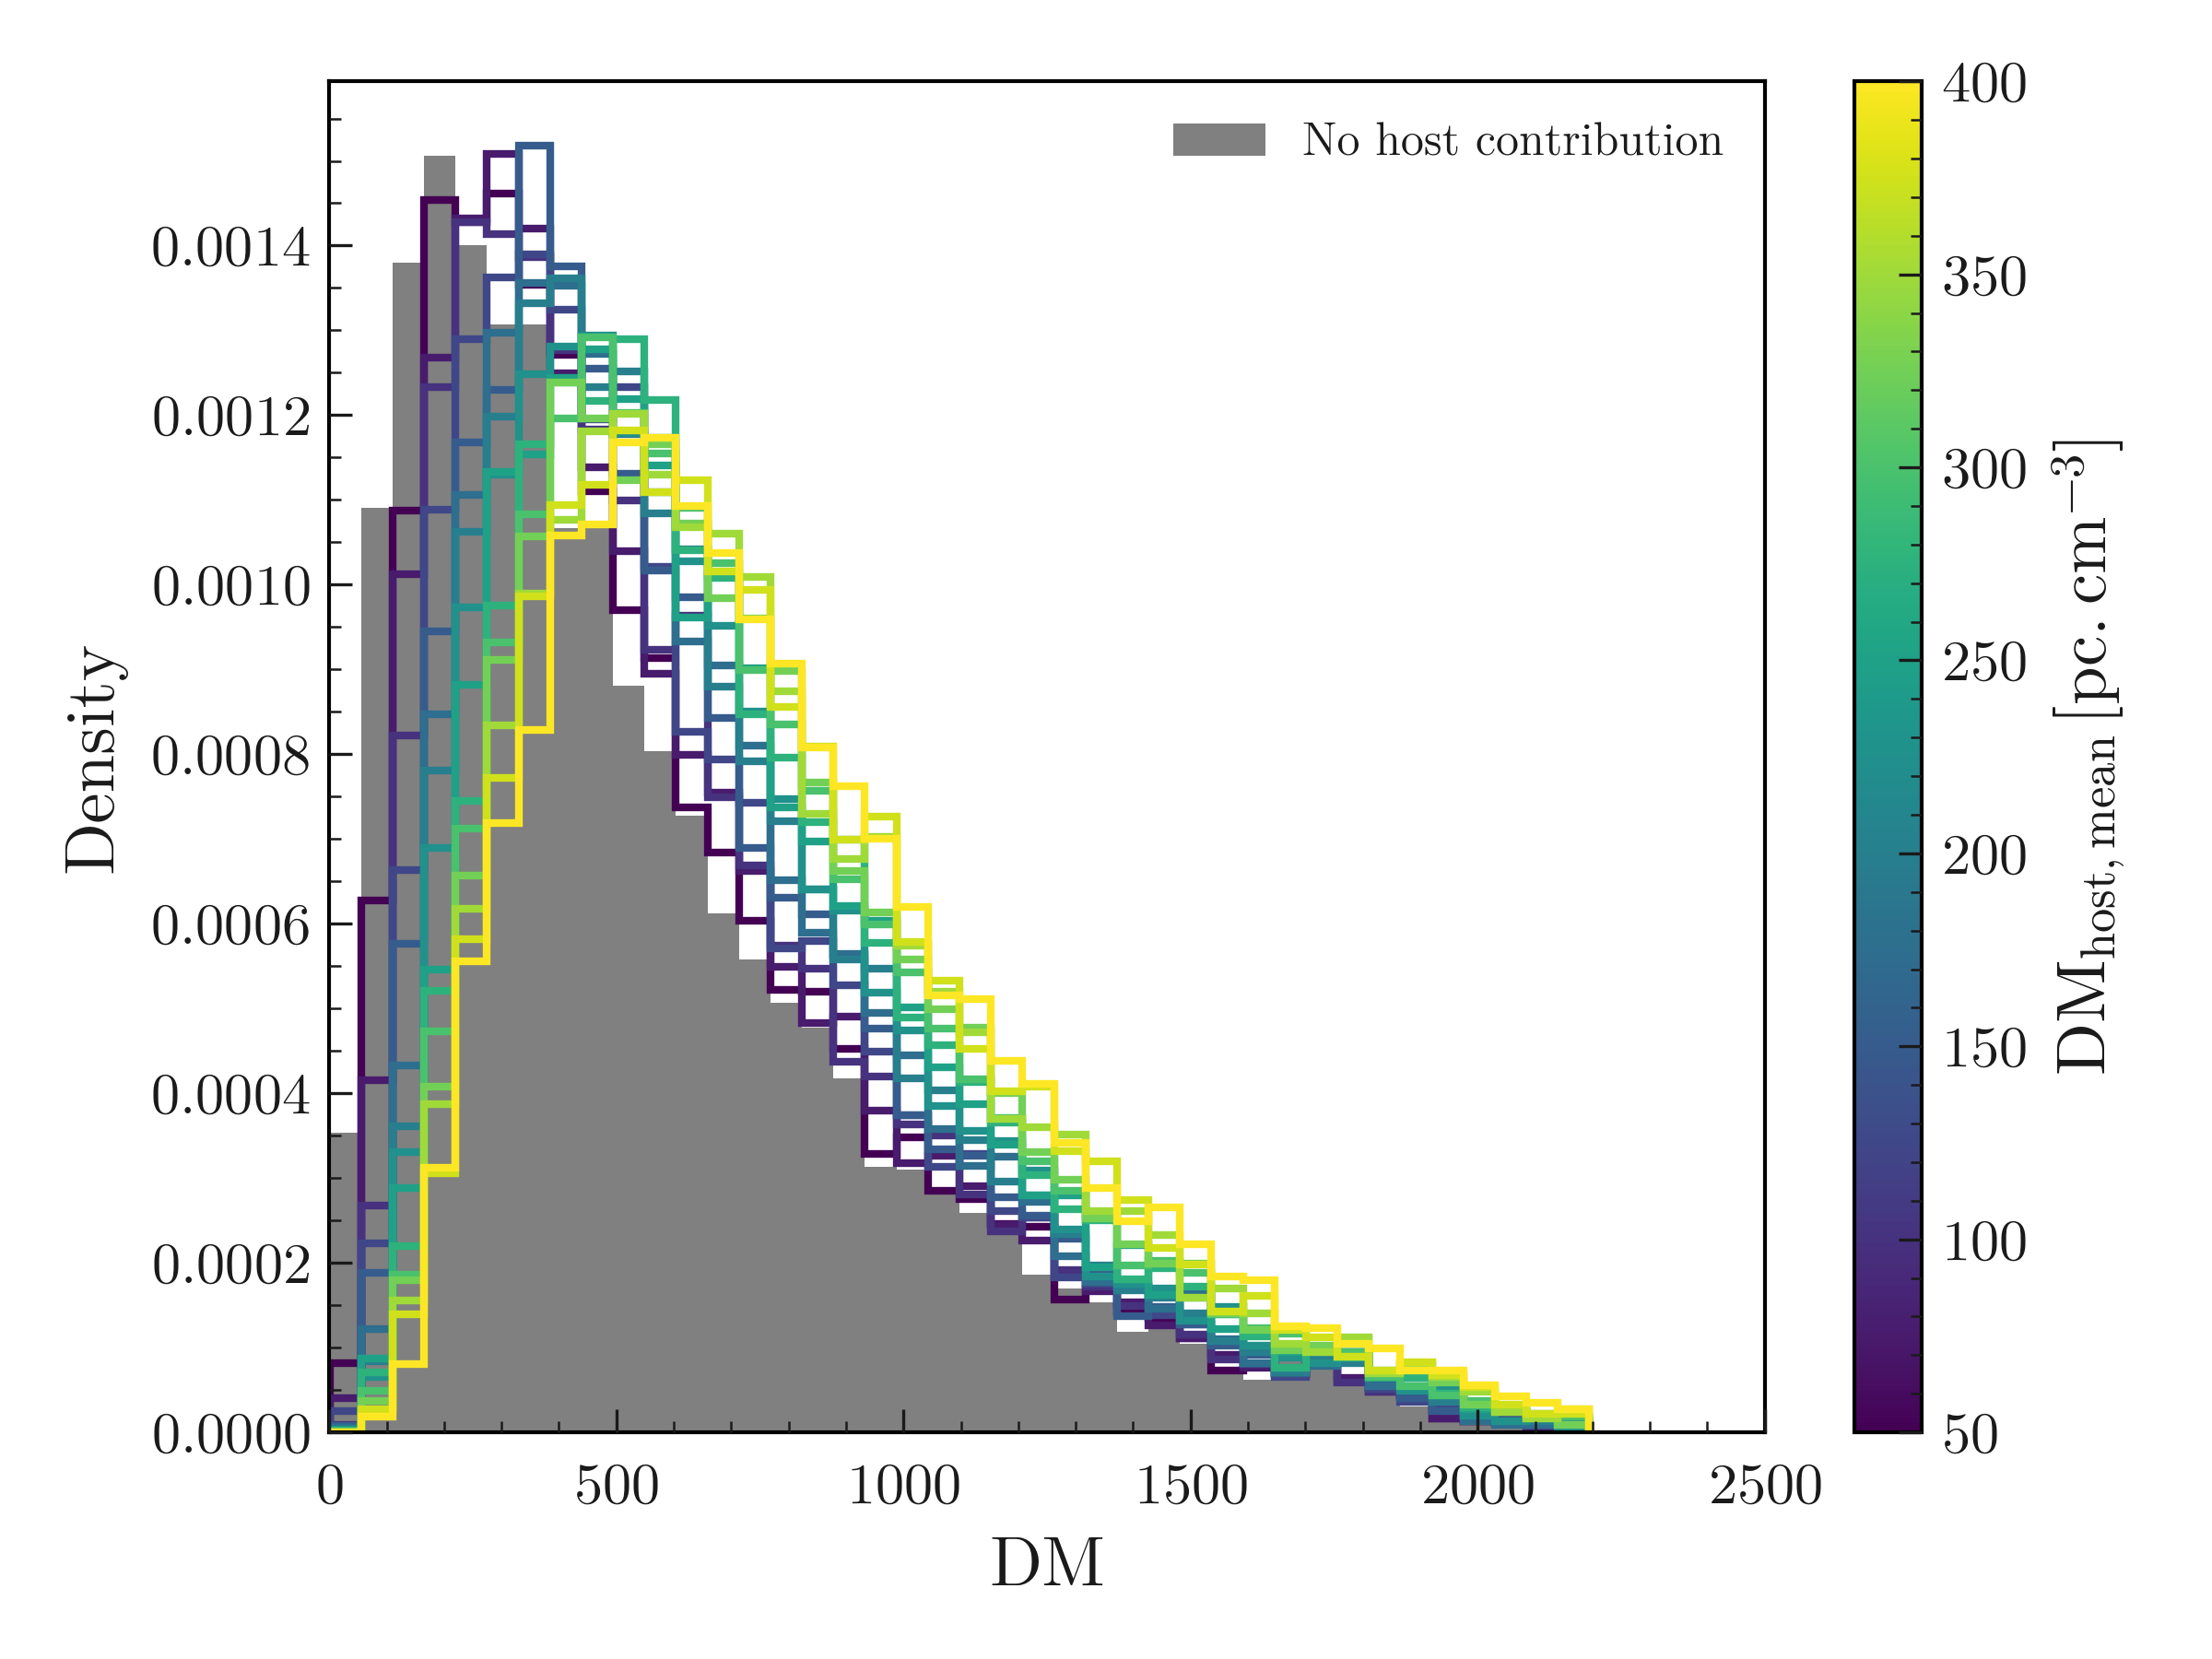
\includegraphics[width=\textwidth]{figs/pdf_uncertainty_host_contribution.png}
        \caption{PDF of DM for varying host galaxy contribution.}
    \end{subfigure}
    \caption{DM-$z$ relation and PDF for the host galaxy contribution systematic.}
    \label{res_fig:host_dmz_pdf}
\end{figure}

\begin{figure}[h!]
    \centering
    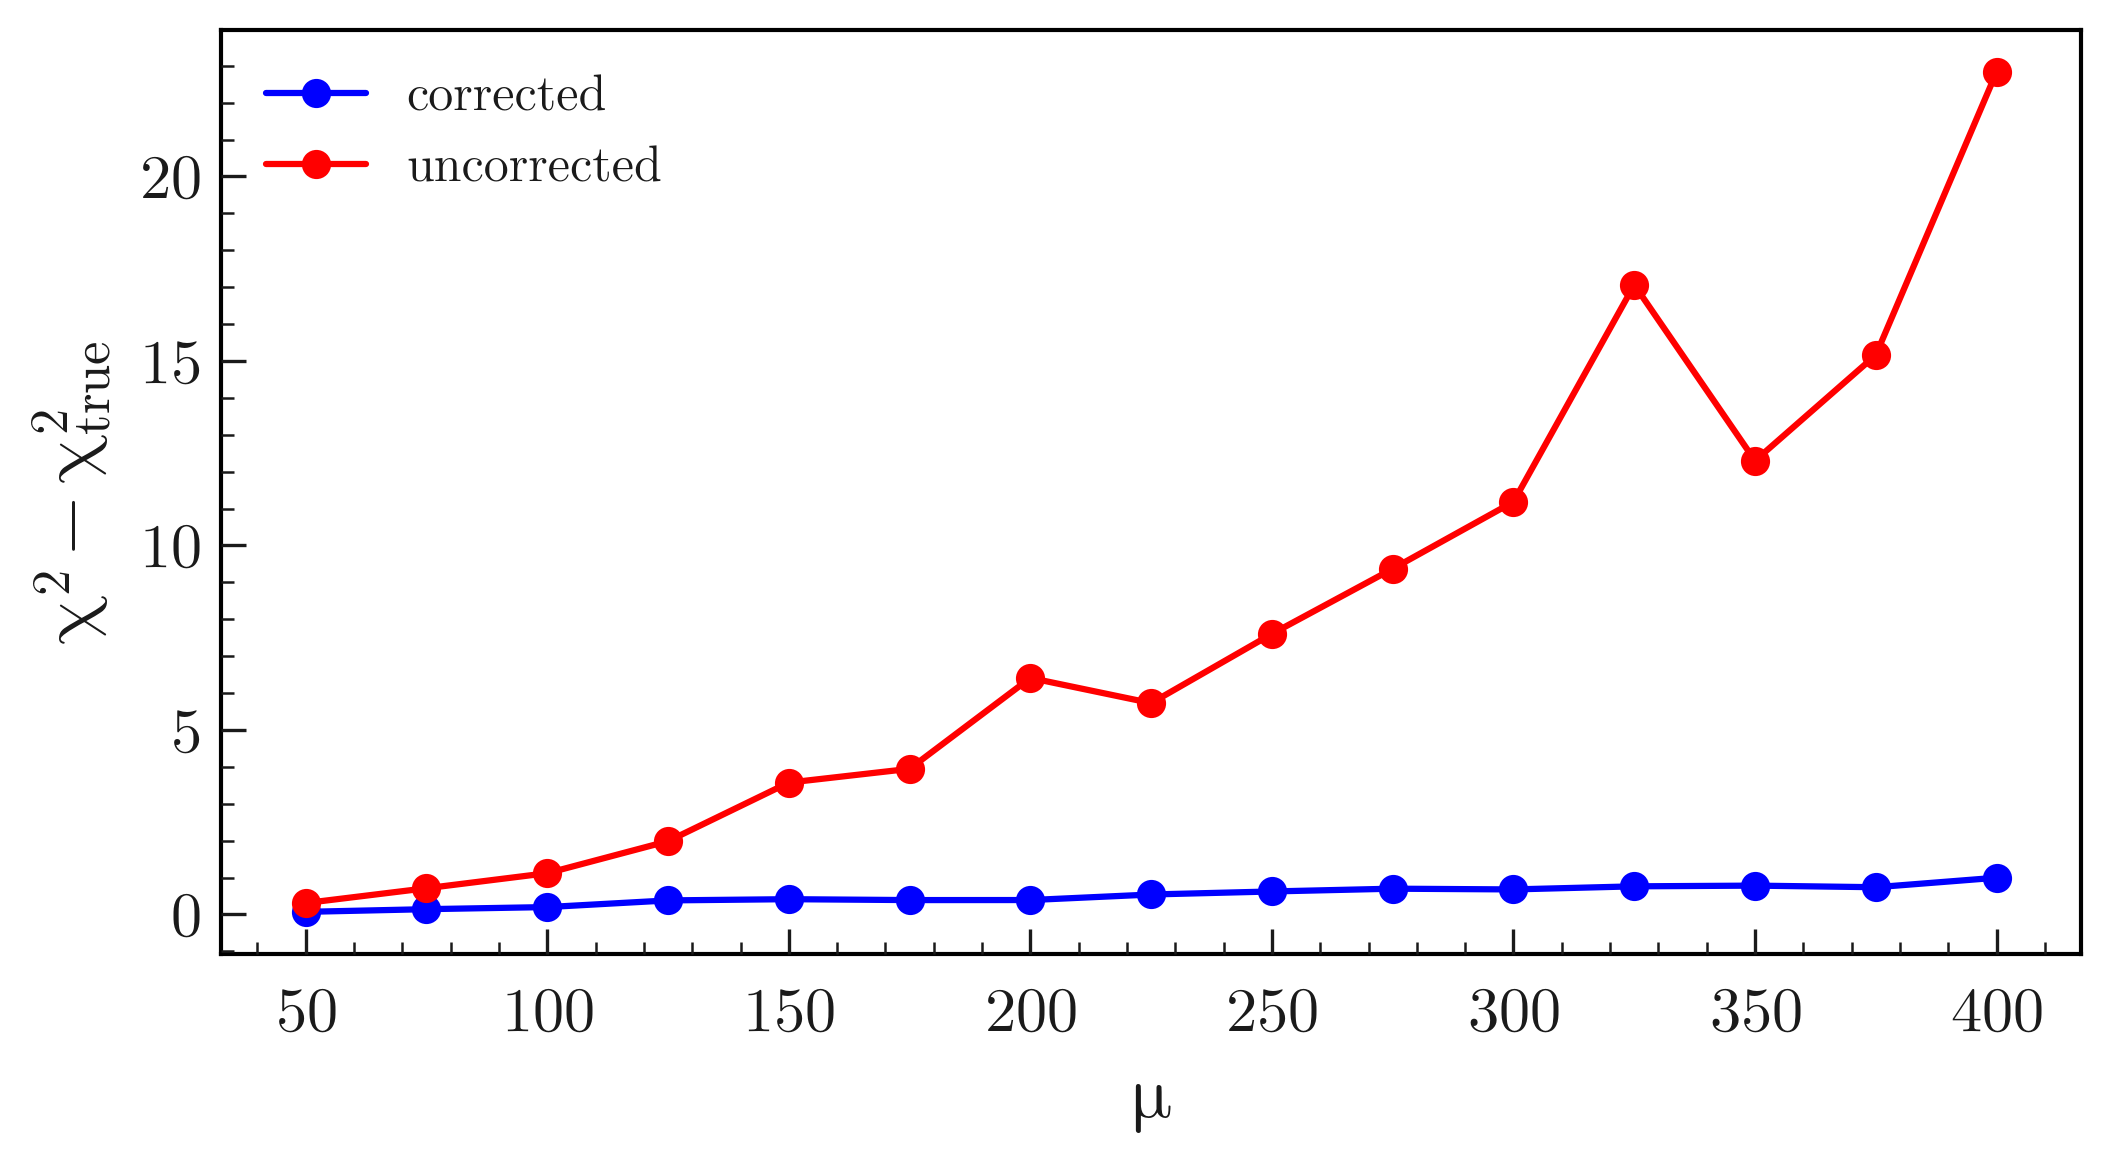
\includegraphics[width=0.6\textwidth]{figs/chi_squared_host_contribution.png}
    \caption{$\chi^2$ as a function of the host galaxy contribution parameters.}
    \label{res_fig:host_chisq}
\end{figure}

\subsection{Redshift Uncertainty}
The impact of redshift uncertainty on the DM-$z$ relation is shown on the left-hand side of Fig. \ref{res_fig:redshift_dmz_pdf}. By increasing the error ratio $\eta$, the mean DM-$z$ relation is consistent with the mean DM-$z$ relation for low values of $\eta$ with only the variance getting larger than that of the true catalog. For larger $\eta$, both the mean and variance are different from the true catalog. This is further reflected in the right-hand side of Fig. \ref{res_fig:redshift_dmz_pdf} where the variance of the PDF increases with increasing $\eta$ while the peak of the distribution shifts to the left, corresponding to a lower mean.




\begin{figure}[h!]
    \centering
    \begin{subfigure}[t]{0.48\textwidth}
        \centering
        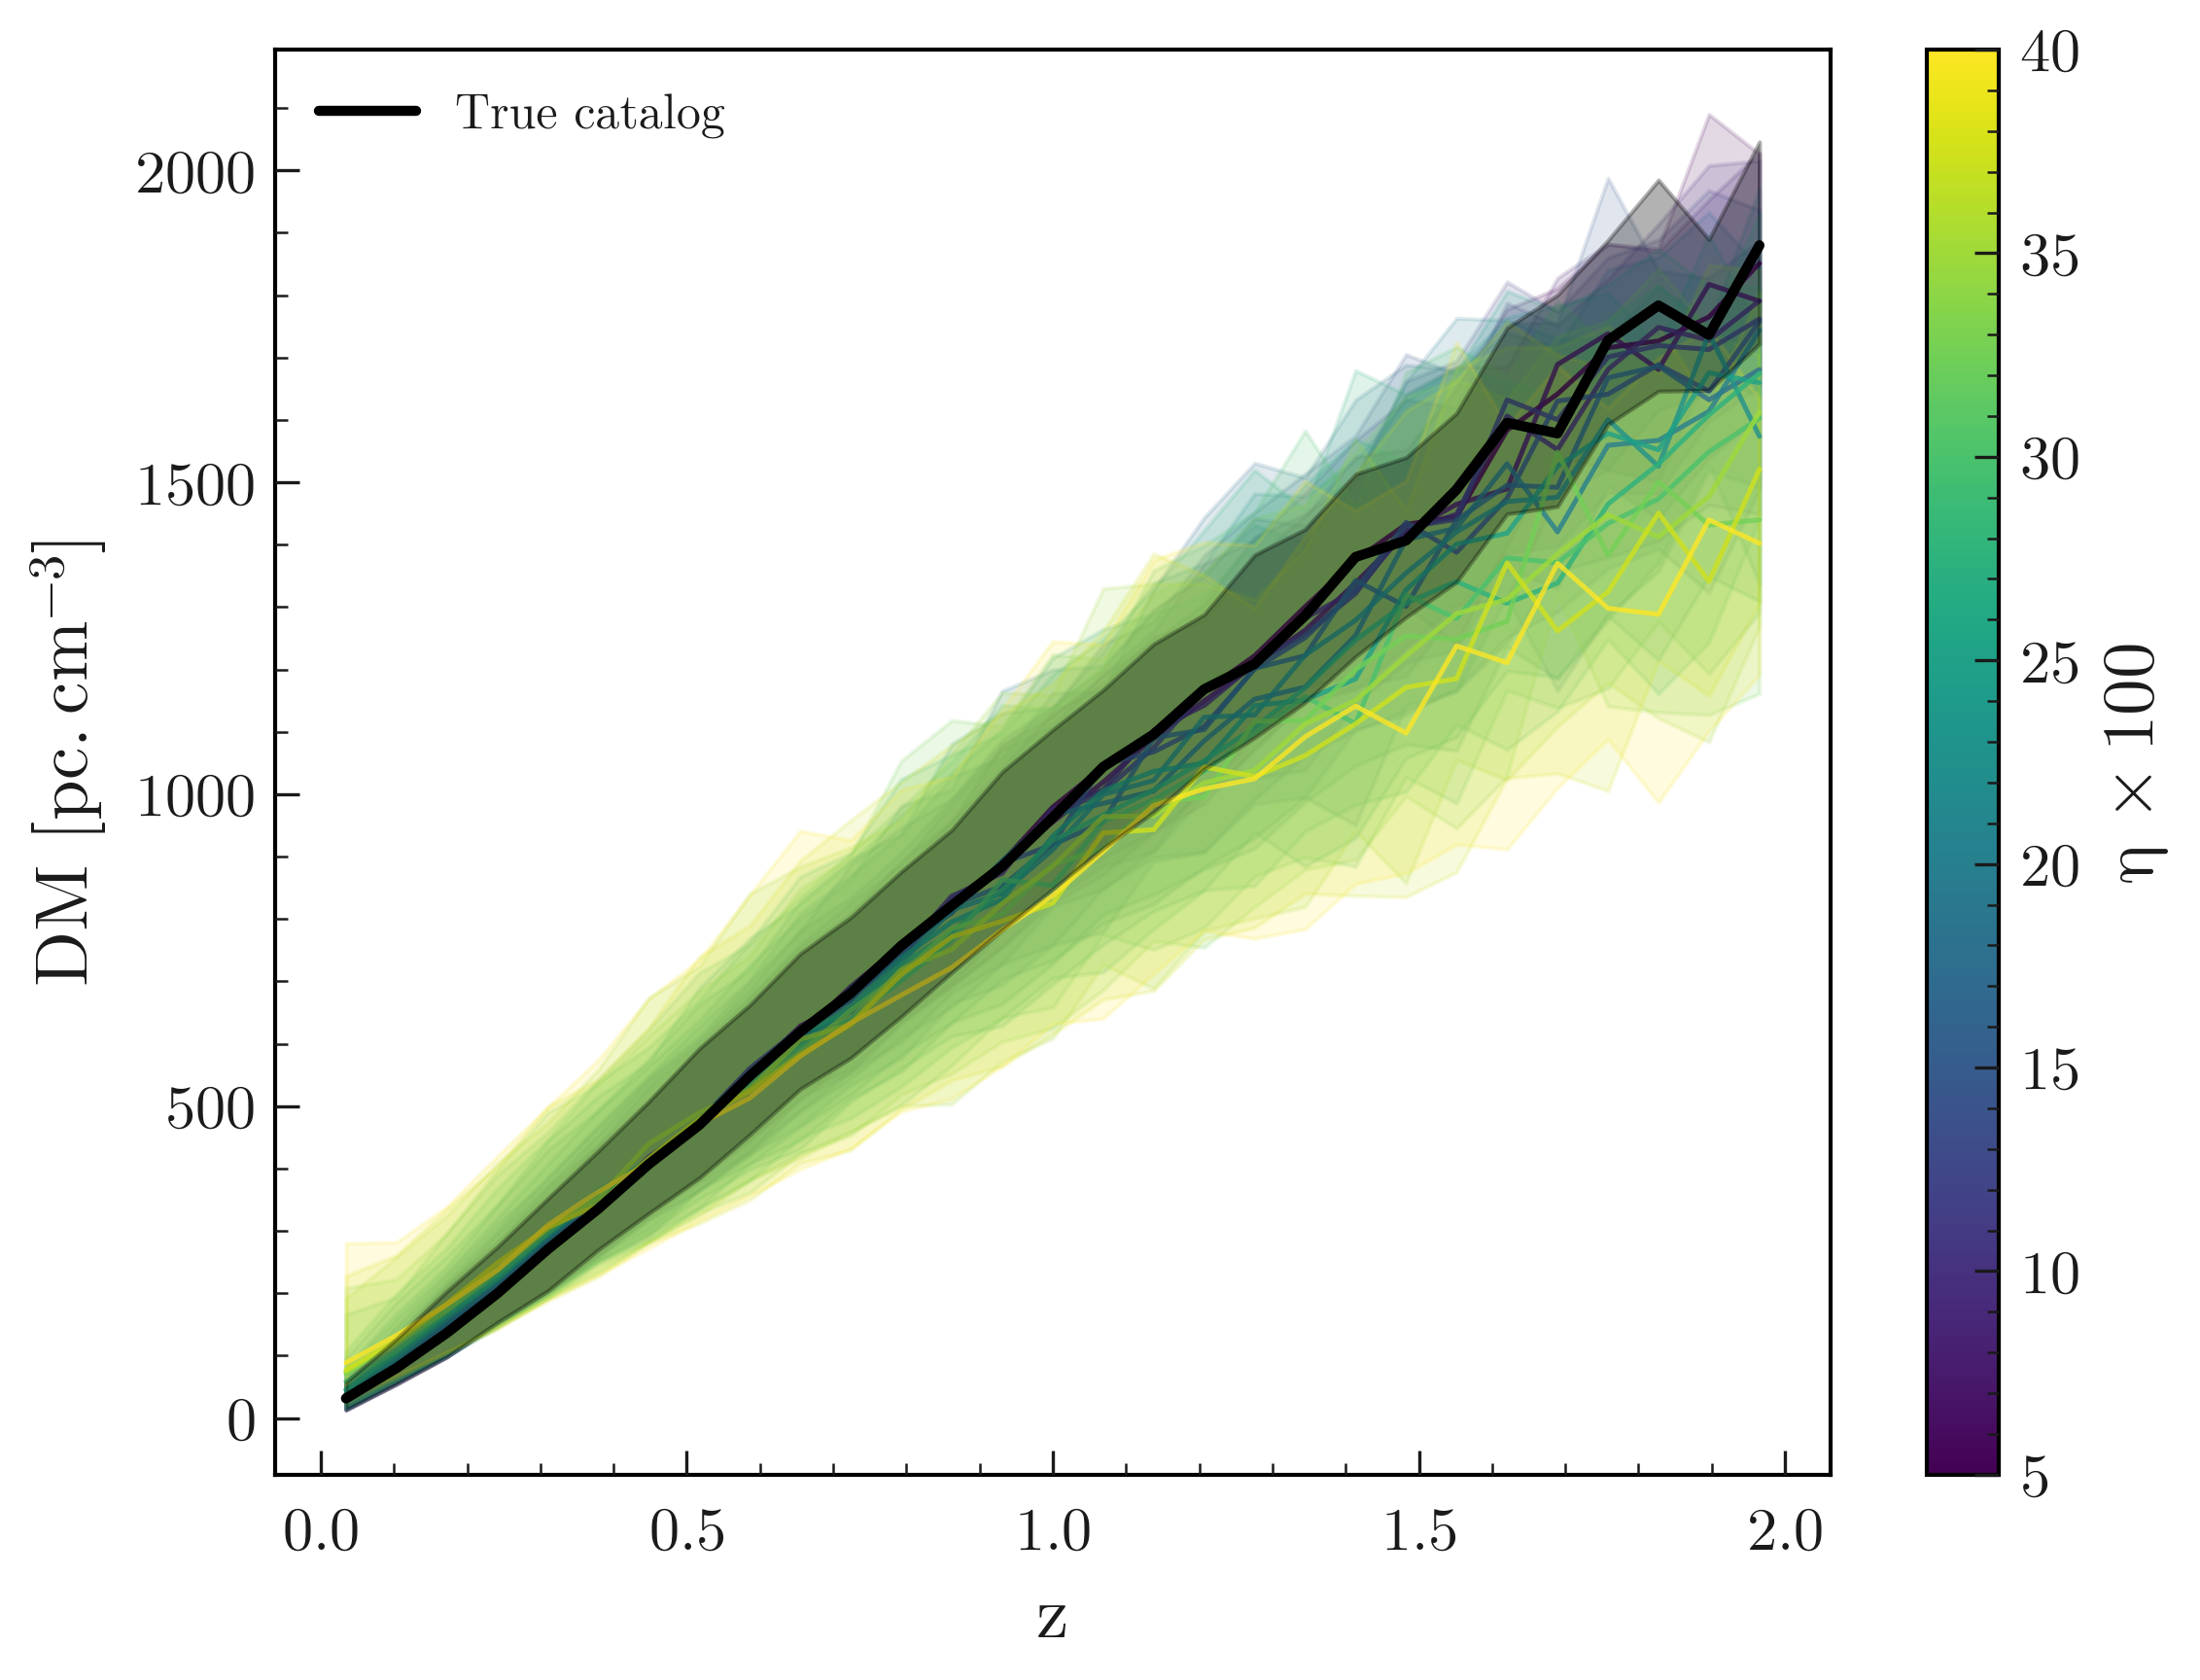
\includegraphics[width=\textwidth]{figs/dm_z_uncertainty_z_uncertainty.png}
        \caption{DM-$z$ relation for varying redshift uncertainty.}
    \end{subfigure}
    \hfill
    \begin{subfigure}[t]{0.48\textwidth}
        \centering
        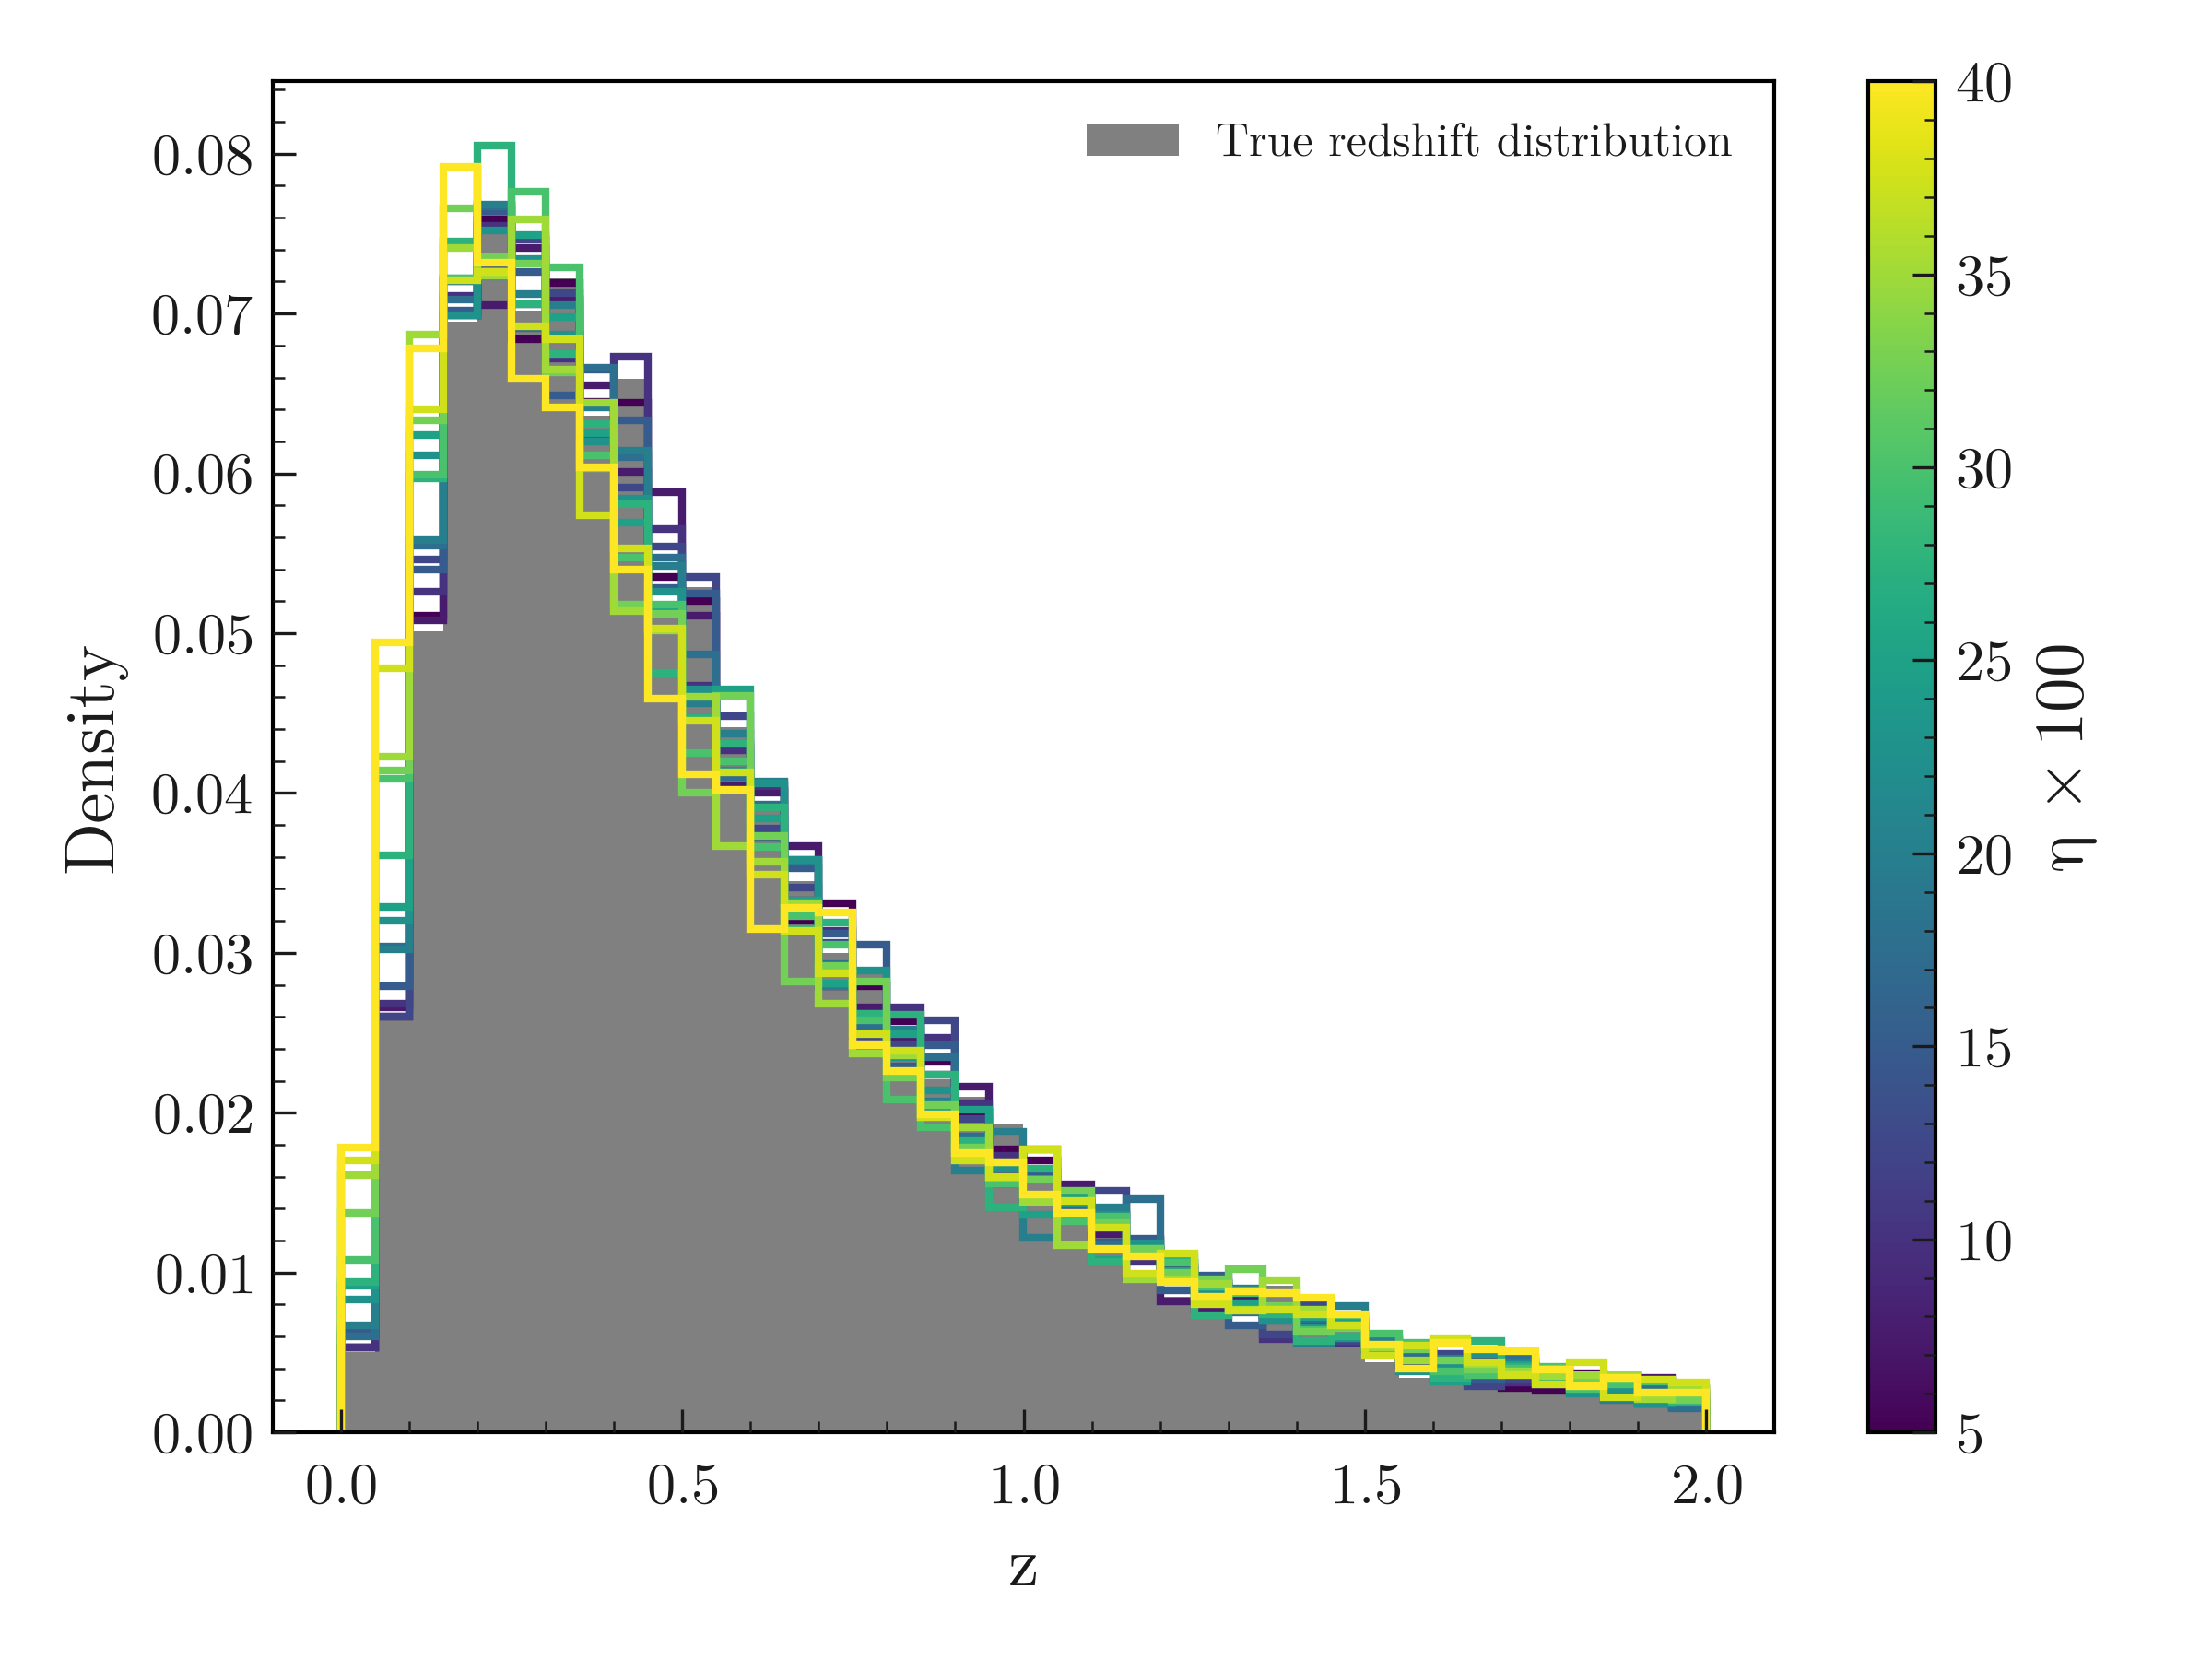
\includegraphics[width=\textwidth]{figs/pdf_uncertainty_z_uncertainty.png}
        \caption{PDF of DM for varying redshift uncertainty.}
    \end{subfigure}
    \caption{DM-$z$ relation and PDF for the redshift uncertainty systematic.}
    \label{res_fig:redshift_dmz_pdf}
\end{figure}




The deviation in $\chi^2$ is shown in Fig. \ref{res_fig:redshift_chisq}. The corrected line corresponds to propagating the error to the covariance as described by Eq. \ref{eq:cov_z_uncertainty}. Meanwhile, the deviation from the fiducial catalog crosses the 1$\sigma$ level for $\eta \approx 15\%$ and gets up to $4.5\sigma$ for $\eta \approx 35\%$. The $\chi^2$ decreases afterwards since the corresponding mean DM-$z$ of the contaminated catalog decreases. Therefore, for a simple scenario of redshift uncertainty, accounting for the redshift uncertainty is important to constrain the DM-$z$ relation and the corresponding parameters.

The redshift uncertainty model discussed in this thesis is a simple model of uncertainty which assumes symmetric error. In other scenarios, it is possible that the redshift error is asymmetric, and the error propagation in this case is nontrivial. Nonetheless, with the simulation based approach, it is possible to integrate any scenario of redshift uncertainty. This is a crucial property when solving inference problem with FRBs detected by different surveys and localised in different methods.

As mentioned in section \ref{theory_sec:uncertainties}, it is possible to localise FRBs by comparing their galactic coordinates with wide galaxy surveys to find possible candidates for a host galaxy with each host candidate having a certain probability to be the host. In this case, propagating the error is not a trivial task either and the redshift uncertainty can be simulated as being sampled from a weighted sum of Gaussian distributions where each distribution represents a candidate for a host galaxy.




\begin{figure}[h!]
    \centering
    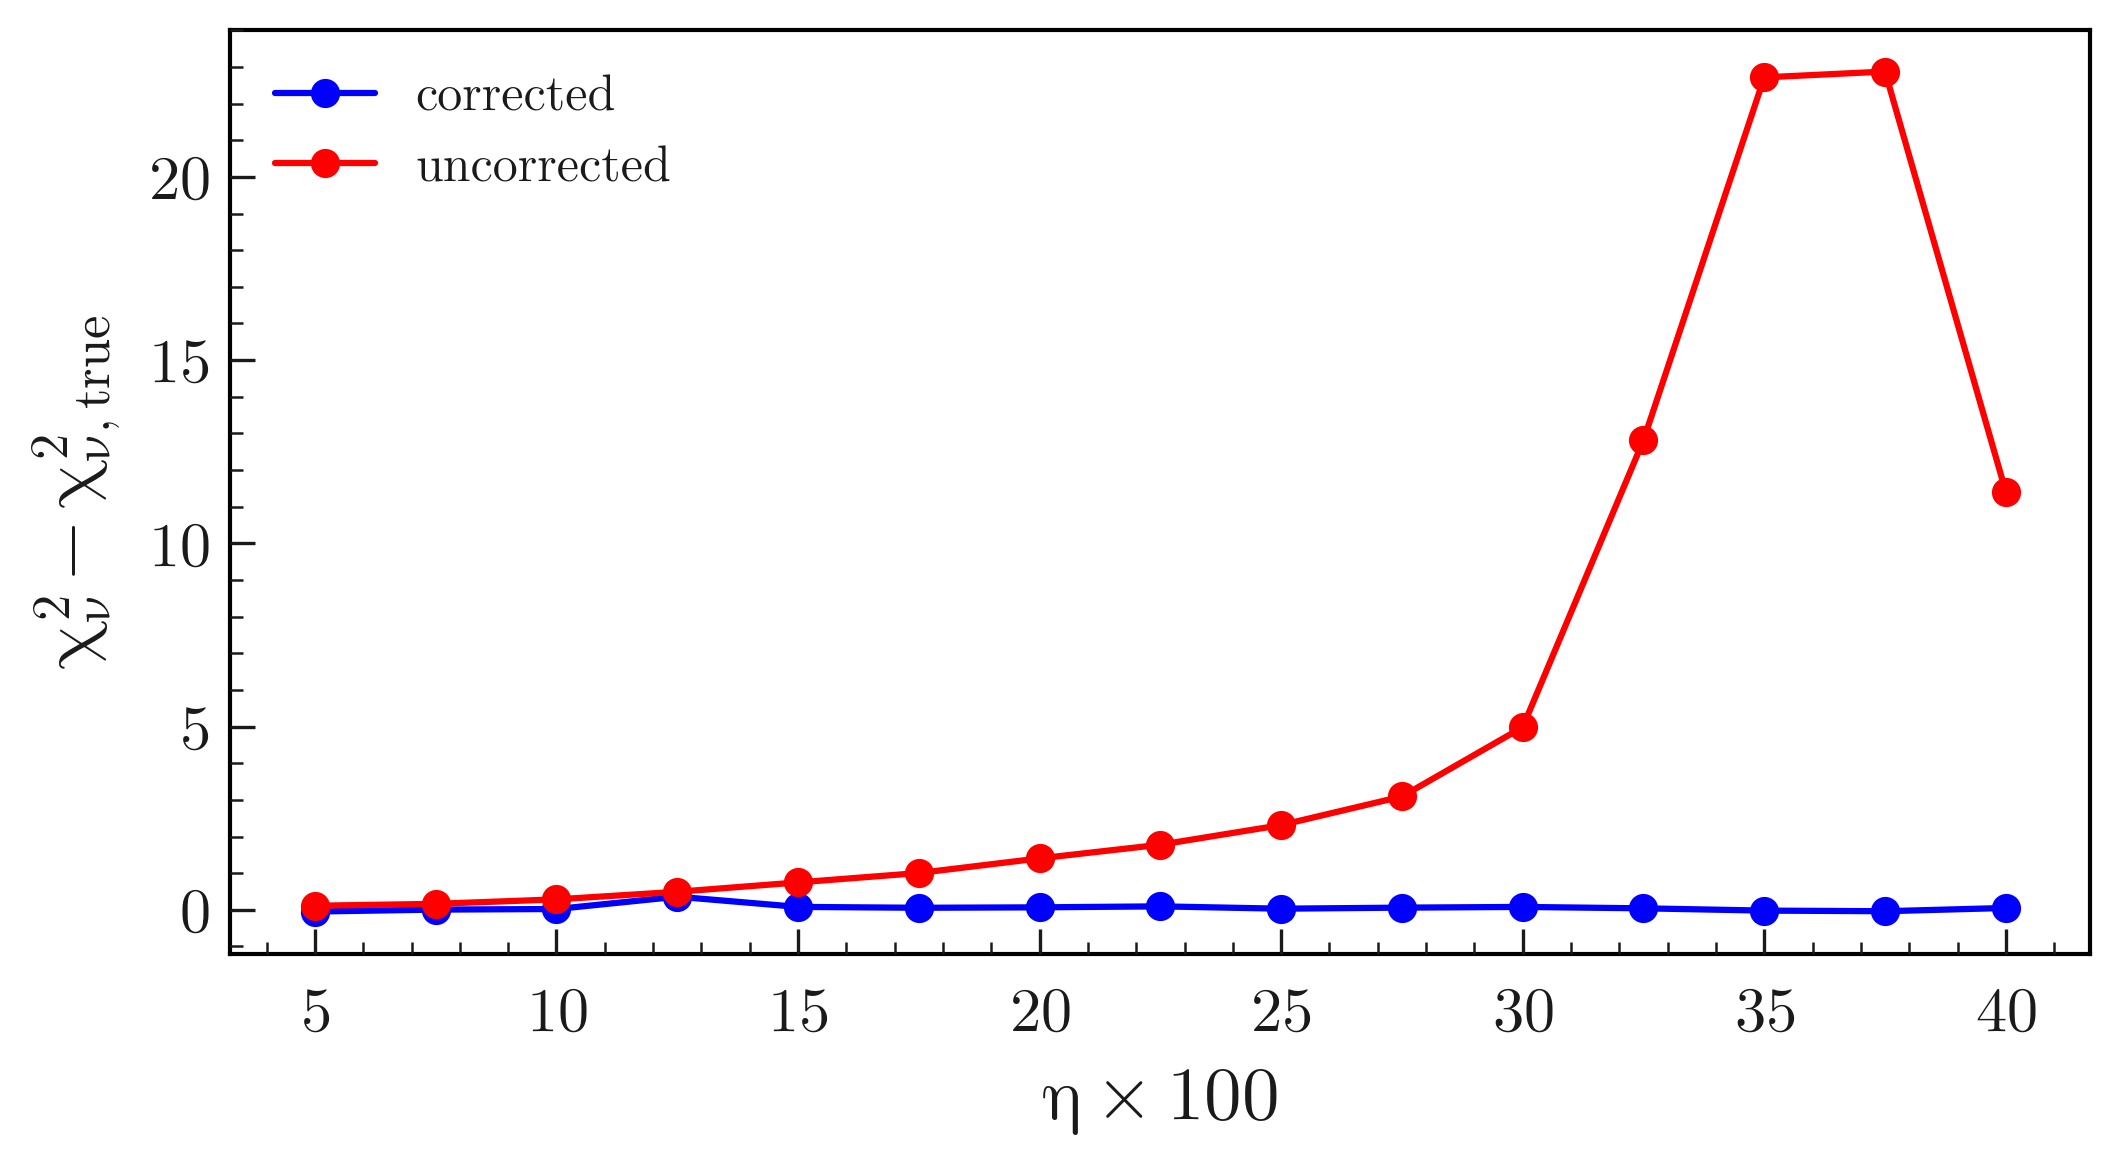
\includegraphics[width=0.6\textwidth]{figs/chi_squared_z_uncertainty.png}
    \caption{$\chi^2$ as a function of the redshift uncertainty parameter $\eta$.}
    \label{res_fig:redshift_chisq}
\end{figure}

\subsection{Selection Effects}
Fig. \ref{res_fig:selection_dmz_pdf} shows the impact of reweighting the PDF with a sigmoid function that represents the telescope selection effects. The sigmoid function modifies the shape of the PDF at large values of DM in addition to changing the normalisation. The impact is negligible for larger values of $\mathrm{DM}_\mathrm{max}$ since the range of DM values considered in this work are below $\mathrm{DM} \approx 2000 \mathrm{pc.cm}^{-3}$ since the simulation is limited to sources up to redshifts 2.




\begin{figure}[h!]
    \centering
    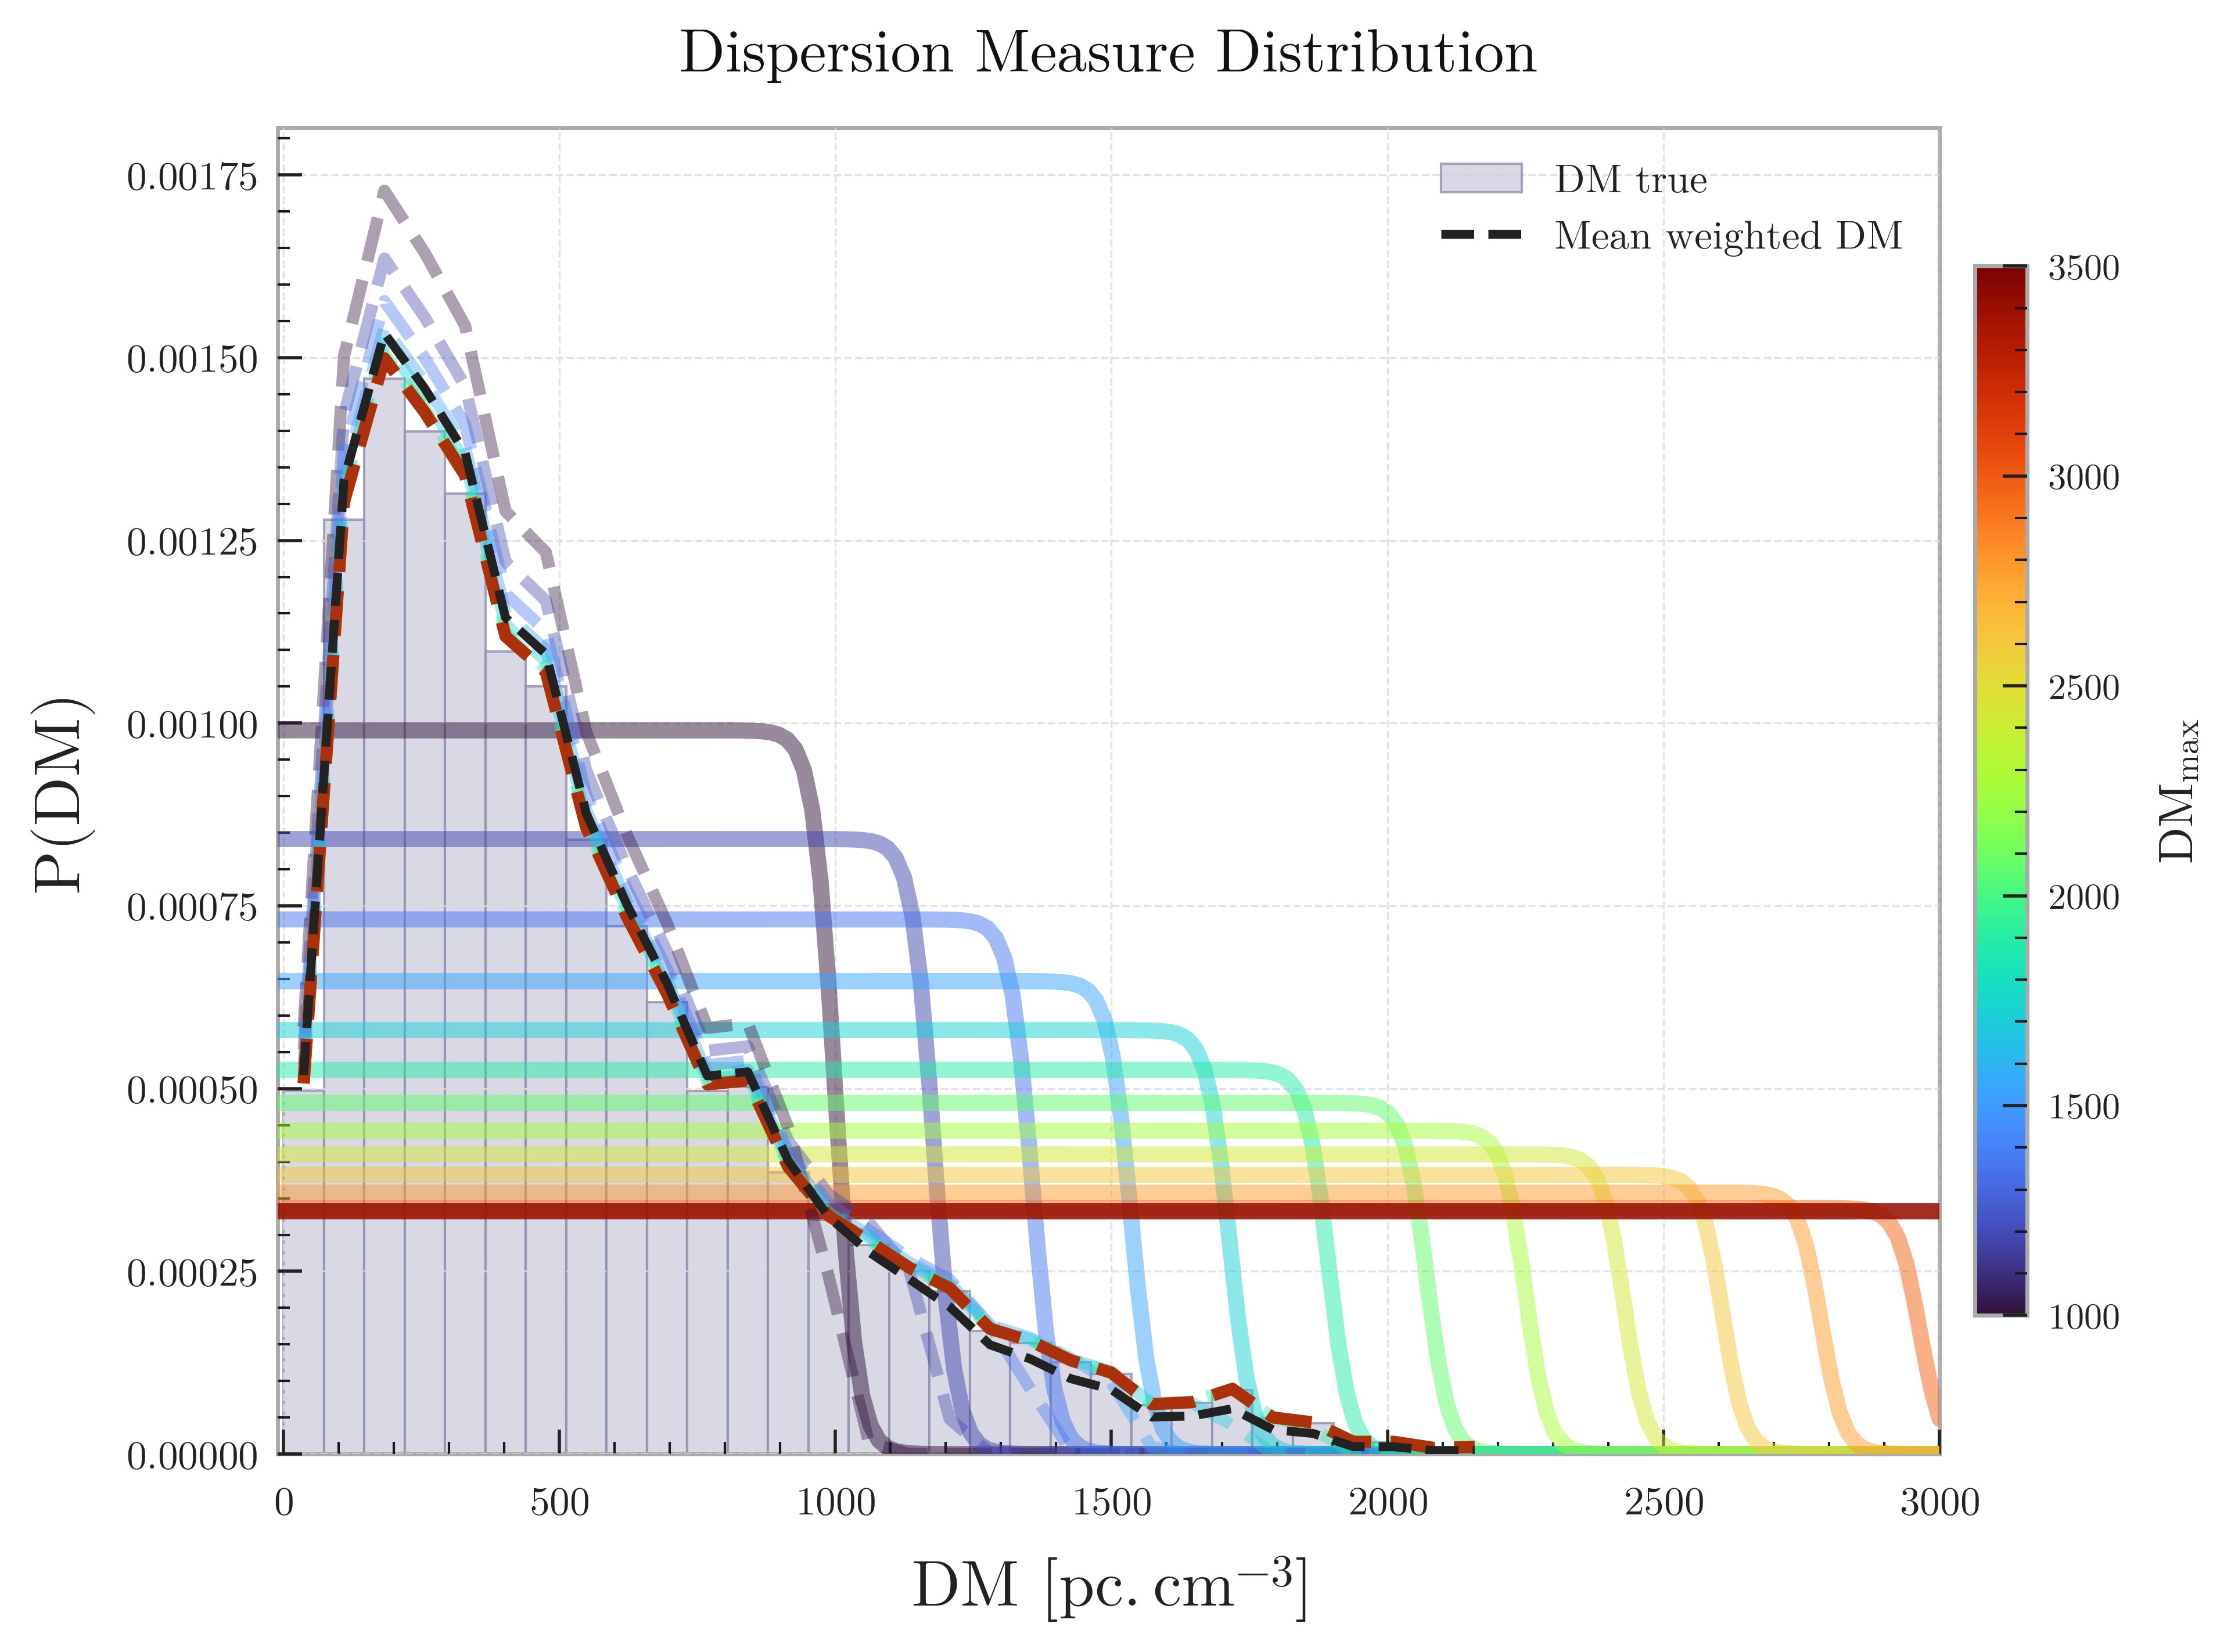
\includegraphics[width=0.7\textwidth]{figs/pdf_DM_max_selection_effects.png}
    \caption{PDF of DM for varying selection effect parameters.}
    \label{res_fig:selection_dmz_pdf}
\end{figure}

As a consequence, the $\chi^2$ shown in Fig. \ref{res_fig:selection_chisq} shows less than 1$\sigma$ deviation from the true catalog. By considering sources at higher redshift this effect has more impact on the inferred DM-$z$ relation. Furthermore, I have limited the study to the expected source-redshift distribution expected for the SKOA, however, for a full cosmological analysis the source redshift distribution is modelled and parameterized. The parameters are freed and then marginalized to obtain constraints on the cosmological parameters \citep{hoyle2018dark}.


\begin{figure}[h!]
    \centering
    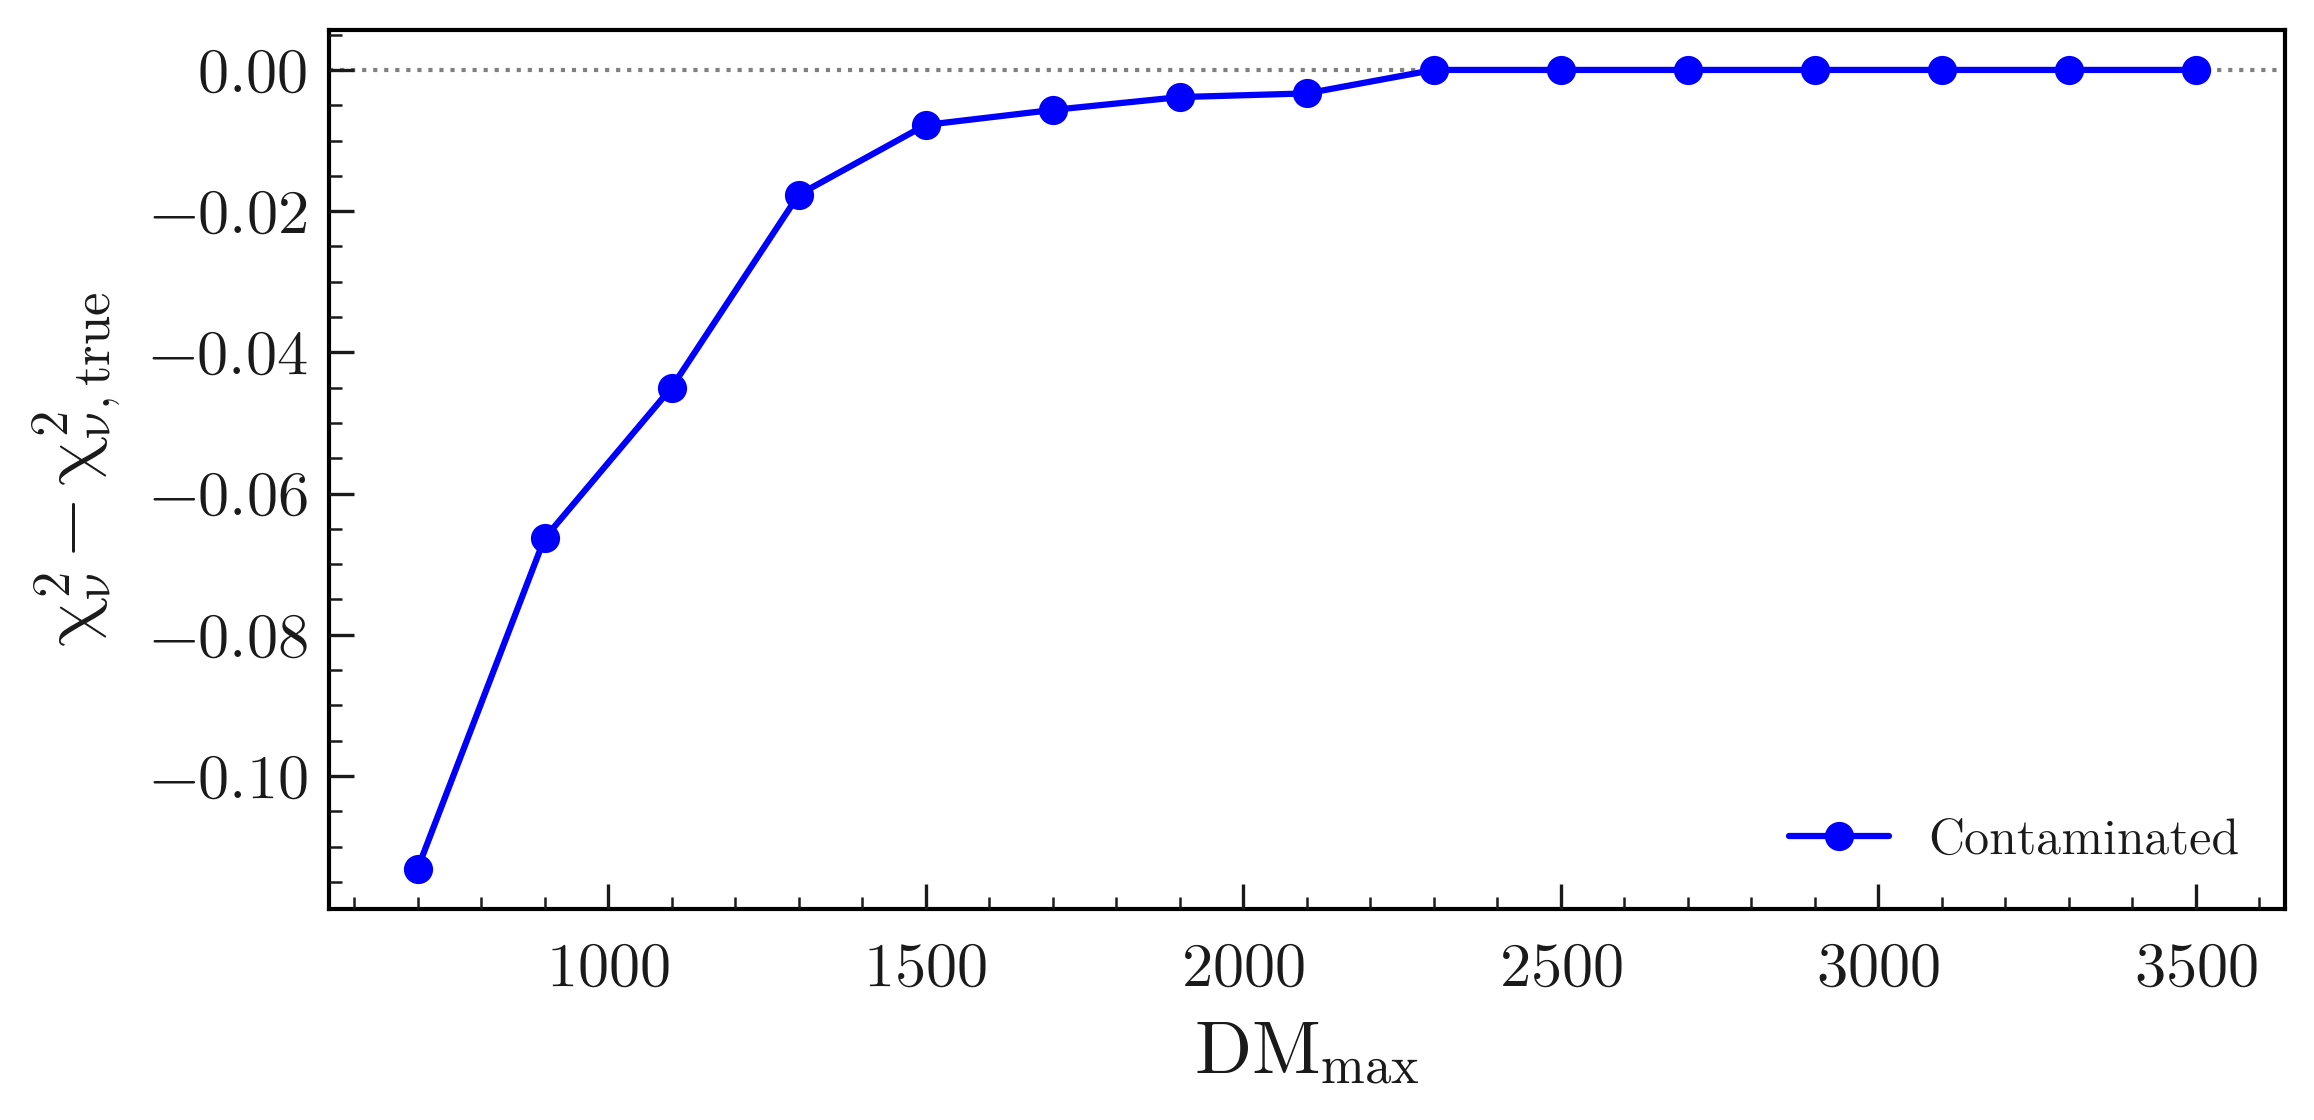
\includegraphics[width=0.6\textwidth]{figs/chi_squared_selection_effects.png}
    \caption{$\chi^2$ as a function of the selection effect parameters ($\mathrm{DM}_\mathrm{max}$, $\epsilon$).}
    \label{res_fig:selection_chisq}
\end{figure}

\subsection{Unlocalised Hosts}
In this section, I present the impact of using unlocalised FRBs in a cosmological analysis for three cases: randomly missing redshifts, a fraction of high redshift sources is missing, and a fraction of low redshift sources is missing.


% --- Random subset ---
The left-hand side of Fig \ref{res_fig:unloc_random_dmz_pdf} shows the resulting DM-$z$ relation for a varied fraction of unlocalised FRBs $f$. The mean DM-$z$ relation is consistent with that of the true catalog, but the variance is larger than the true catalog for the entire range of $f$ at higher redshifts. The PDF displayed on the right-hand side of Fig. \ref{res_fig:unloc_random_dmz_pdf} shows a slight change in the width of the PDF which is reflected by the change in the variance of the DM-$z$ relation.




\begin{figure}[h!]
    \centering
    \begin{subfigure}[t]{0.48\textwidth}
        \centering
        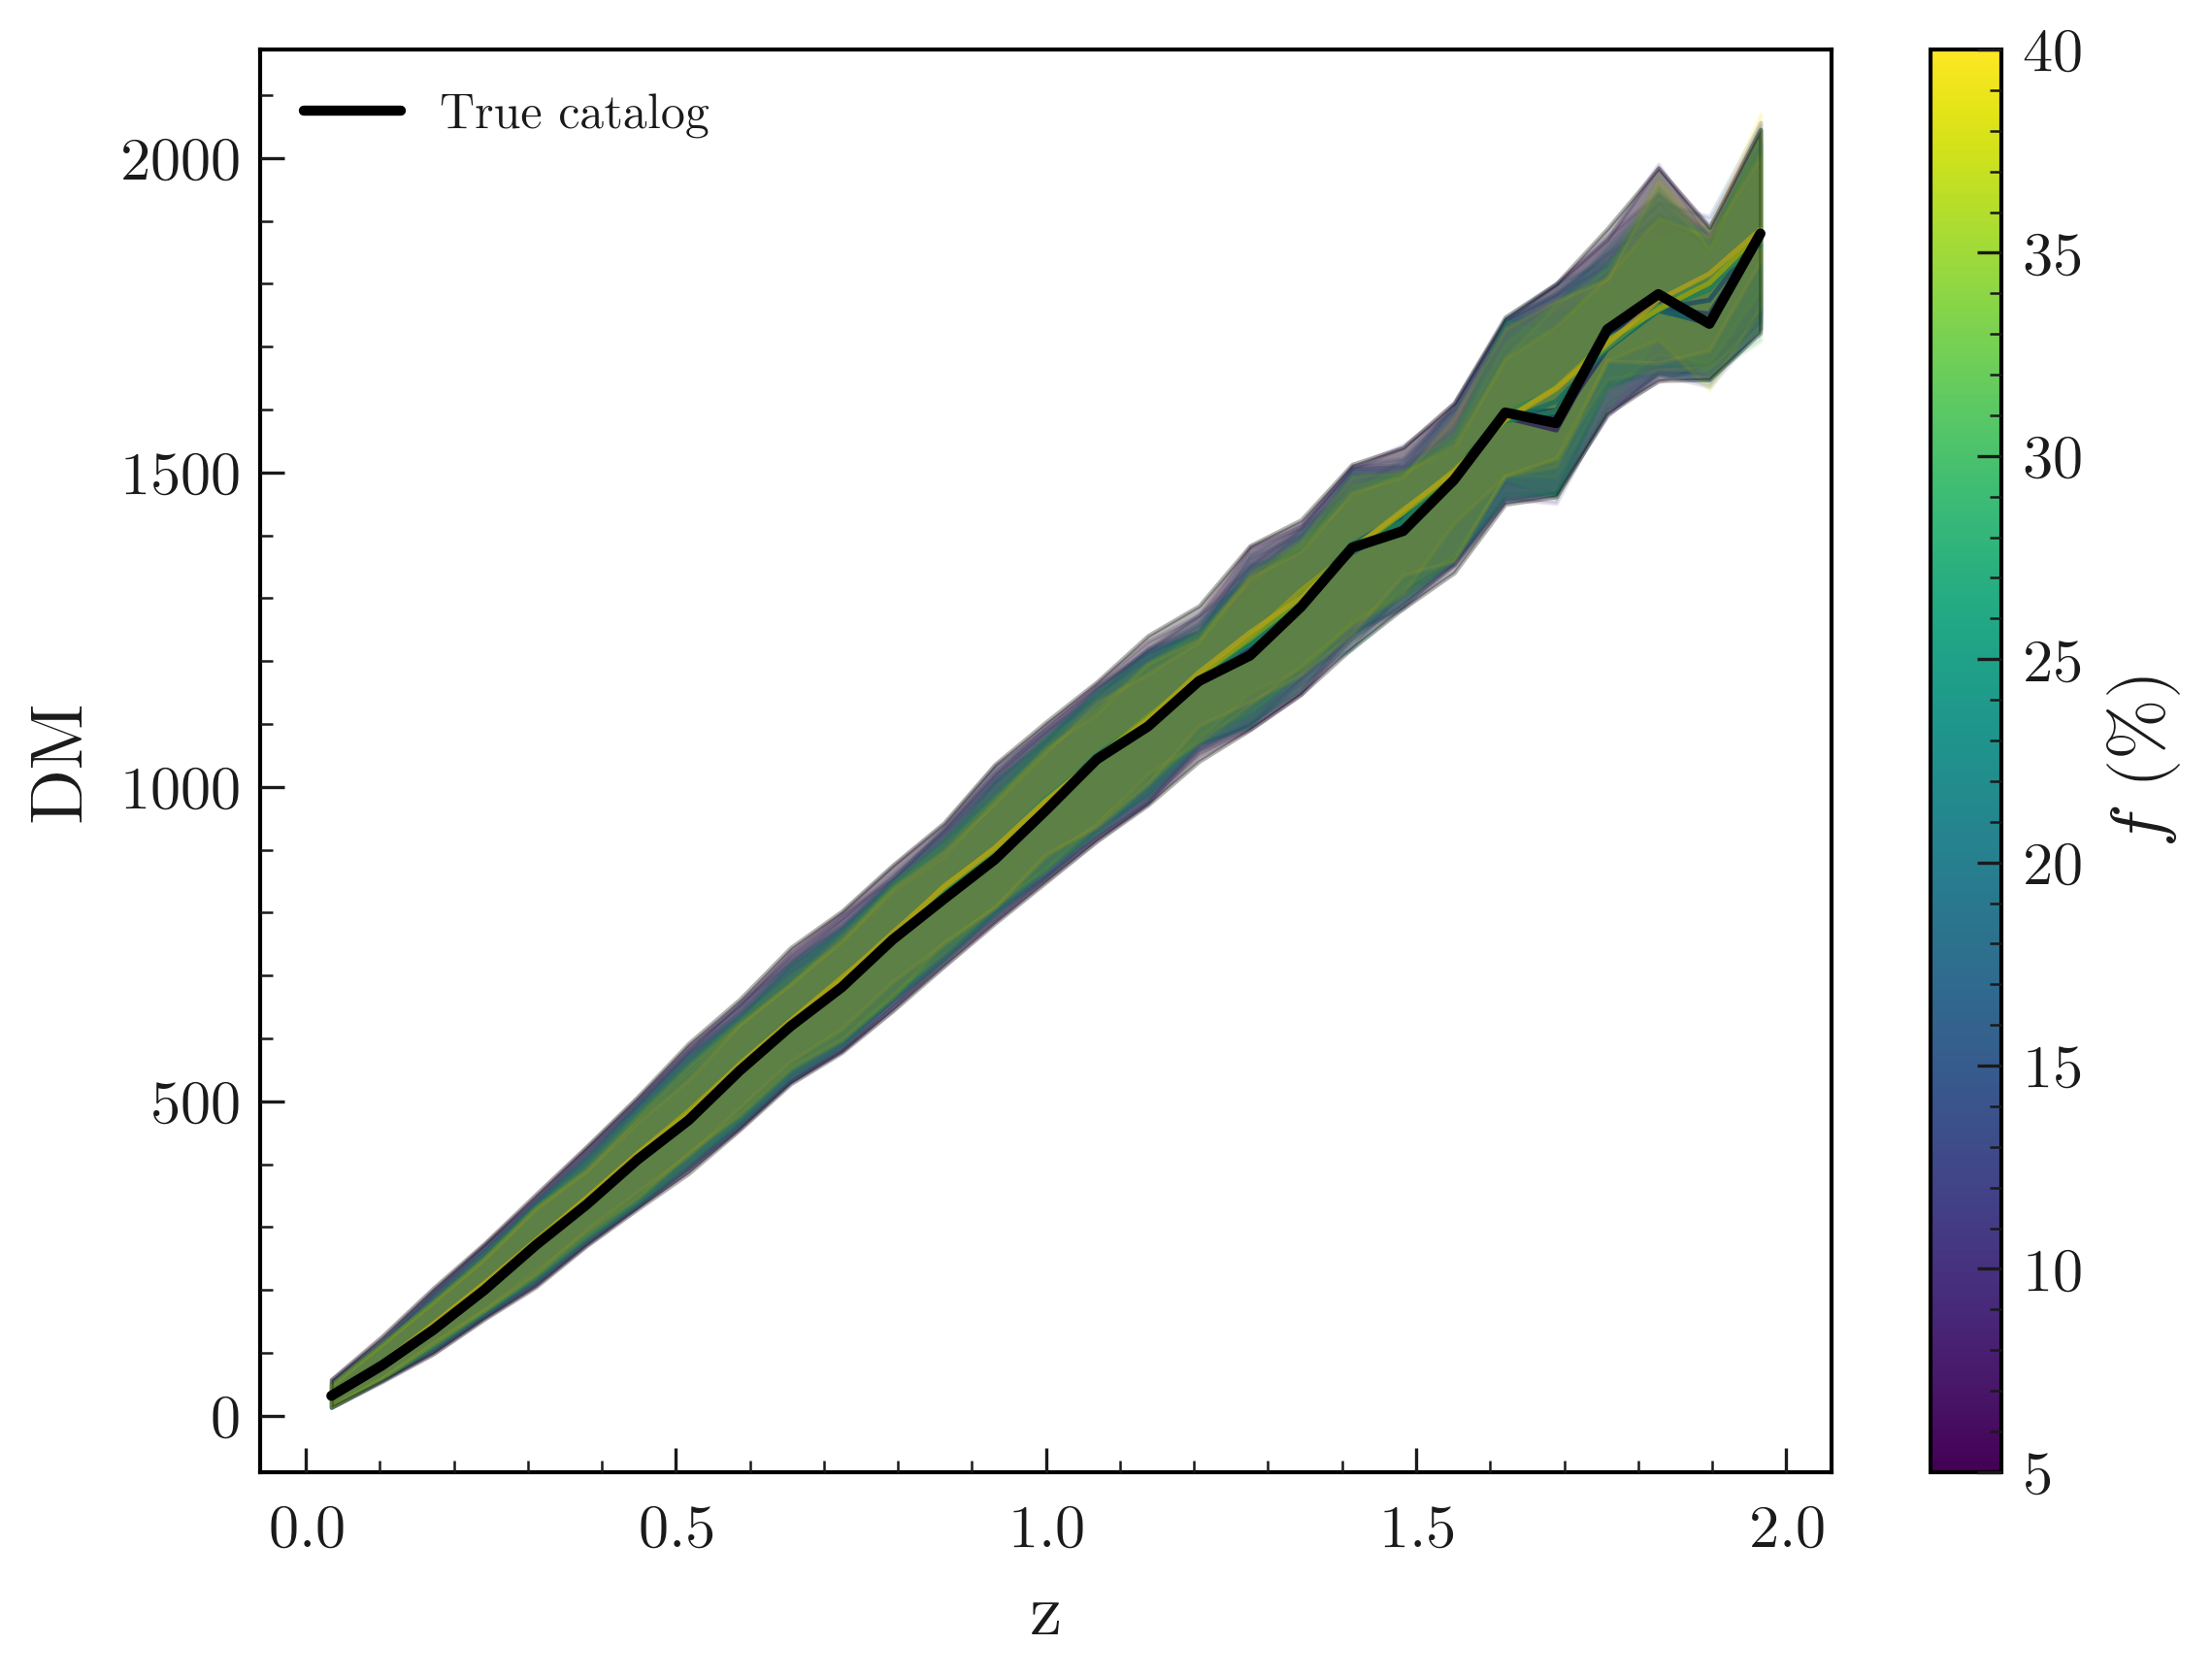
\includegraphics[width=\textwidth]{figs/dm_z_uncertainty_missing_z_random.png}
        \caption{DM-$z$ relation for a random subset of unlocalised hosts.}
    \end{subfigure}
    \hfill
    \begin{subfigure}[t]{0.48\textwidth}
        \centering
        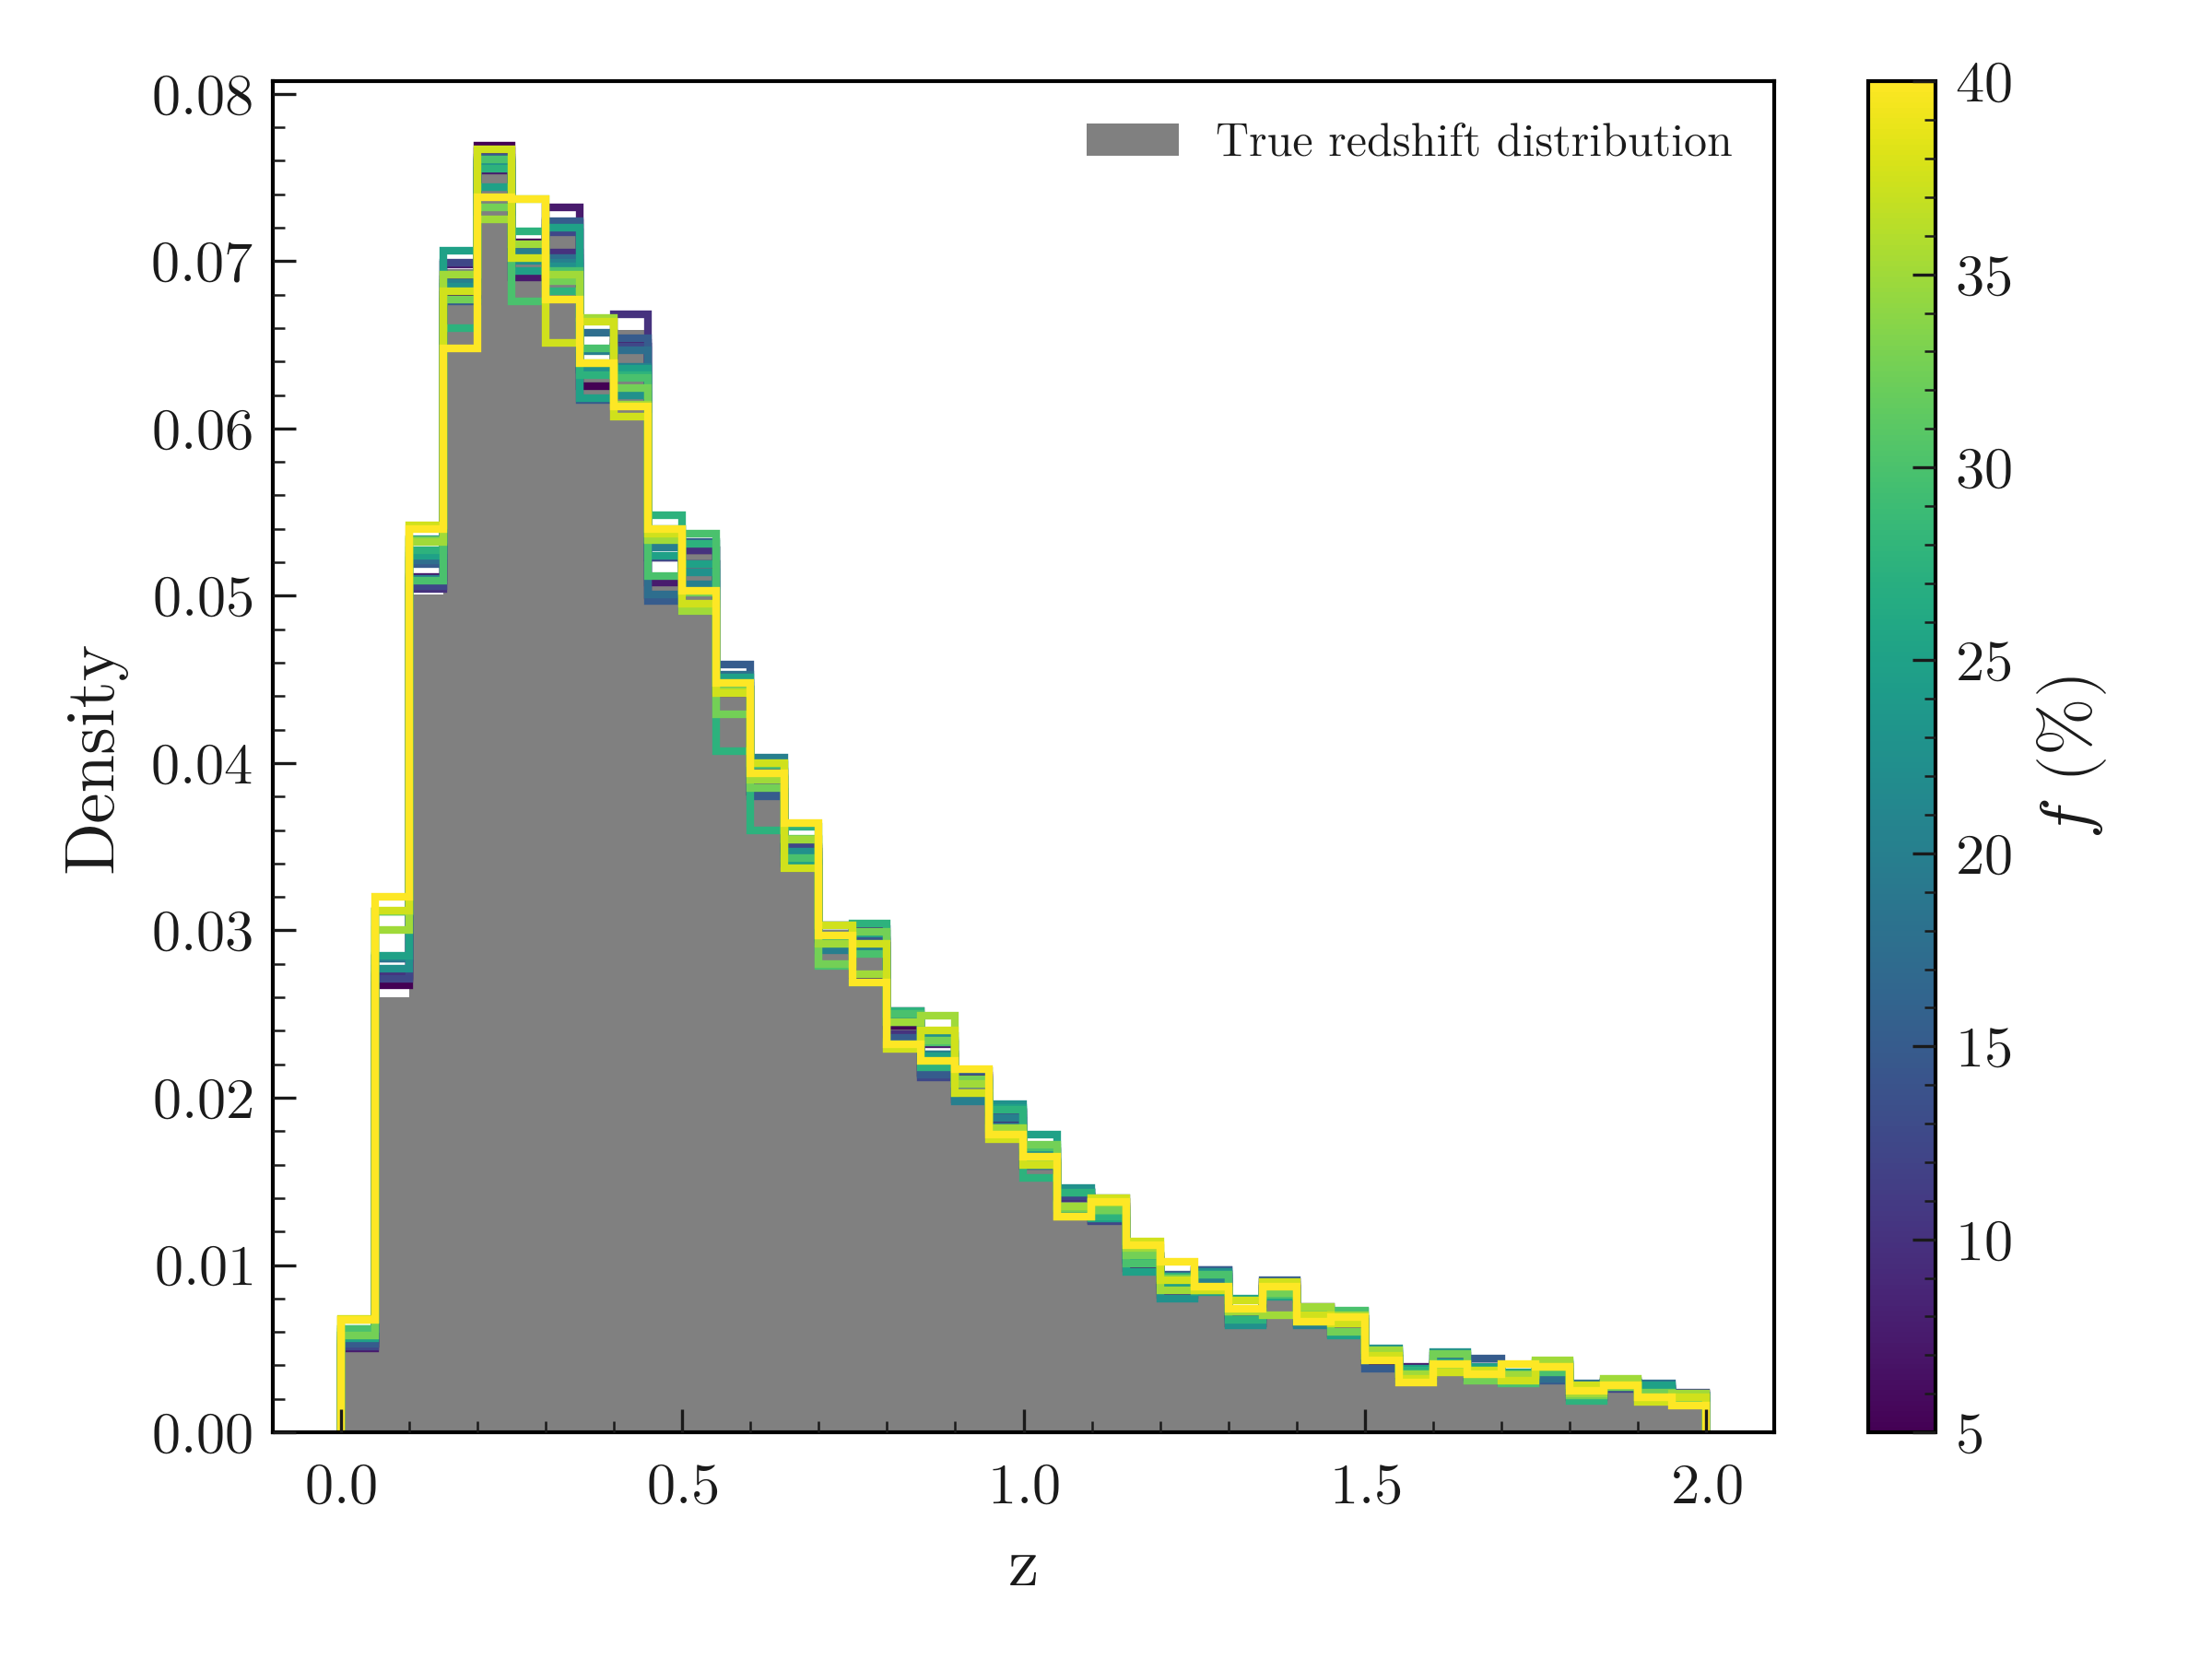
\includegraphics[width=\textwidth]{figs/pdf_uncertainty_missing_z_random.png}
        \caption{PDF of DM for a random subset of unlocalised hosts.}
    \end{subfigure}
    \caption{DM-$z$ relation and PDF for the case of a random subset of unlocalised hosts.}
    \label{res_fig:unloc_random_dmz_pdf}
\end{figure}

The $\chi^2$ value shown in Fig. \ref{res_fig:unloc_random_chisq} fluctuates for different values of $f$ since the process of choosing unlocalised FRBs is random. Nonetheless, the deviation from the true catalog ranges between 1$\sigma$ and 2.5$\sigma$.



\begin{figure}[h!]
    \centering
    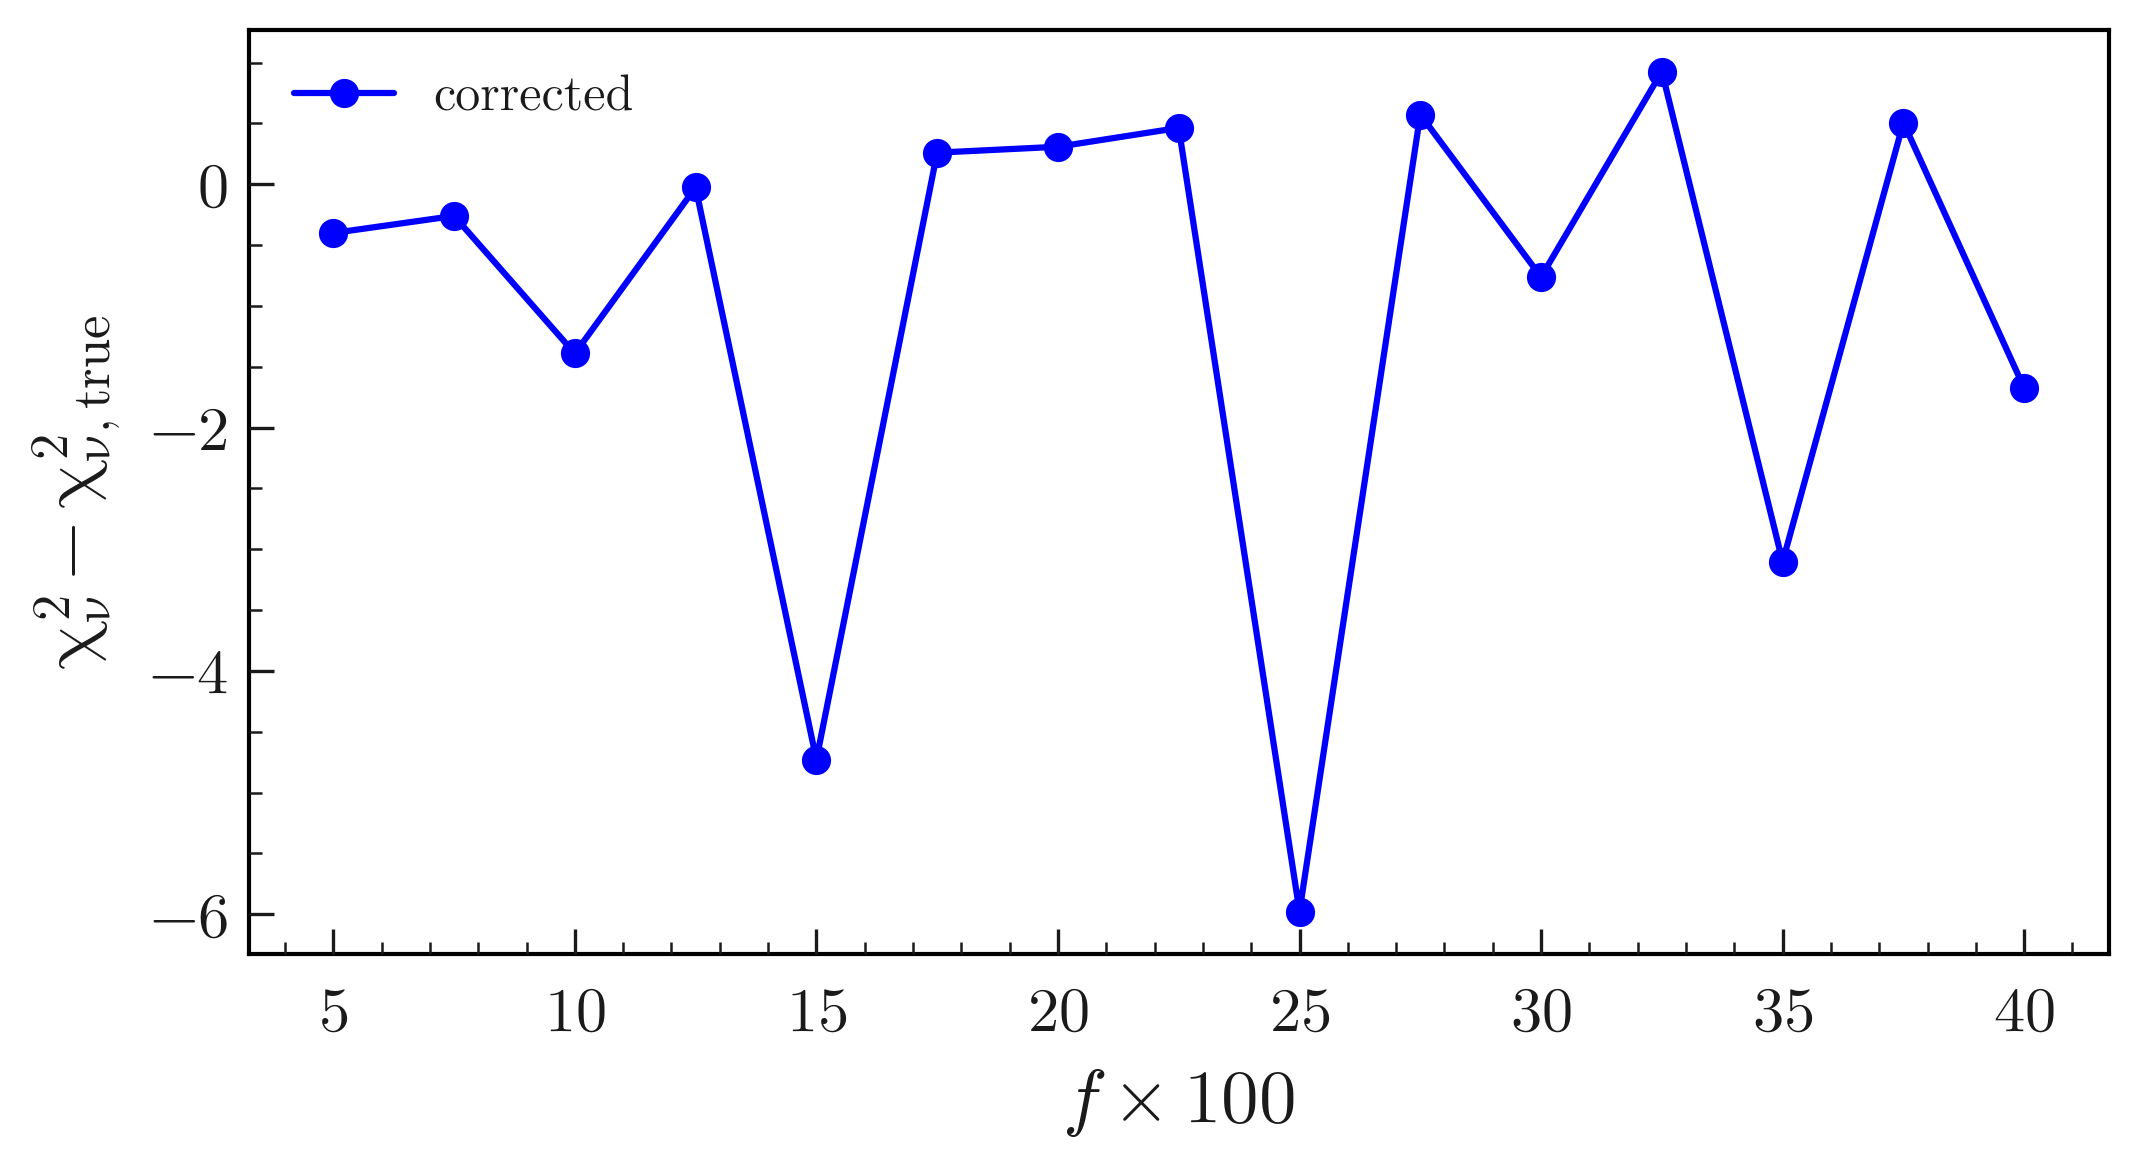
\includegraphics[width=0.6\textwidth]{figs/chi_squared_missing_z_random.png}
    \caption{$\chi^2$ as a function of the fraction of unlocalised hosts for the random subset case.}
    \label{res_fig:unloc_random_chisq}
\end{figure}

% --- High-redshift subset ---
Fig. \ref{res_fig:unloc_highz_dmz_pdf} shows the variation of the DM-$z$ relation and the PDF for a fraction of unlocalised hosts with high redshifts. The left-hand side of the figure shows the mean of the DM-$z$ relation is consistent with the fiducial catalog, but the variance is underestimated. This is due to mapping a measured DM in the contaminated catalog to the corresponding redshift according to the fiducial mean DM-$z$ relation. This is reflected on the right-hand side plot with the shape of the PDF changing for large values of DM since this corresponds to unlocalised sources at high $z$.

\begin{figure}[h!]
    \centering
    \begin{subfigure}[t]{0.48\textwidth}
        \centering
        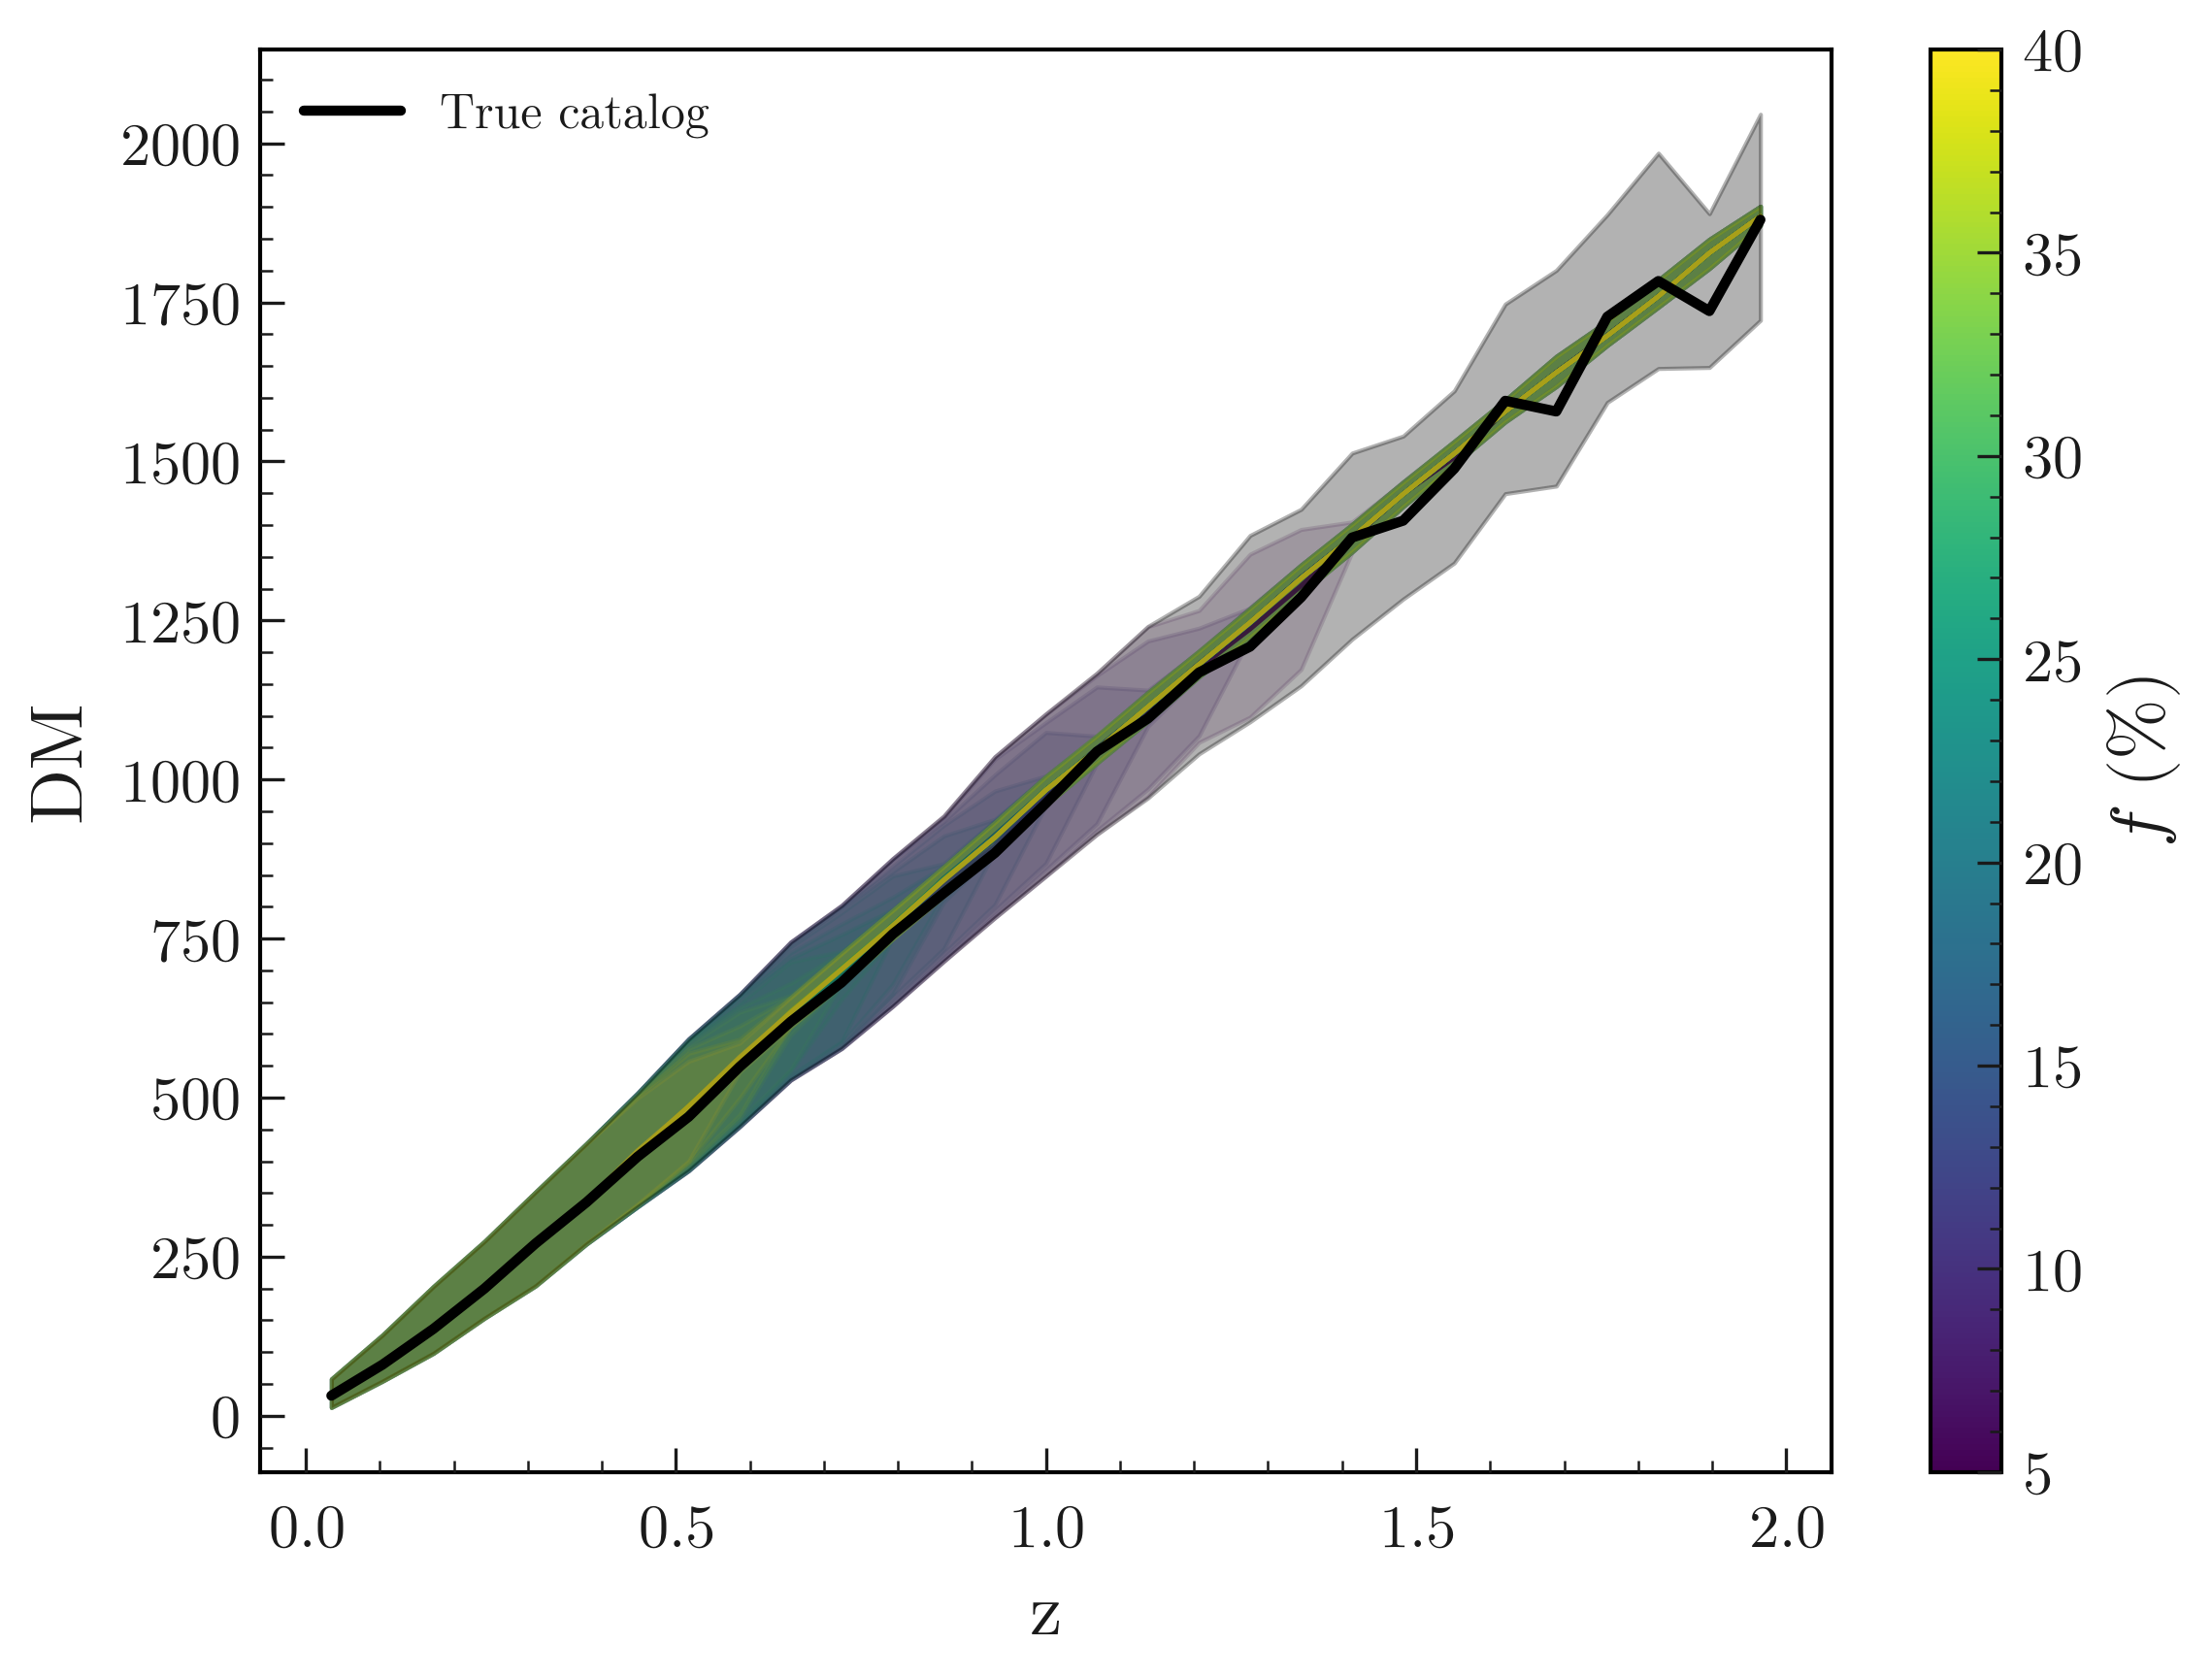
\includegraphics[width=\textwidth]{figs/dm_z_uncertainty_missing_z_high_z.png}
        \caption{DM-$z$ relation when high-$z$ FRBs are unlocalised.}
    \end{subfigure}
    \hfill
    \begin{subfigure}[t]{0.48\textwidth}
        \centering
        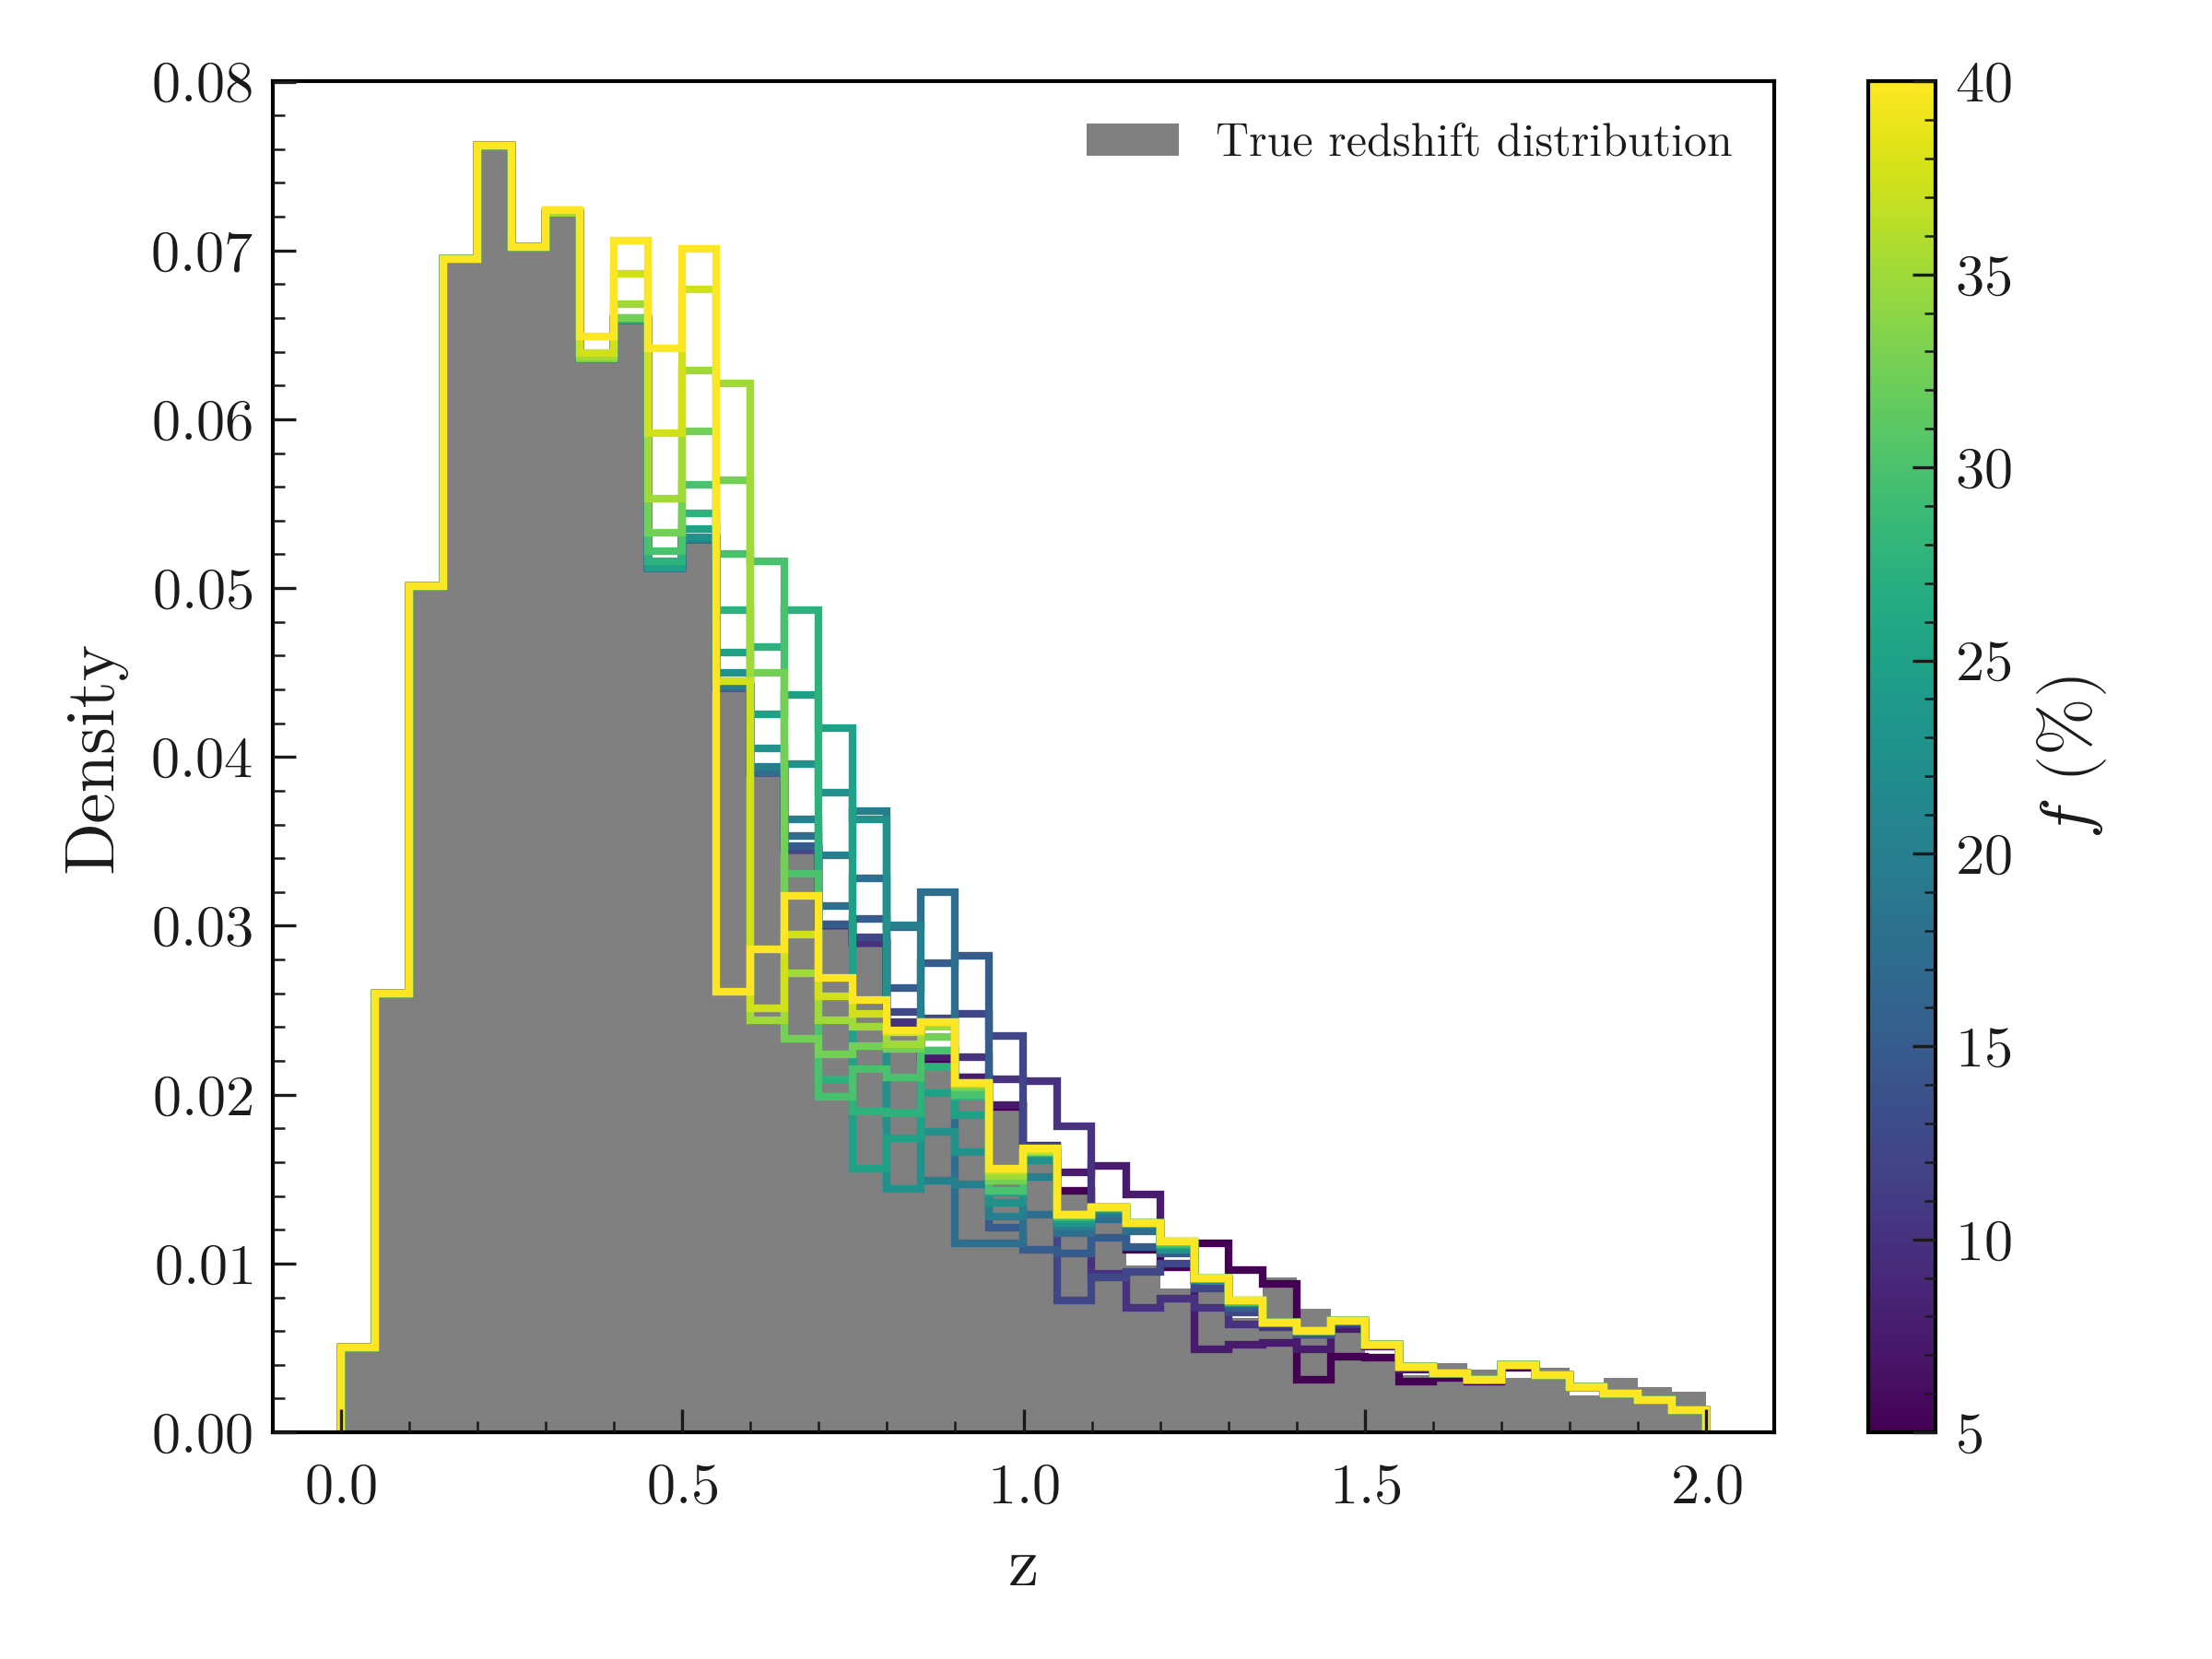
\includegraphics[width=\textwidth]{figs/pdf_uncertainty_missing_z_high_z.png}
        \caption{PDF of DM when high-$z$ FRBs are unlocalised.}
    \end{subfigure}
    \caption{DM-$z$ relation and PDF for the case where high-redshift FRBs are unlocalised.}
    \label{res_fig:unloc_highz_dmz_pdf}
\end{figure}

Fig. \ref{res_fig:unloc_highz_chisq} shows a significant deviation from the true value of $\chi^2$. The deviation reaches 5$\sigma$ for larger fraction of missing redshifts, but the deviation is only 1$\sigma$ for $f \approx 25\%$. The deviation is larger compared to the case of randomly unlocalised hosts since sources at high redshifts have a stronger signal since DM is an integrated effect along the line of sight and FRBs from higher redshift correspond to larger DM values.



\begin{figure}[h!]
    \centering
    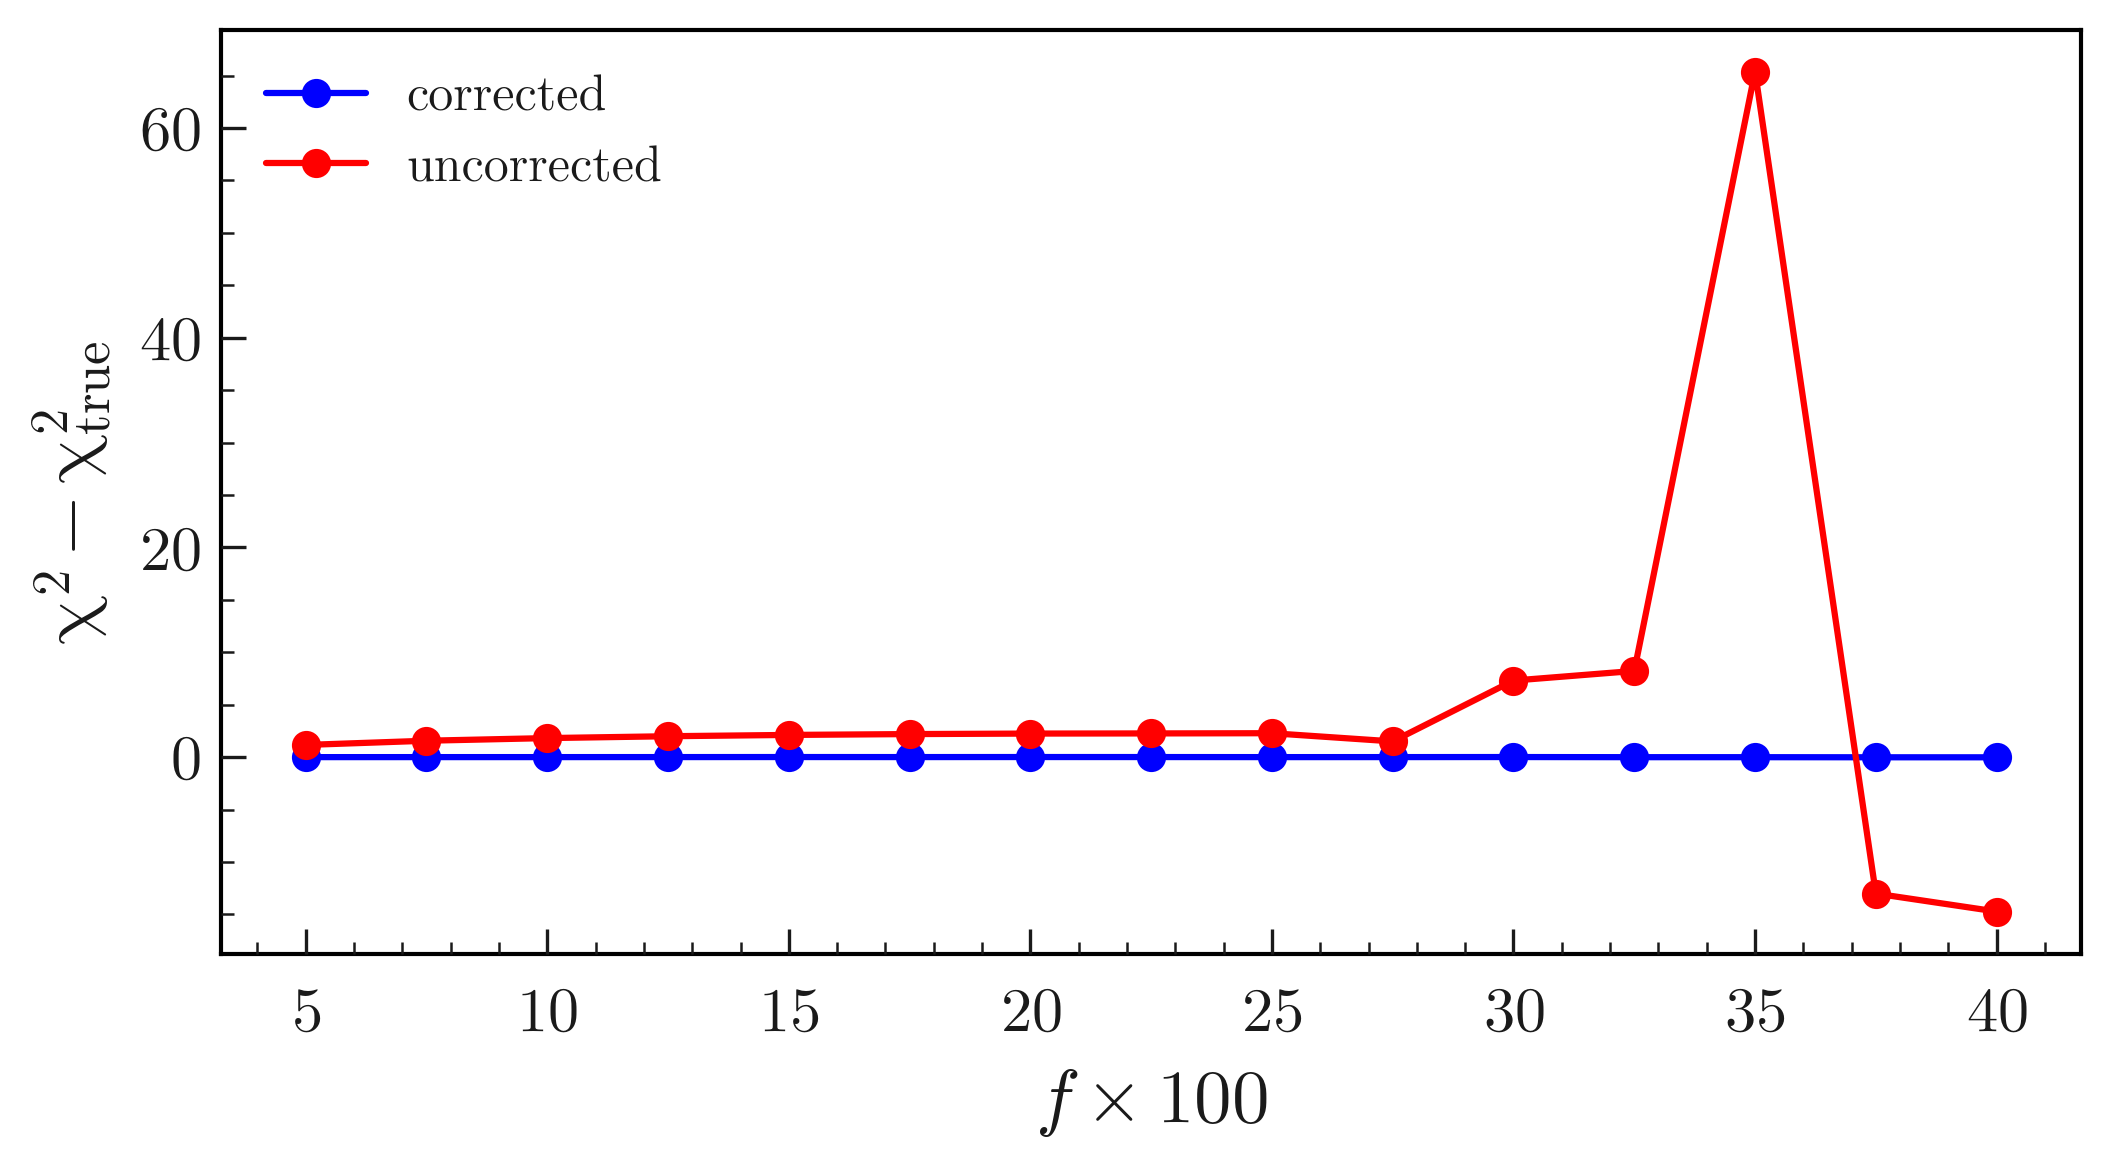
\includegraphics[width=0.6\textwidth]{figs/chi_squared_missing_z_high_z.png}
    \caption{$\chi^2$ as a function of the fraction of unlocalised hosts for the high-redshift subset case.}
    \label{res_fig:unloc_highz_chisq}
\end{figure}

% --- Low-redshift subset ---
The left-hand side of Fig. \ref{res_fig:unloc_lowz_dmz_pdf} shows the variation in the DM-$z$ relation when a fraction of low redshift FRBs has unlocalised hosts. The left-hand side shows a slight deviation of the variance from the variance of the fiducial catalog at low redshift while the mean of the contaminated catalog is consistent with that of the fiducial catalog for the entirety of the redshift range and for varying fraction of the unlocalised hosts. The PDF on the other hand shows a deviation of the peak with larger values of $f$. In addition the shape of the PDF changes at low values of $z$. However, the width of the PDF does not change, reflecting the unchanging variance from the left-hand side plot.

\begin{figure}[h!]
    \centering
    \begin{subfigure}[t]{0.48\textwidth}
        \centering
        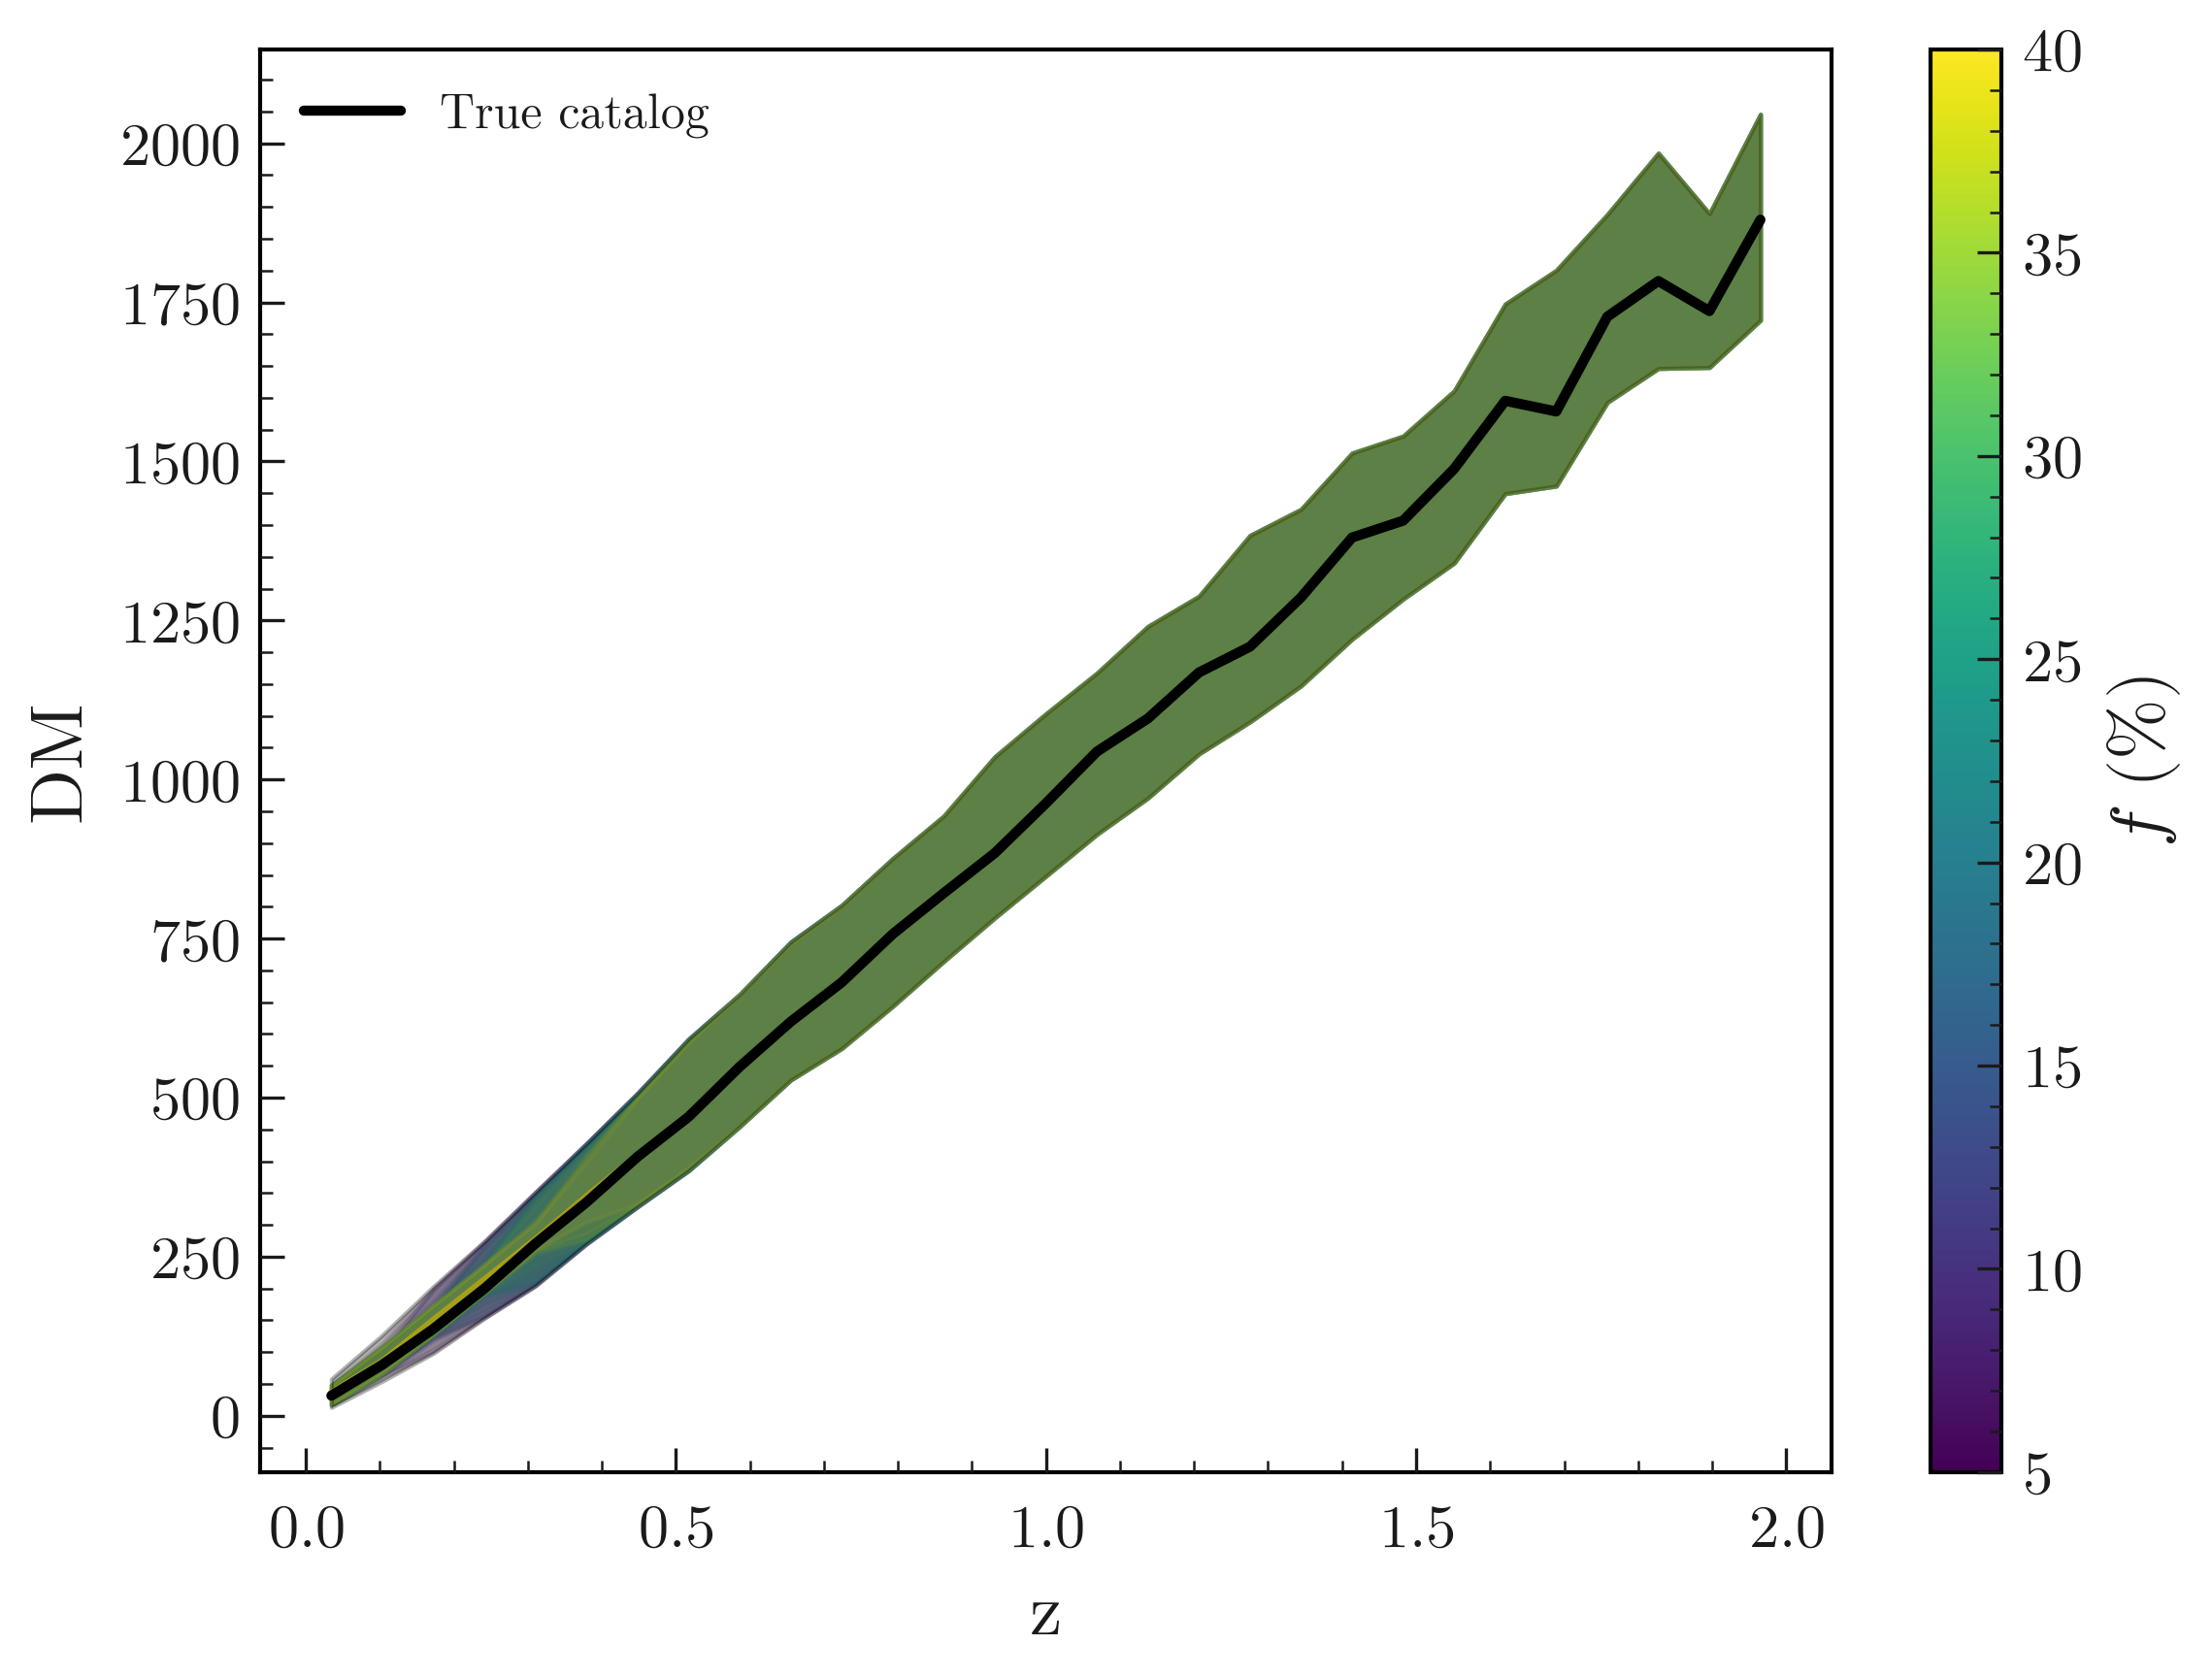
\includegraphics[width=\textwidth]{figs/dm_z_uncertainty_missing_z_low_z.png}
        \caption{DM-$z$ relation when low-$z$ FRBs are unlocalised.}
    \end{subfigure}
    \hfill
    \begin{subfigure}[t]{0.48\textwidth}
        \centering
        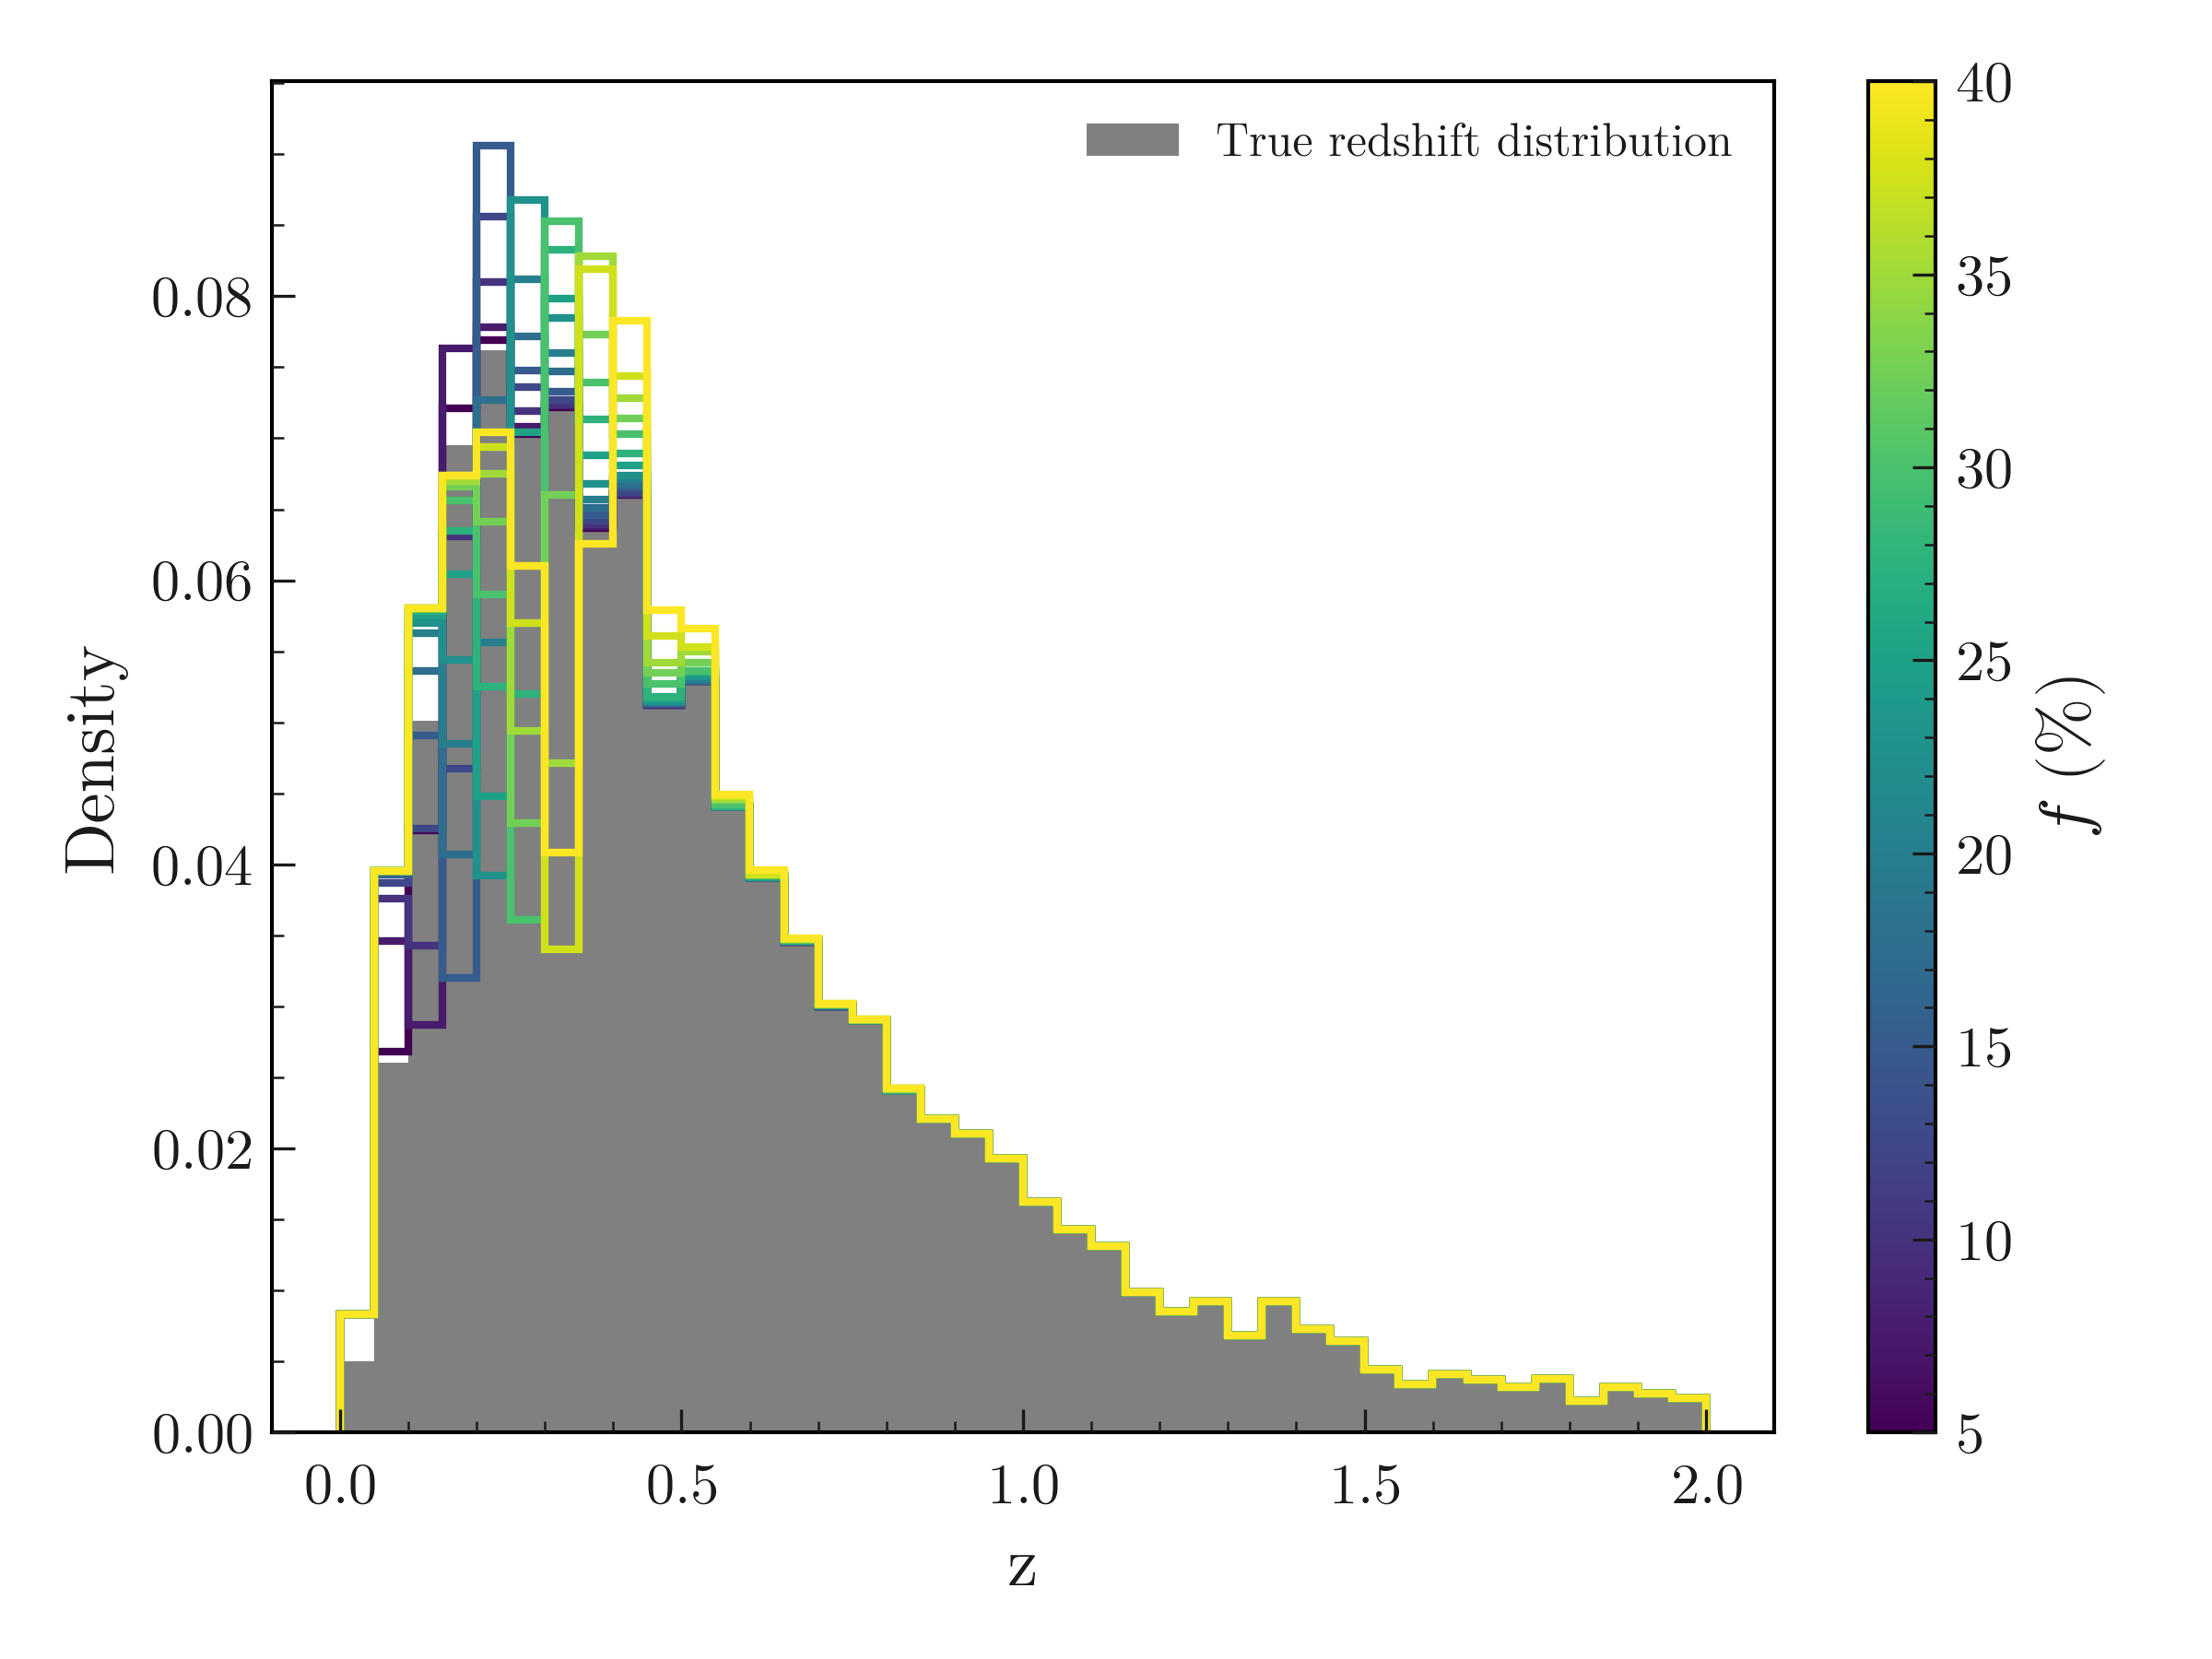
\includegraphics[width=\textwidth]{figs/pdf_uncertainty_missing_z_low_z.png}
        \caption{PDF of DM when low-$z$ FRBs are unlocalised.}
    \end{subfigure}
    \caption{DM-$z$ relation and PDF for the case where low-redshift FRBs are unlocalised.}
    \label{res_fig:unloc_lowz_dmz_pdf}
\end{figure}

The variation of the $\chi^2$ in Fig. \ref{res_fig:unloc_lowz_chisq} is consistent with the variation observed from the left-hand side plot of Fig. \ref{res_fig:unloc_lowz_dmz_pdf} where the deviation due to unlocalised hosts at low redshift does not exceed $1\sigma$ for the range of $f$ considered in this study. This can be corroborated by noticing that low redshift sources have a lower signal since the physical distance that the pulse covers is small as compared to high redshift sources.

\begin{figure}[h!]
    \centering
    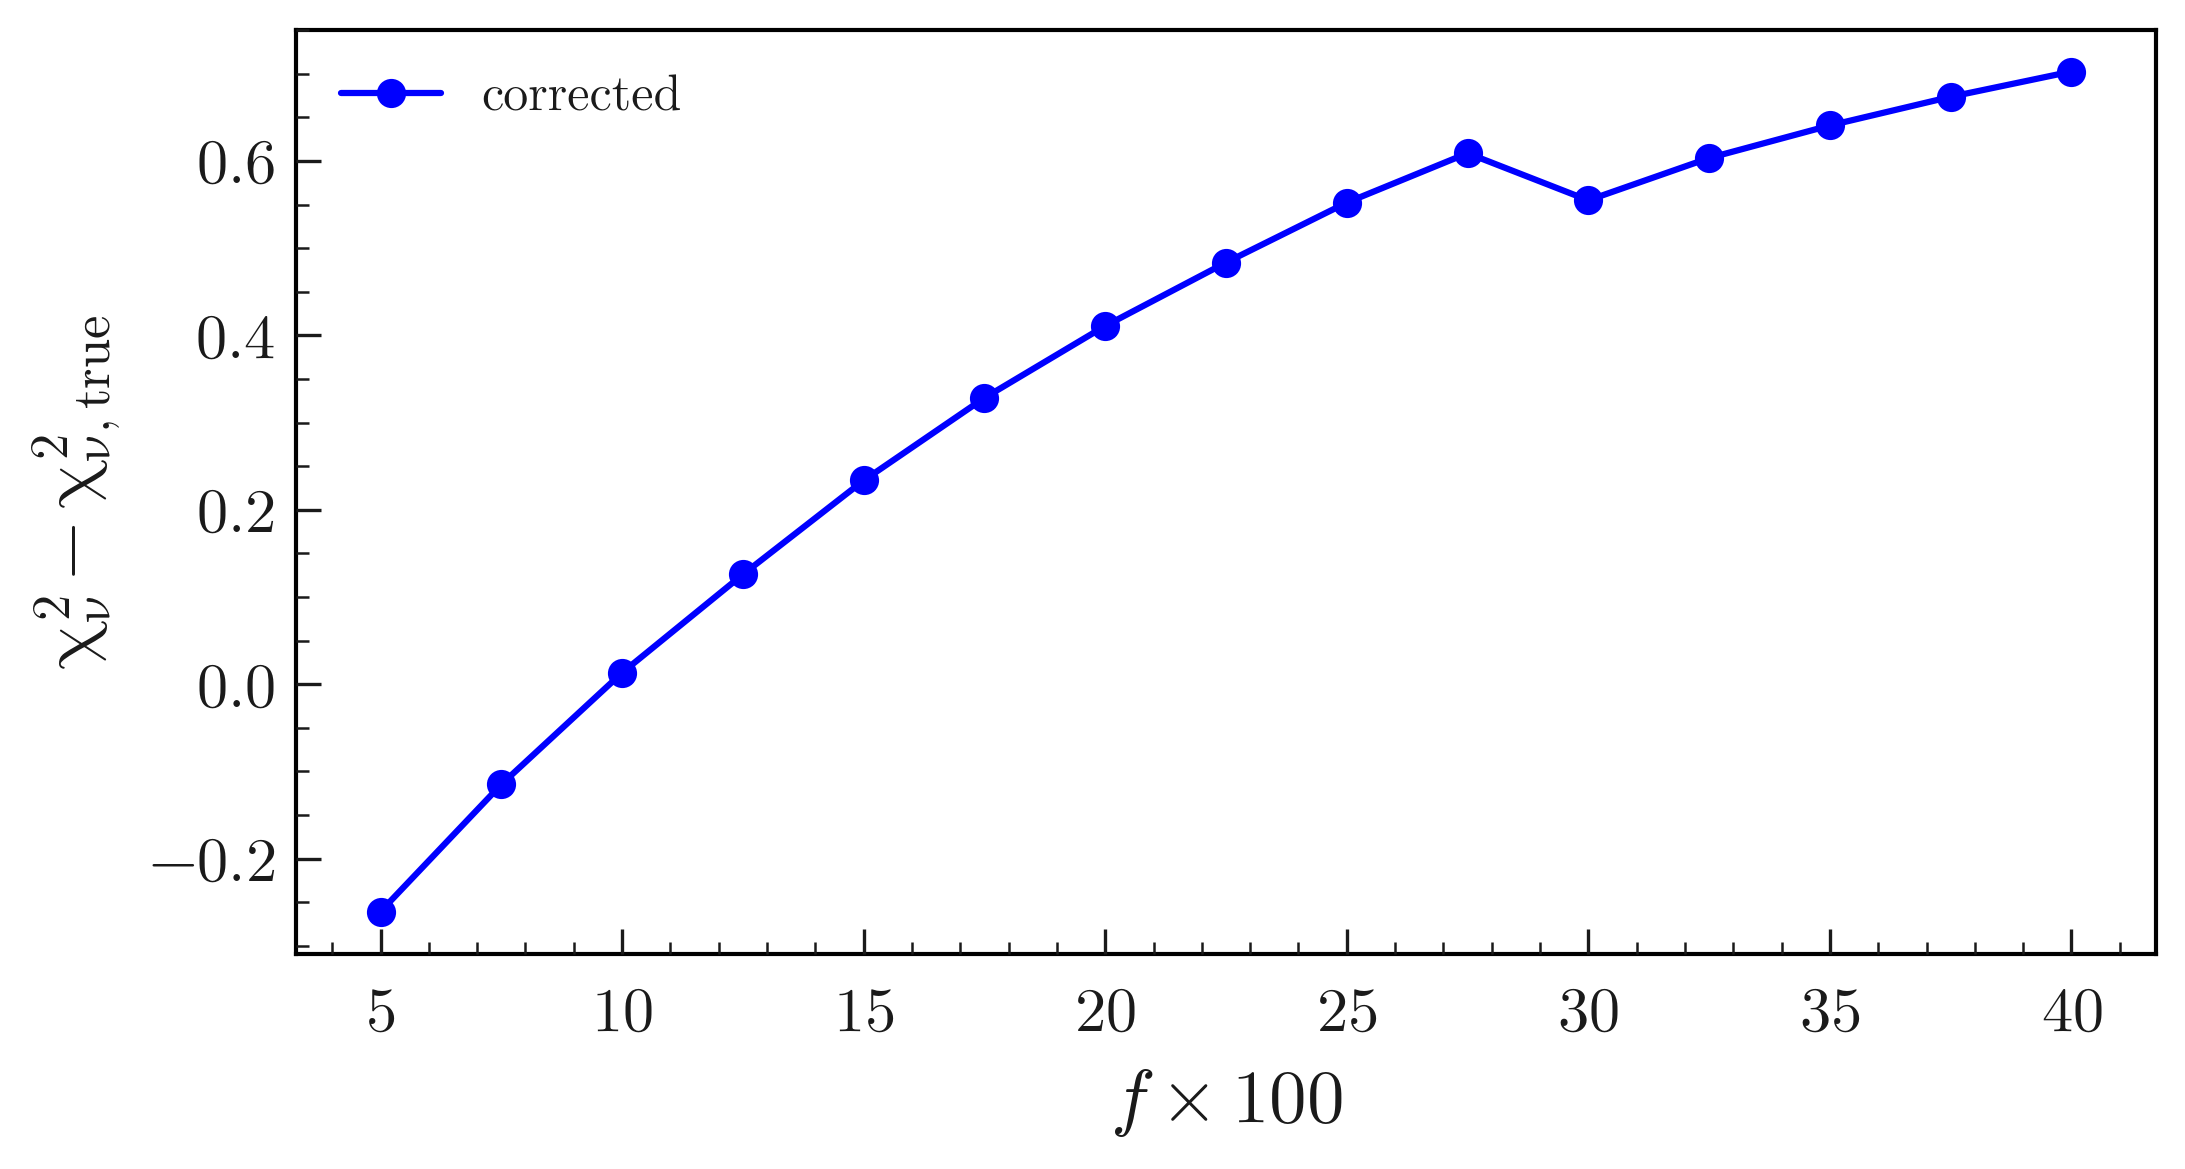
\includegraphics[width=0.6\textwidth]{figs/chi_squared_missing_z_low_z.png}
    \caption{$\chi^2$ as a function of the fraction of unlocalised hosts for the low-redshift subset case.}
    \label{res_fig:unloc_lowz_chisq}
\end{figure}

In total, using unlocalised hosts at high redshifts yields the largest deviation in the DM-$z$ relation while random unlocalised hosts also yields a significant deviation but less than the case for high redshifts. In practice, this can inform a strategy for optical follow-up observation where high redshift sources are more 'rewarding' to observe as compared to low redshift sources. Nonetheless, the redshifts of the sources are not known a priori, however, it can be estimated from the measured value of DM whether the source is at higher or low redshift where larger values of DM indicate that the FRB is more probable to originate at high redshifts.


\section{Results from Simulation Based Inference}
In this section, I present the results from SBI for randomly unlocalised FRBs and redshift uncertainty. For the redshift uncertainty I choose a value of $\eta = 0.25$ to contaminate the catalog. For randomly unlocalised hosts, I choose $f = 0.25$. Both numbers are chosen to be intermediate values of the considered range of uncertainty parameters.

Fig. \ref{res_fig:sbi_missing_z} shows the parameter constraints using SBI for the case of randomly unlocalised hosts. The posterior is trained for 4 rounds with a total of 6000 simulations. I used MAF architecture with 10 transformations and 40 hidden features with 2 blocks for each individual map. The TARP test was not performed for this case since the resulting posterior is not constraining of the model parameters where for each contour plots the resulting posterior is prior dominated except that of $\Omega_\mathrm{b} - h$ where the direction of the degeneracy is recovered. Nonetheless, it is possible to see that the obtained constraints on the rest of the parameters are biased with respect to the fiducial model parameters. This is directly related to what can be observed in the left-hand side of Fig. \ref{res_fig:unloc_random_dmz_pdf} where the variance of the DM-$z$ relation is different from the fiducial, and the bias propagates to the corresponding parameters that control the variance, in particular $\sigma_8$ and $\log_{10} M_\mathrm{c}$.

\begin{figure}[h!]
    \centering
    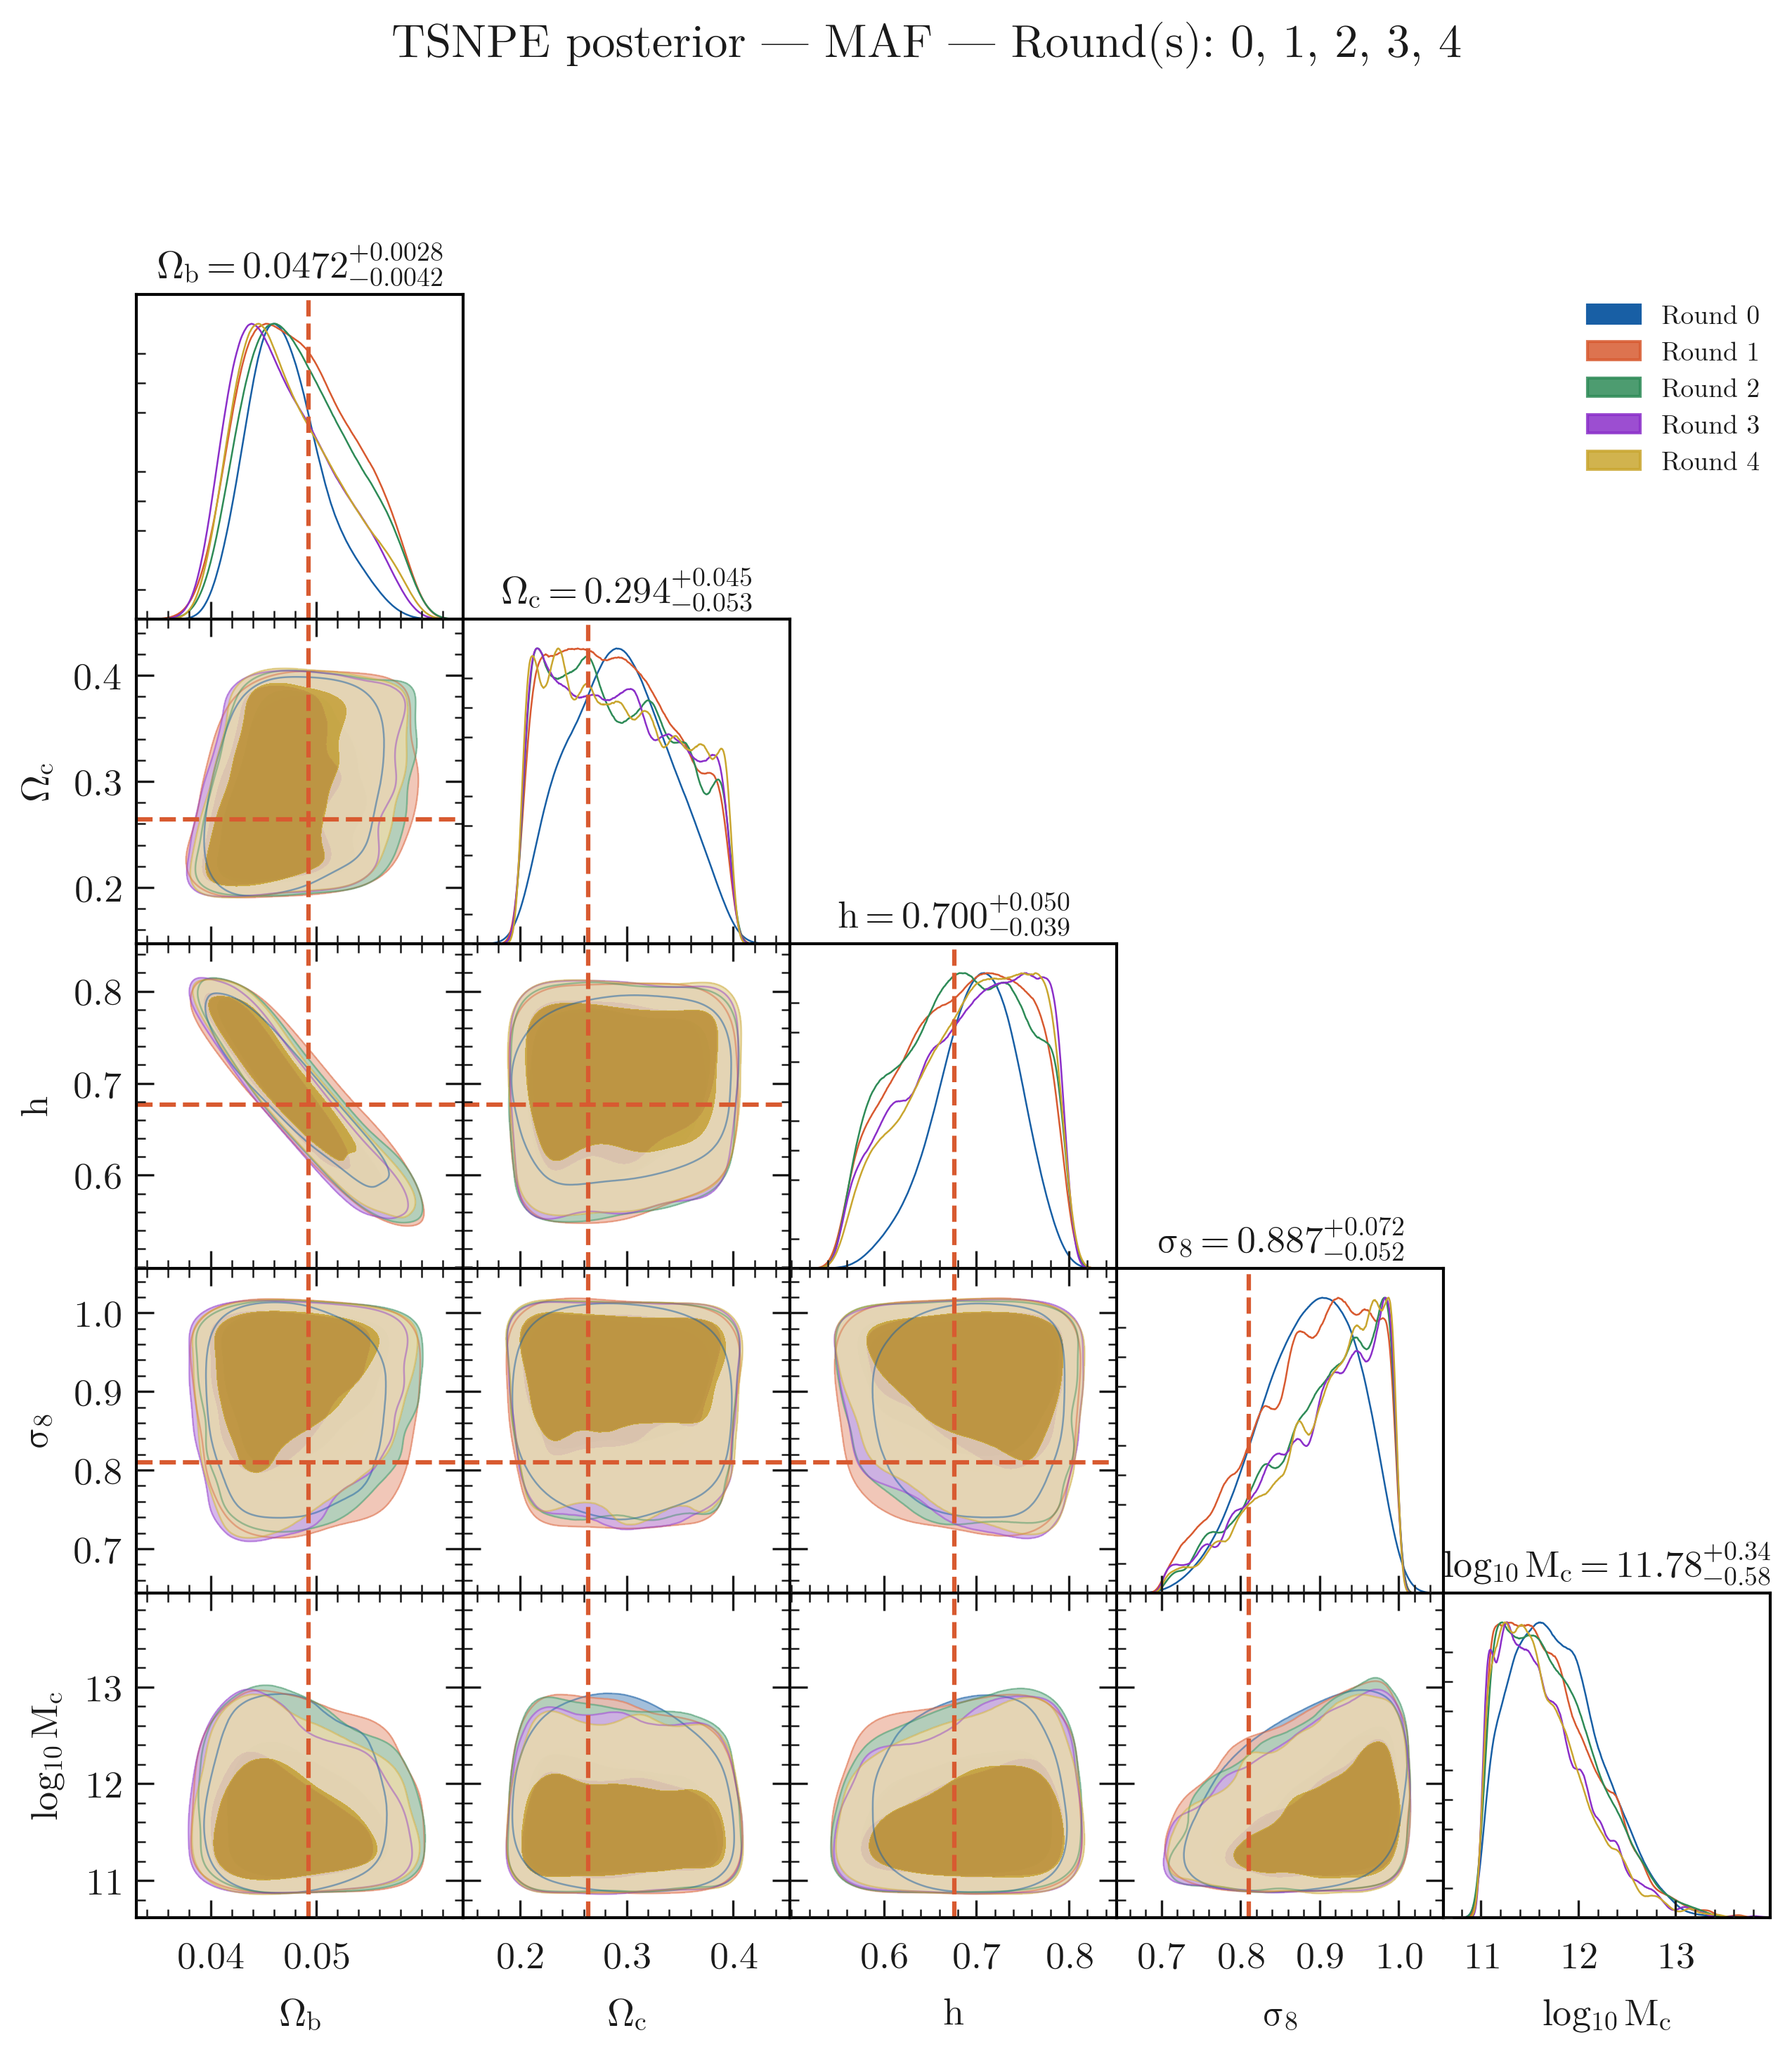
\includegraphics[width=0.9\textwidth]{figs/20260420_005327_missing_z_r00_r01_r02_r03_r04.png}
    \caption{Posterior distributions from SBI for the missing redshift scenario.}
    \label{res_fig:sbi_missing_z}
\end{figure}


Similarly, Fig. \ref{res_fig:sbi_z_uncertainty} shows parameter constraints using SBI using a catalog contaminated with redshift uncertainty. In this case, I use MDN with 30 hidden features and 5 components. By looking at the contours of $\Omega_\mathrm{b} - h$, the degeneracy between these two parameters is recovered since the redshift uncertainty with $\eta = 0.25$ does not affect the mean DM-$z$ relation as per Fig. \ref{res_fig:redshift_dmz_pdf}. Meanwhile, since the variance is different as compared to fiducial catalog, the constraints in the $\sigma_8-\log_{10} M_\mathrm{c}$ are biased with respect to the fiducial parameters. In addition, there is a positive degeneracy between $\sigma_8$ and $\log_{10} M_\mathrm{c}$ since both parameters control the amplitude of the gas power spectrum and therefore the overall amplitude of the variance.


\begin{figure}[h!]
    \centering
    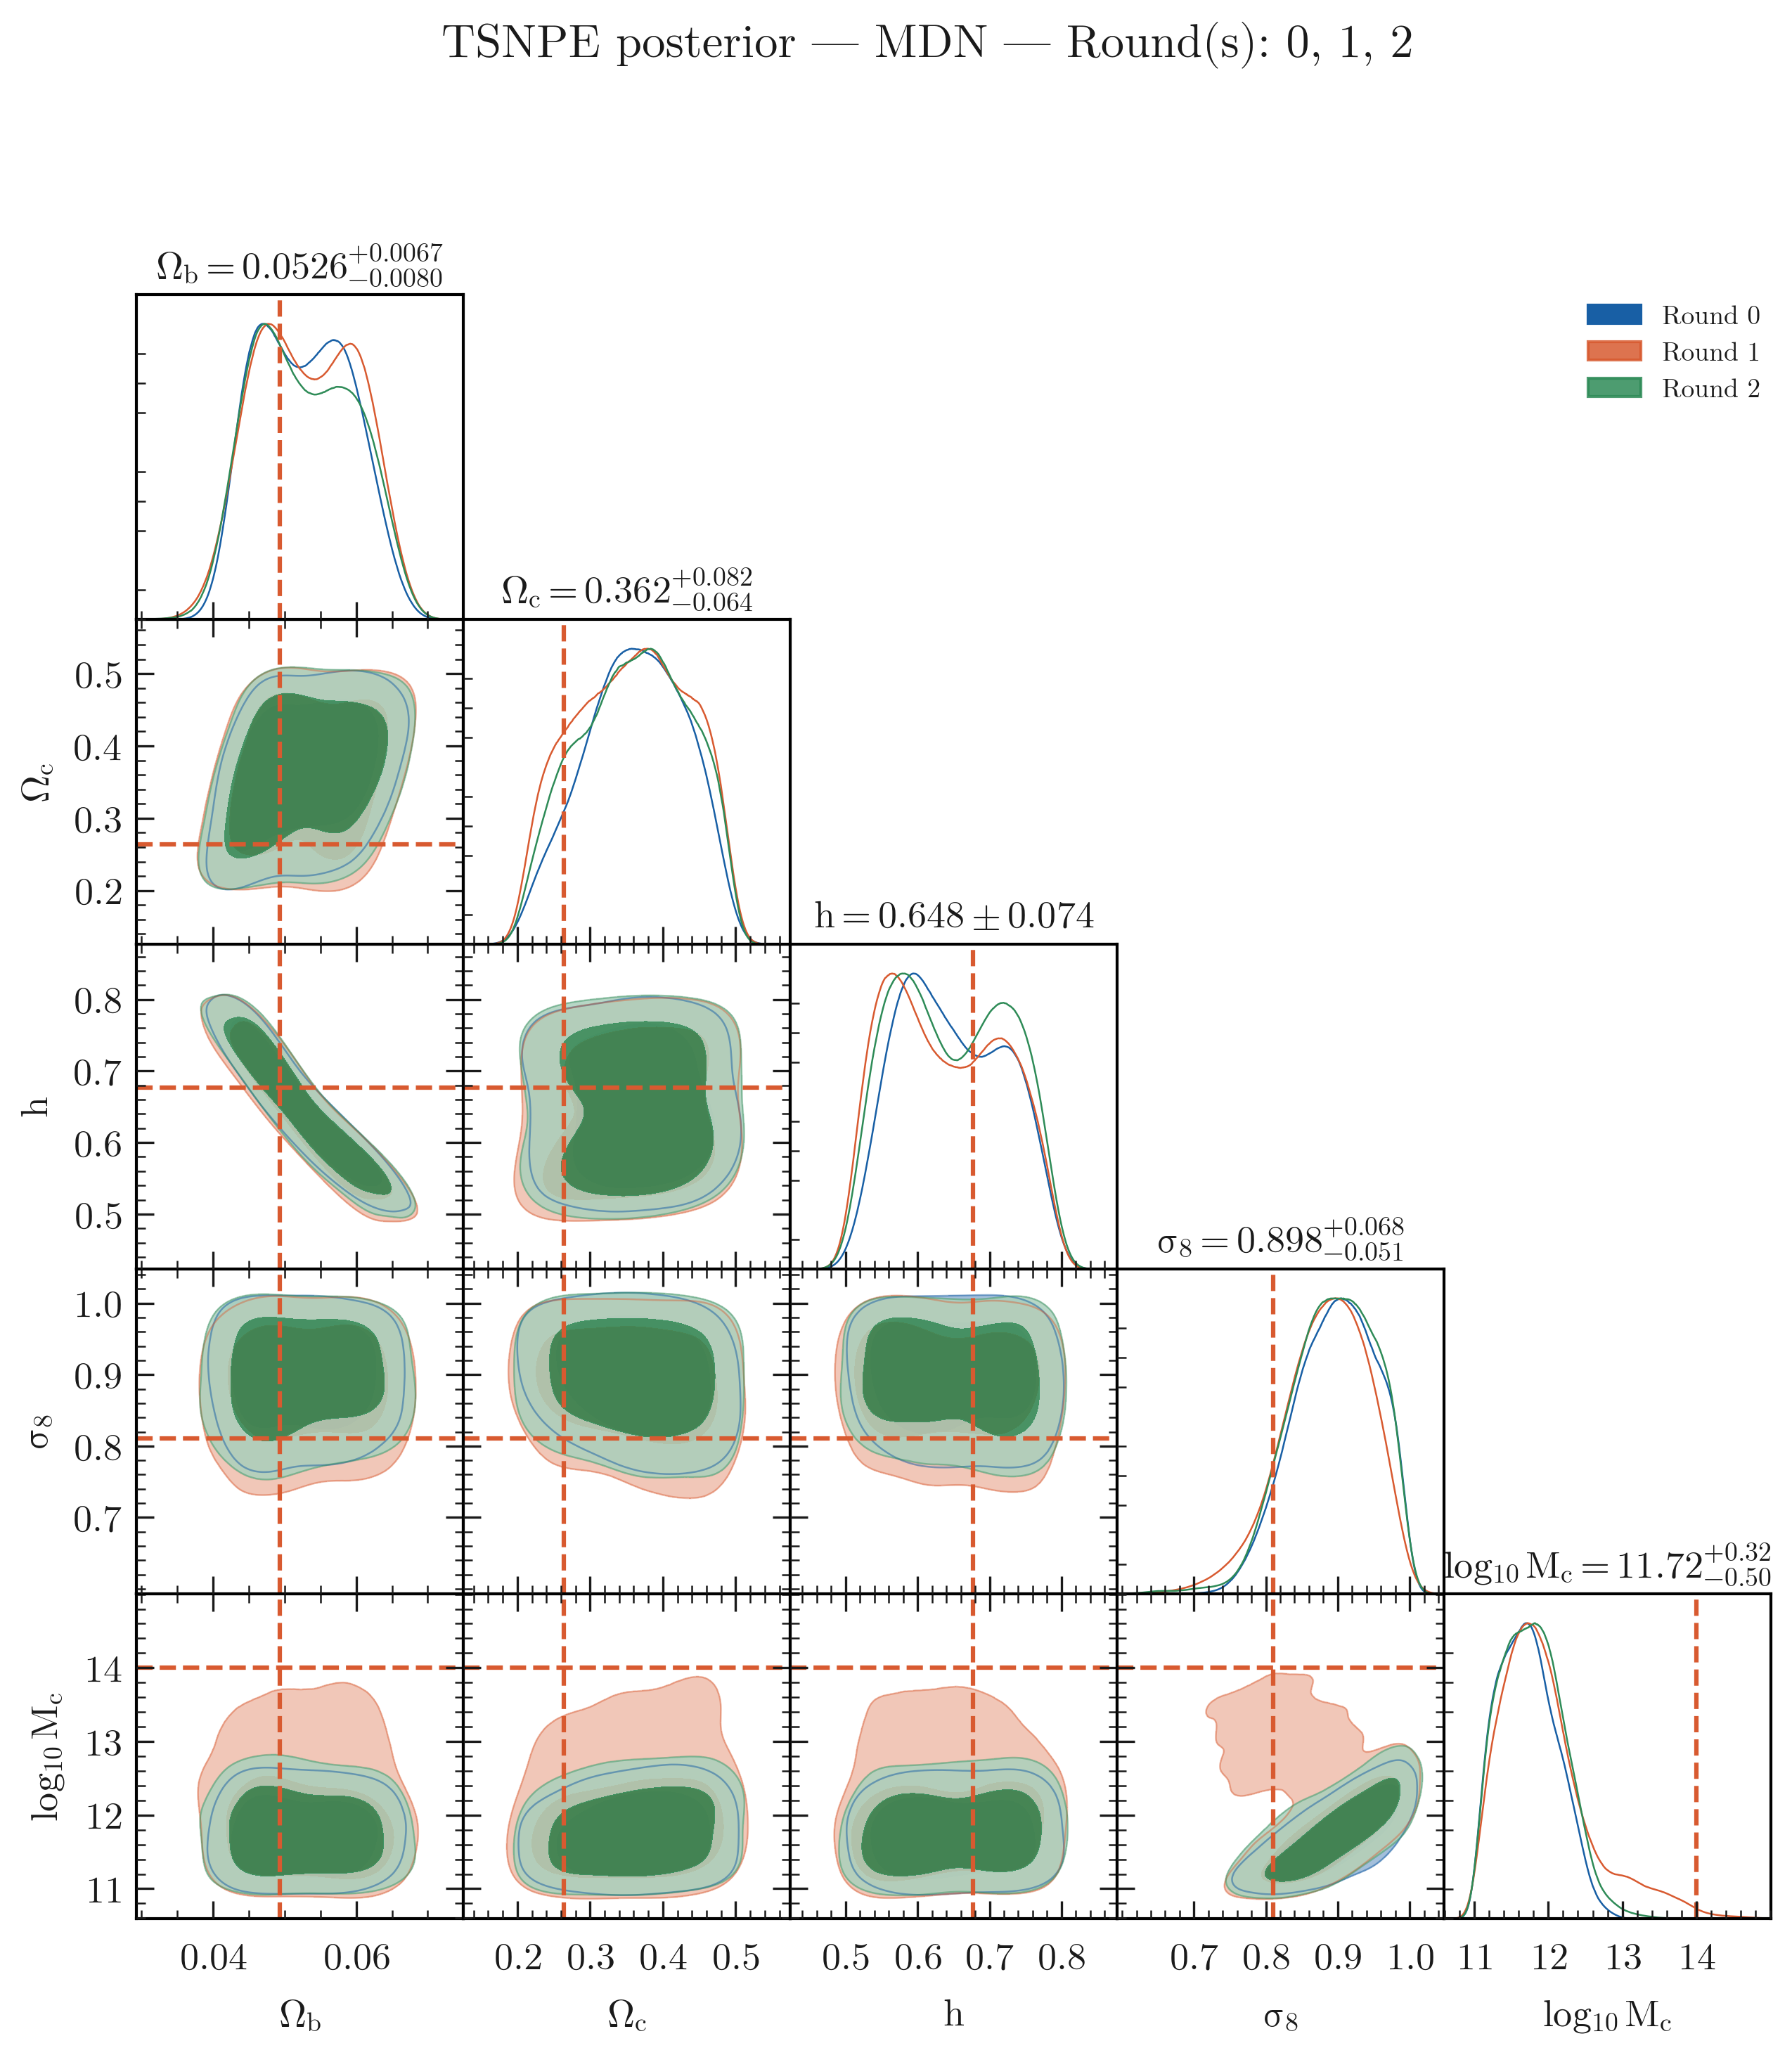
\includegraphics[width=0.9\textwidth]{figs/20260420_200557_z_uncertainty_r00_r01_r02.png}
    \caption{Posterior distributions from SBI for the redshift uncertainty scenario.}
    \label{res_fig:sbi_z_uncertainty}
\end{figure}



To understand the reasons behind prior domination and unconstrained $\Omega_\mathrm{c}$, I ran the After many tests, the optimal architecture to be used in this thesis turned out to be 10 transformations, 50 hidden features, and 2 blocks for each individual map. The paraemter constraints are shown in Fig. \ref{res_fig:sbi_fiducial}. Upon performing the TARP test, the inferred posterior is slightly overconfident as compared to the true parameter posterior as can be seen from Fig. \ref{res_fig:sbi_tarp}, but these constraints can be used to improve certain aspects of the inference pipeline in the following way. The parameter degeneracies are recovered both in $\Omega_\mathrm{b} - h$ and $\sigma_8-\log_{10} M_\mathrm{c}$. However, the constraints on $\Omega_\mathrm{c}$ are prior dominated. The reason can be traced back to the choice of summary statistic where the score compression is only sensitive to the mean which scales with the product $\Omega_\mathrm{b} h$ and the scale-independent variance which scales with the amplitude of the power spectrum, with the amplitude of the power spectrum. In the appendix, it is possible to see the variation of power spectrum amplitude with both $\log_{10} M_\mathrm{c}$.


\begin{figure}[h!]
    \centering
    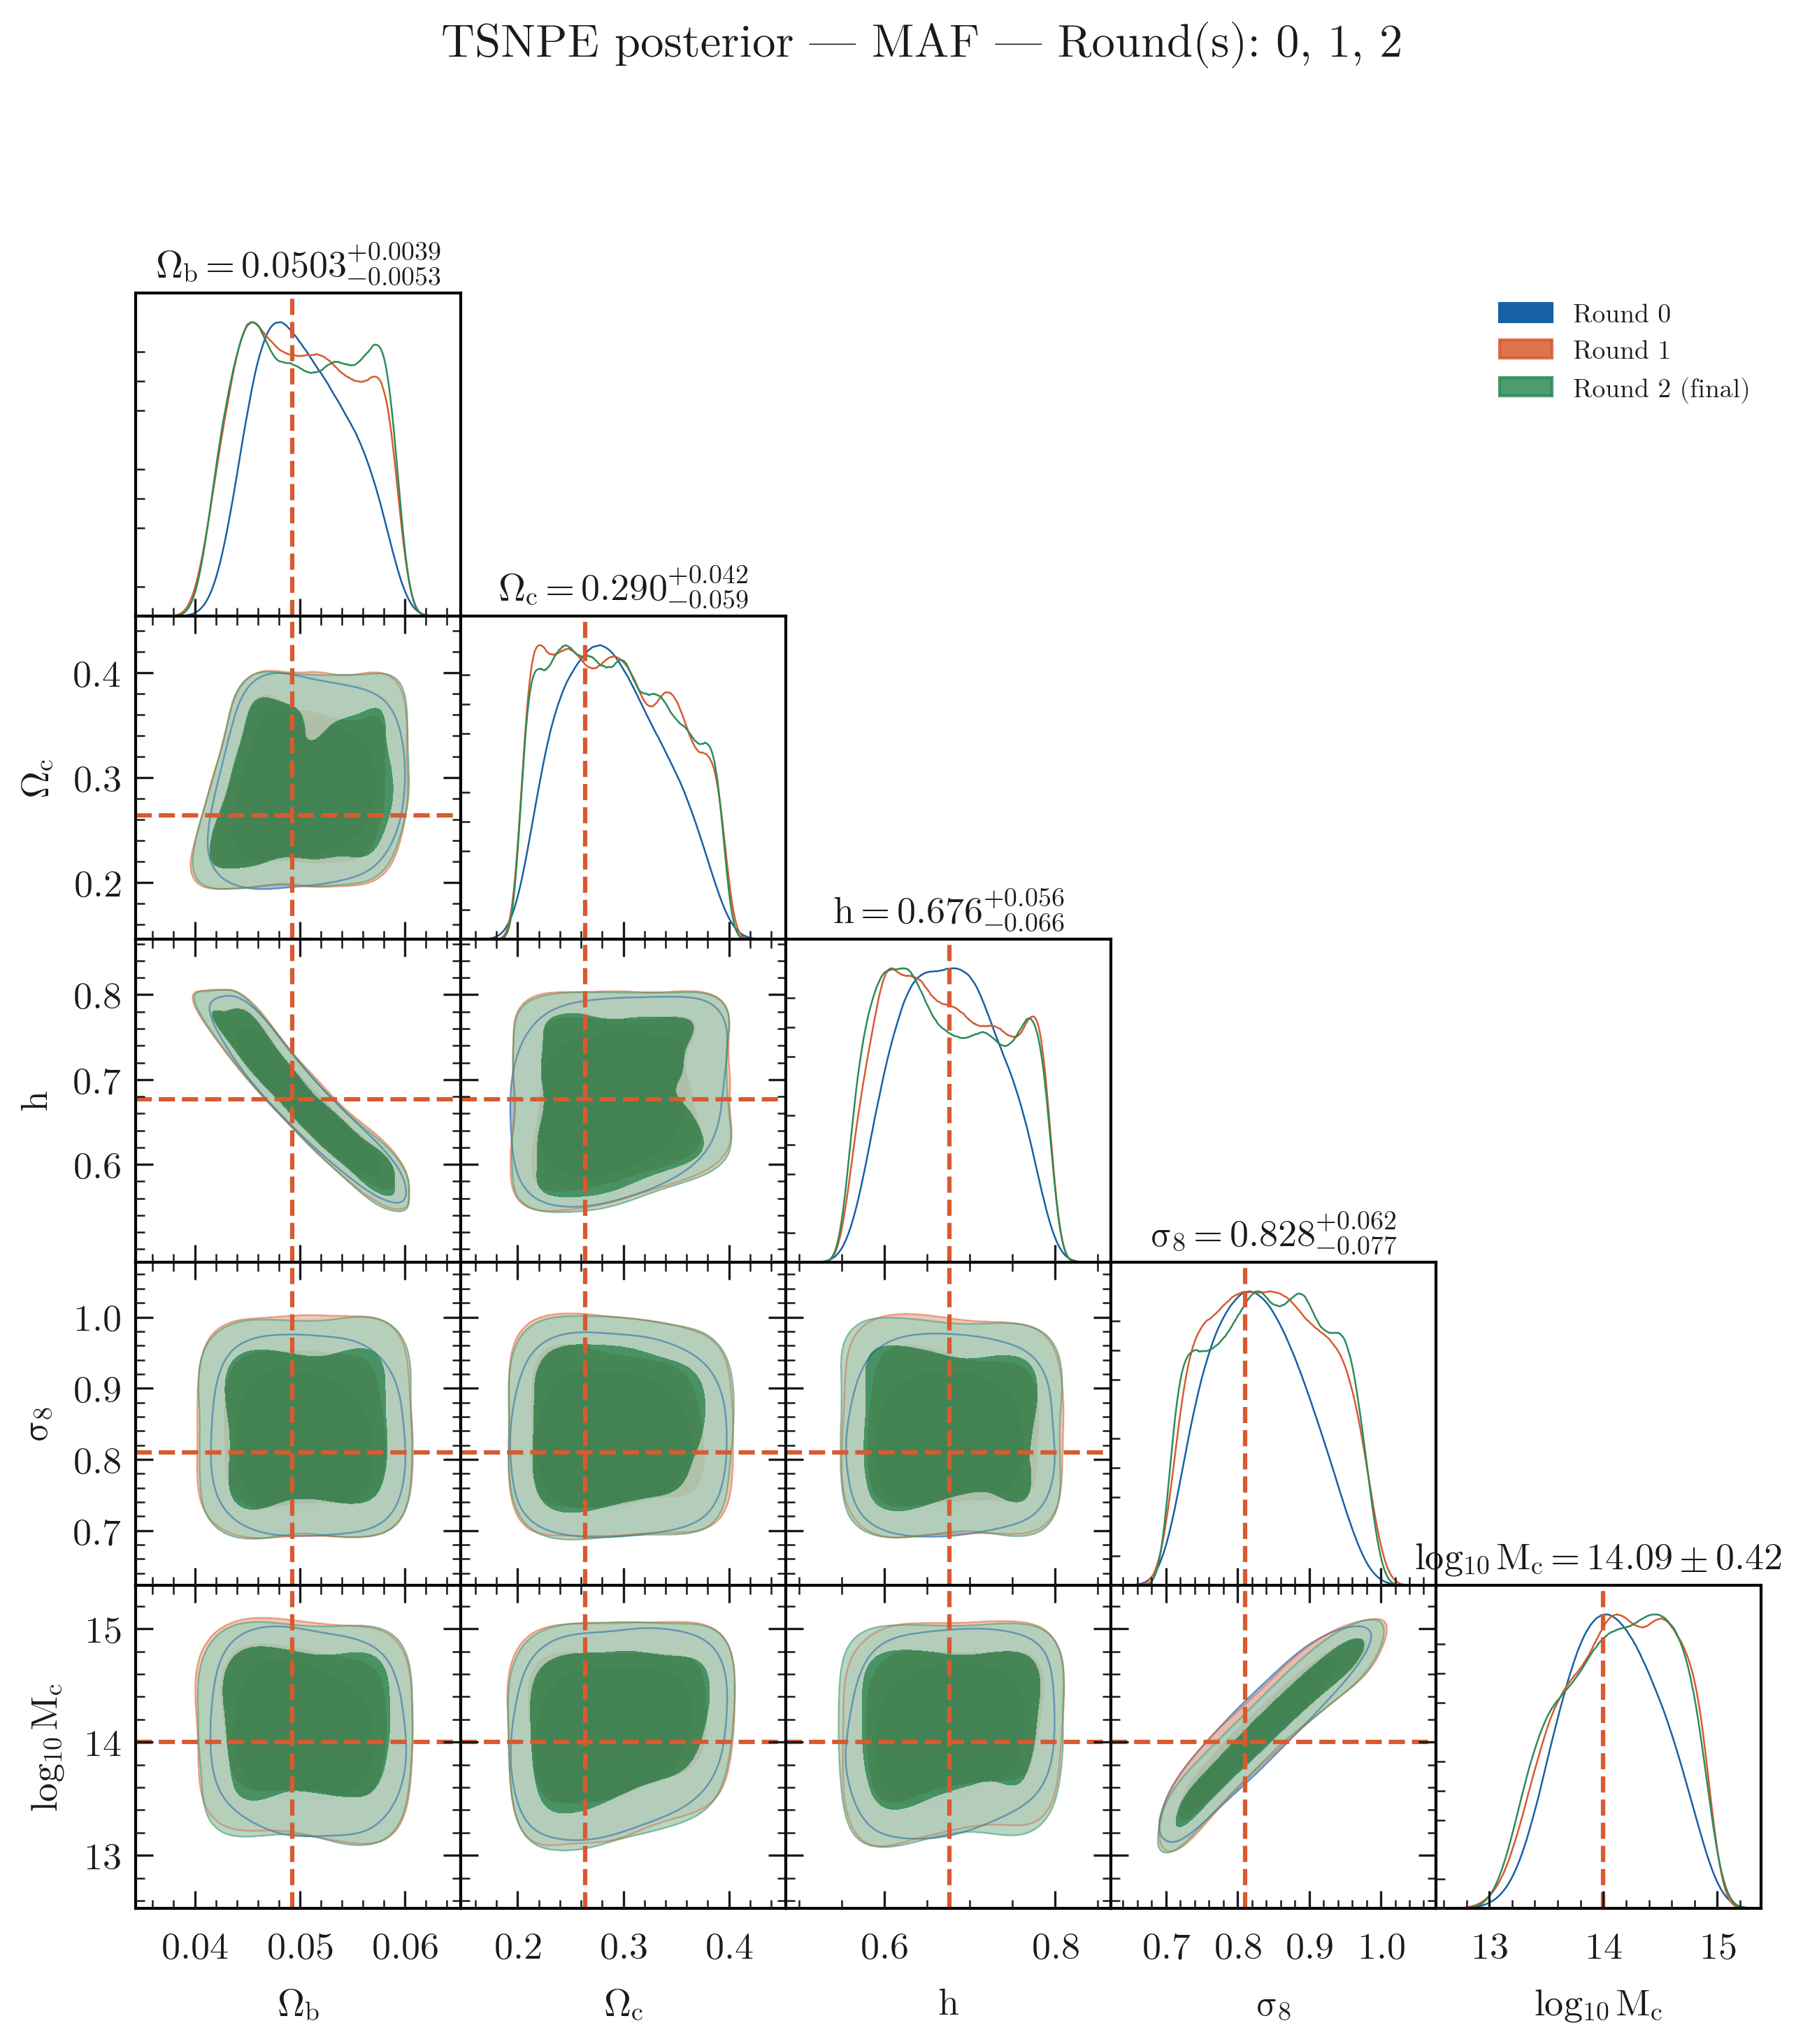
\includegraphics[width=0.9\textwidth]{figs/20260419_181315_fiducial_r00_r01_r02.png}
    \caption{Posterior distributions from SBI for the fiducial scenario.}
    \label{res_fig:sbi_fiducial}
\end{figure}

\begin{figure}[h!]
    \centering
    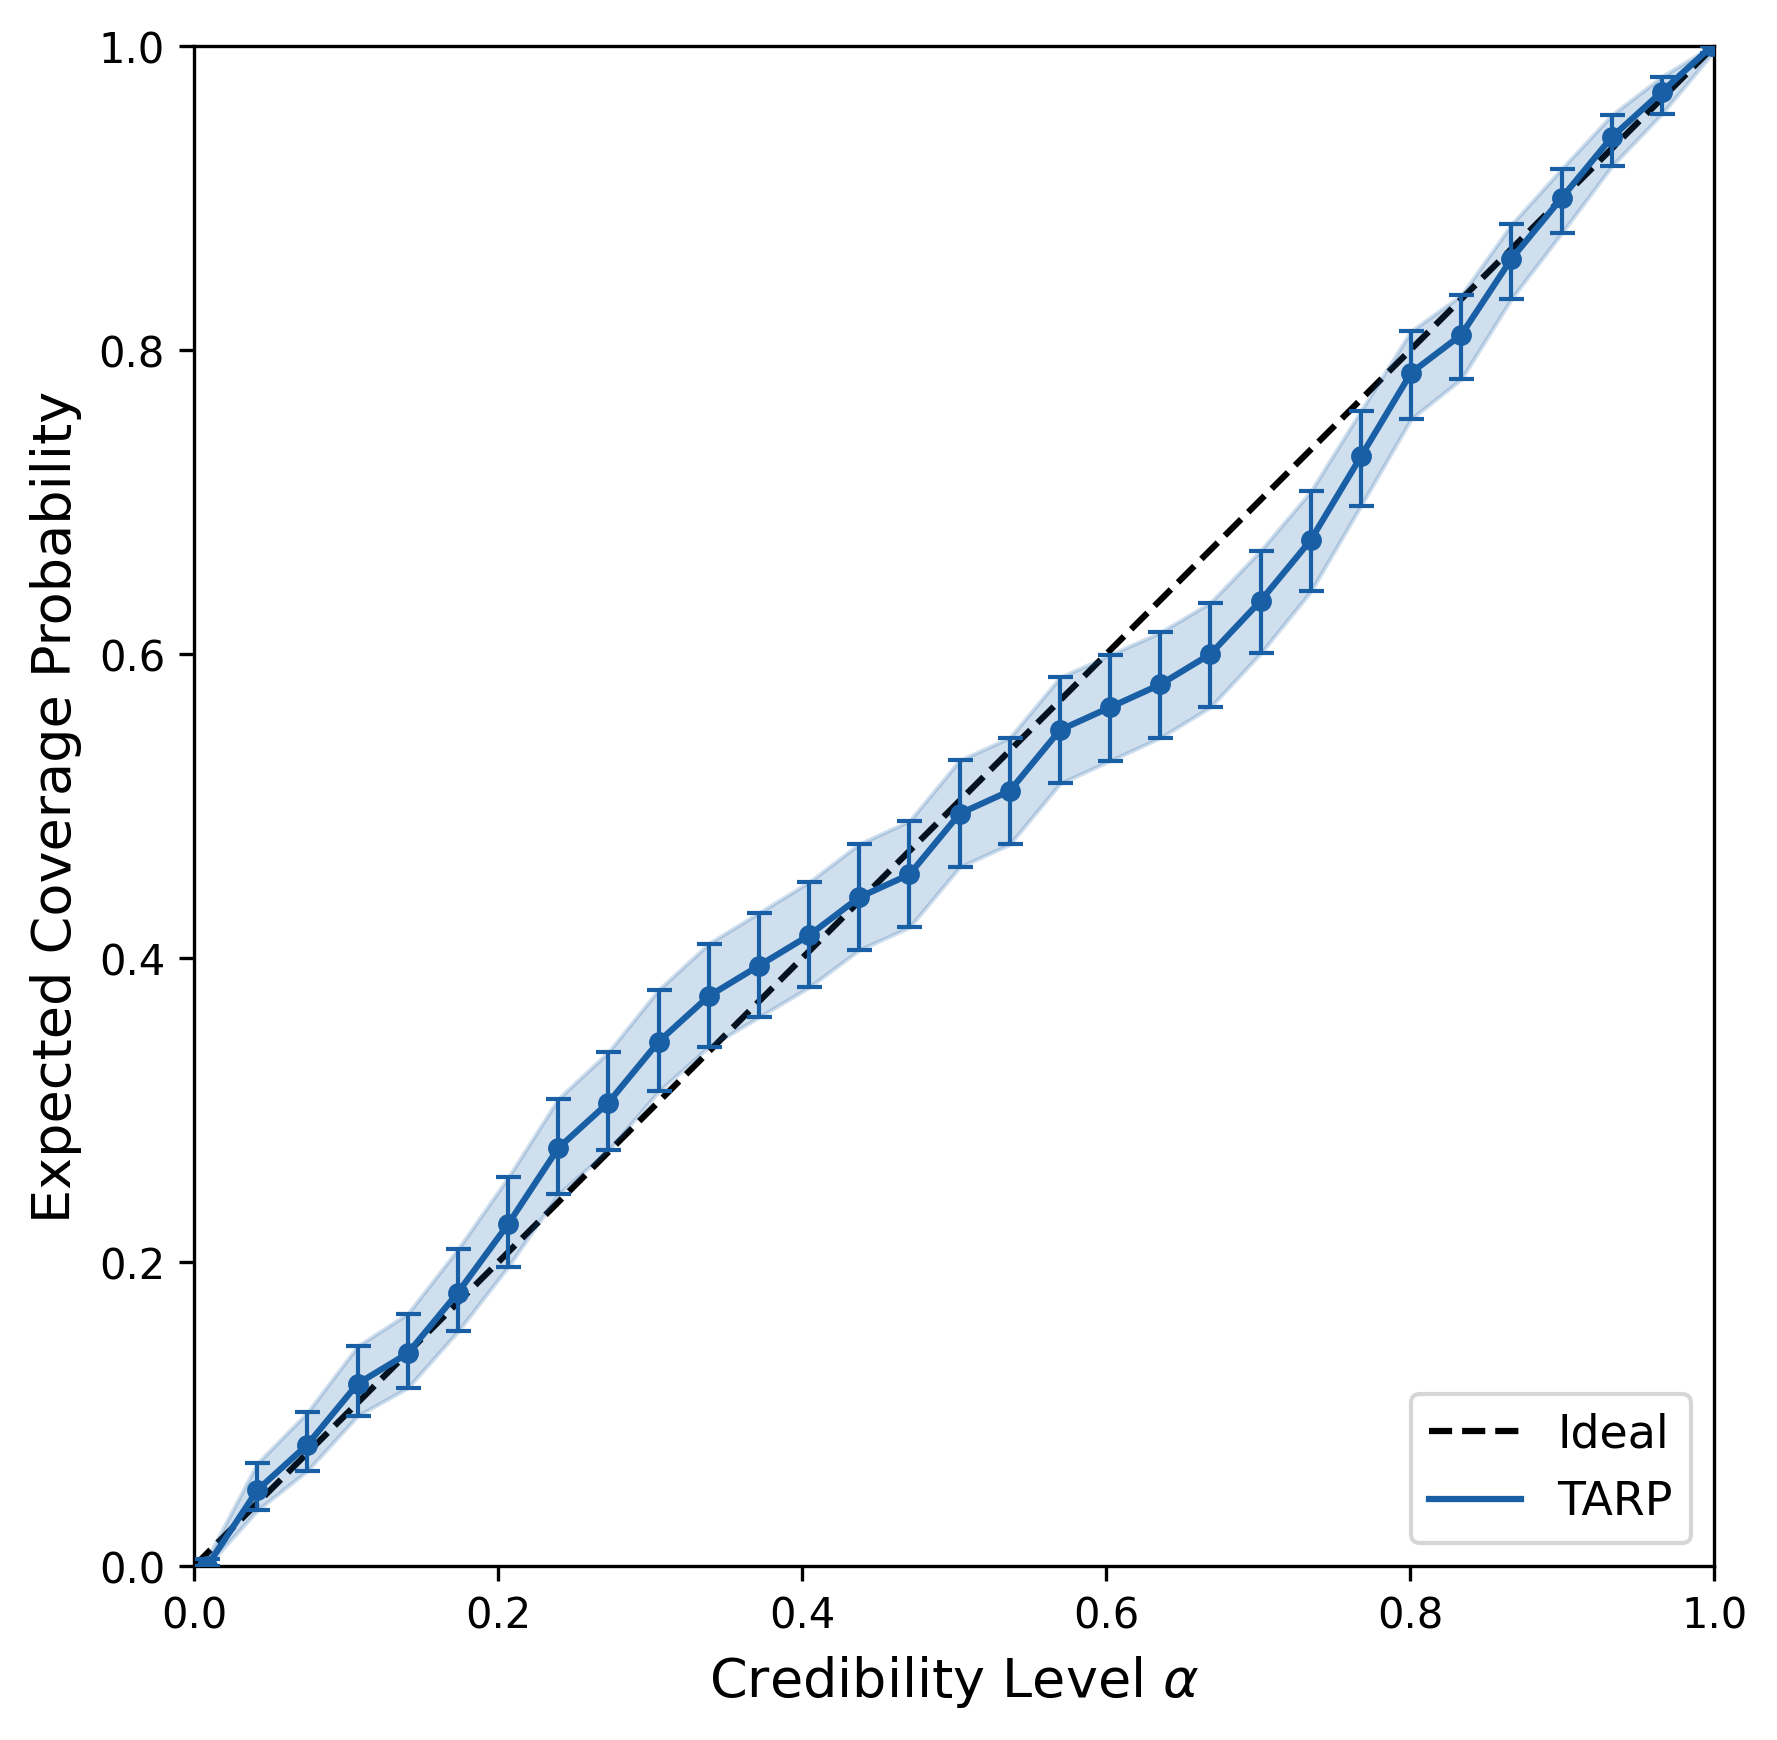
\includegraphics[width=0.5\textwidth]{figs/20260419_181315_fiducial_tarp.png}
    \caption{TARP coverage test for the fiducial SBI posterior.}
    \label{res_fig:sbi_tarp}
\end{figure}



In total, the score compression statistic is not sensitive to scale-dependent information. To perform inference with the simulation pipeline, the chosen summry statistic should include scale-depedent information such as the angular power spectrum. With the results given above, it is not possible to give a conclusive answer on the parameter bias that a systematic uncertinaty can have. The first step to do that is to choose an appropriate compression statistic which could ultimately have a different dimension as compared to the score compression, leading to a different optimal neural netwrok architecture to obtain a trustworthy posterior. Another choice of a summary statistic is the PDF, binned into a certain number of bins such that to reduce the nosie level of the PDF.